\documentclass[14pt,a4paper]{extarticle}

% ==============================================================================
% 1. CẤU HÌNH GÓI VÀ BẢNG MÃ TIẾNG VIỆT - 100% TIMES NEW ROMAN KHÔNG NGOẠI LỆ
% ==============================================================================
\usepackage{iftex}
\ifXeTeX
  \usepackage{fontspec}
  \setmainfont{Times New Roman}
  \setsansfont{Times New Roman}
  \setmonofont{Times New Roman}
  \renewcommand{\familydefault}{\rmdefault}
\else
  \usepackage[utf8]{inputenc}
  \usepackage[vietnamese]{babel}
  \usepackage[T5]{fontenc}
  \usepackage{mathptmx}
  \renewcommand{\rmdefault}{ptm}
  \renewcommand{\sfdefault}{ptm}
  \renewcommand{\ttdefault}{ptm}
  \renewcommand{\familydefault}{\rmdefault}
\fi
\usepackage{amsmath}
\usepackage{amssymb}

% Ép tất cả các lệnh điều chỉnh kích thước font về đúng 14pt (normalsize)
% Đảm bảo 100% toàn bộ tài liệu không có bất kỳ ngoại lệ nào về cỡ chữ
\let\tiny\normalsize
\let\scriptsize\normalsize
\let\footnotesize\normalsize
\let\small\normalsize
\let\large\normalsize
\let\Large\normalsize
\let\LARGE\normalsize
\let\huge\normalsize
\let\Huge\normalsize

% ==============================================================================
% 2. CĂN LỀ, GIÃN DÒNG 1.5 VÀ KHÔNG GIÃN CÁCH ĐOẠN (BEFORE=0PT, AFTER=0PT)
% ==============================================================================
% Căn lề chuẩn: Trái 3.0cm, Phải 2.0cm, Trên 2.0cm, Dưới 2.0cm
\usepackage[top=2cm, bottom=2cm, left=3cm, right=2cm, headheight=16pt, footskip=0.8cm]{geometry}
\raggedbottom

% Giãn cách dòng 1.5 cho toàn bộ văn bản (100% không có ngoại lệ)
\usepackage{setspace}
\setstretch{1.5}

% Thụt lề đầu dòng chuẩn 1.27cm (0.5 inch), tự động thụt lề cho cả đoạn đầu tiên
\usepackage{indentfirst}
\setlength{\parindent}{1.27cm}

% KHÔNG GIÃN CÁCH TRƯỚC / SAU ĐOẠN (Before = 0pt, After = 0pt, parskip = 0pt)
\setlength{\parskip}{0pt}
\emergencystretch=3em
\sloppy

% Bảng biểu nâng cao với giãn cách dòng 1.5 và căn giữa trục Y
\usepackage{booktabs}
\usepackage{tabularx}
\usepackage{longtable}
\usepackage{xltabular}
\usepackage{array}
\renewcommand{\tabularxcolumn}[1]{m{#1}}
\usepackage{float}
\usepackage{graphicx}
\graphicspath{{image/}{image/image_2/}{image/web/}}
\usepackage{tikz}
\usetikzlibrary{calc}
\usepackage{enumitem}
\usepackage[font=normalsize,labelfont=bf,labelsep=period,justification=centering,skip=4pt]{caption}
\captionsetup[figure]{name=Hình}
\captionsetup[table]{name=Bảng}
\renewcommand{\figurename}{Hình}
\renewcommand{\tablename}{Bảng}

% Điều chỉnh thu gọn khoảng cách quanh hình ảnh và caption
\setlength{\intextsep}{6pt plus 1pt minus 1pt}
\setlength{\textfloatsep}{6pt plus 1pt minus 1pt}
\setlength{\floatsep}{6pt plus 1pt minus 1pt}
\setlength{\abovecaptionskip}{4pt}
\setlength{\belowcaptionskip}{0pt}

% ==============================================================================
% 3. ĐỊNH DẠNG TIÊU ĐỀ (ĐỒNG NHẤT FONT TIMES NEW ROMAN, CỠ 14PT, GIÃN DÒNG 1.5)
% ==============================================================================
\usepackage{titlesec}
\usepackage{etoolbox}
\titleformat{\section}[block]
  {\normalfont\normalsize\bfseries\centering}
  {}{0pt}{}
\titlespacing*{\section}{0pt}{14pt}{6pt}

\titleformat{\subsection}[block]
  {\normalfont\normalsize\bfseries}
  {\thesubsection}{1em}{\normalsize\bfseries}
\titlespacing*{\subsection}{0pt}{10pt}{4pt}

\titleformat{\subsubsection}[block]
  {\normalfont\normalsize\bfseries}
  {\thesubsubsection}{1em}{\normalsize\bfseries}
\titlespacing*{\subsubsection}{0pt}{8pt}{3pt}

% Cho phép ngắt trang tự nhiên khi trang đầy mà không cắt lửng trang
\pretocmd{\subsection}{\par\pagebreak[3]}{}{}
\pretocmd{\subsubsection}{\par\pagebreak[3]}{}{}

% ==============================================================================
% 4. CẤU HÌNH MỤC LỤC VÀ DANH MỤC HÌNH ẢNH (TOC & LOF)
% ==============================================================================
\usepackage{tocloft}
\setcounter{tocdepth}{3}
\setcounter{secnumdepth}{3}

\renewcommand{\contentsname}{MỤC LỤC}
\renewcommand{\cfttoctitlefont}{\hfill\normalfont\normalsize\bfseries\MakeUppercase}
\renewcommand{\cftaftertoctitle}{\hfill}

% Cấu hình chấm dẫn đường và font chữ đồng nhất 14pt cho tất cả các cấp
\renewcommand{\cftsecleader}{\cftdotfill{\cftdotsep}}
\renewcommand{\cftsubsecleader}{\cftdotfill{\cftdotsep}}
\renewcommand{\cftsubsubsecleader}{\cftdotfill{\cftdotsep}}

\renewcommand{\cftsecfont}{\normalfont\normalsize\bfseries}
\renewcommand{\cftsubsecfont}{\normalfont\normalsize}
\renewcommand{\cftsubsubsecfont}{\normalfont\normalsize}

\renewcommand{\cftsecpagefont}{\normalfont\normalsize}
\renewcommand{\cftsubsecpagefont}{\normalfont\normalsize}
\renewcommand{\cftsubsubsecpagefont}{\normalfont\normalsize}

\setlength{\cftbeforesecskip}{4pt}
\setlength{\cftbeforesubsecskip}{1pt}
\setlength{\cftbeforesubsubsecskip}{0pt}

% Cấu hình Danh mục hình ảnh
\renewcommand{\listfigurename}{DANH MỤC HÌNH ẢNH}
\renewcommand{\cftloftitlefont}{\hfill\normalfont\normalsize\bfseries\MakeUppercase}
\renewcommand{\cftafterloftitle}{\hfill}
\renewcommand{\cftfigleader}{\cftdotfill{\cftdotsep}}
\renewcommand{\cftfigfont}{\normalfont\normalsize}
\renewcommand{\cftfigpagefont}{\normalfont\normalsize}
\renewcommand{\cftfigpresnum}{Hình }
\renewcommand{\cftfigaftersnum}{:}
\setlength{\cftfignumwidth}{2.2cm}
\setlength{\cftbeforefigskip}{4pt}

% Cấu hình Danh mục bảng biểu
\renewcommand{\listtablename}{DANH MỤC BẢNG BIỂU}
\renewcommand{\cftlottitlefont}{\hfill\normalfont\normalsize\bfseries\MakeUppercase}
\renewcommand{\cftafterlottitle}{\hfill}
\renewcommand{\cfttableader}{\cftdotfill{\cftdotsep}}
\renewcommand{\cfttabfont}{\normalfont\normalsize}
\renewcommand{\cfttabpagefont}{\normalfont\normalsize}
\renewcommand{\cfttabpresnum}{Bảng }
\renewcommand{\cfttabaftersnum}{:}
\setlength{\cfttabnumwidth}{2.2cm}
\setlength{\cftbeforetabskip}{4pt}

% ==============================================================================
% 5. CẤU HÌNH HEADER / FOOTER
% ==============================================================================
\usepackage{fancyhdr}
\pagestyle{fancy}
\fancyhf{}
\fancyfoot[R]{\normalfont\normalsize\thepage}
\renewcommand{\headrulewidth}{0pt}
\renewcommand{\footrulewidth}{0pt}

\fancypagestyle{plain}{%
    \fancyhf{}%
    \fancyfoot[R]{\normalfont\normalsize\thepage}%
    \renewcommand{\headrulewidth}{0pt}%
    \renewcommand{\footrulewidth}{0pt}%
}

% ==============================================================================
% 6. THÔNG TIN HYPERREF
% ==============================================================================
\usepackage{hyperref}
\hypersetup{
    colorlinks=true,
    hypertexnames=false,
    linkcolor=black,
    citecolor=black,
    urlcolor=blue,
    pdftitle={Báo cáo Đồ án DSA - Library Records-and-Decision Engine},
    pdfauthor={Nhóm 06}
}
\usepackage{bookmark}
\bookmarksetup{
    open=true,
    depth=3,
    numbered=false
}

% ==============================================================================
% BẮT ĐẦU TÀI LIỆU
% ==============================================================================
\begin{document}
\pagenumbering{gobble}
\pagestyle{empty}
\thispagestyle{empty}

% ==============================================================================
% 1. TRANG BÌA
% ==============================================================================
\begin{titlepage}
    \begin{tikzpicture}[remember picture, overlay]
        \draw[line width=1.5pt]
            ($(current page.north west) + (2.0cm,-1.8cm)$)
            rectangle
            ($(current page.south east) + (-1.5cm,1.8cm)$);
        \draw[line width=0.5pt]
            ($(current page.north west) + (2.12cm,-1.92cm)$)
            rectangle
            ($(current page.south east) + (-1.62cm,1.92cm)$);
    \end{tikzpicture}
    \centering
    \fontsize{14pt}{17pt}\selectfont
    \textbf{TRƯỜNG ĐẠI HỌC CÔNG NGHỆ KỸ THUẬT TP. HỒ CHÍ MINH}\\
    \textbf{KHOA CÔNG NGHỆ THÔNG TIN}\\
    \textbf{BỘ MÔN CÔNG NGHỆ PHẦN MỀM}\\[0.35cm]

    
\includegraphics[width=4.8cm]{LOGO.png}\\[0.35cm]

    \textbf{TIỂU LUẬN HỌC PHẦN CẤU TRÚC DỮ LIỆU VÀ GIẢI THUẬT}\\[0.45cm]

    \fontsize{14pt}{18pt}\selectfont
    \textbf{HỆ THỐNG QUẢN LÝ TÀI LIỆU THƯ VIỆN VÀ ENGINE ĐỐI SÁNH}\\
    \textbf{HIỆU NĂNG THUẬT TOÁN (DSA)}\\[0.25cm]
    \textbf{LIBRARY RECORDS-AND-DECISION ENGINE}\\[0.75cm]

    \fontsize{14pt}{17pt}\selectfont
    \begin{flushleft}
        \hspace{1.2cm}\textbf{Giảng viên hướng dẫn:} ThS. Bảo Vũ Đình (T-Bao)\\[0.15cm]
        \hspace{1.2cm}\textbf{Mã lớp học phần:} 261DASA230179\_06\\[0.15cm]
        \hspace{1.2cm}\textbf{Nhóm thực hiện:} Nhóm 06\\[0.15cm]
        \hspace{1.2cm}\textbf{Sinh viên thực hiện:}\\[0.1cm]
        \hspace{1.5cm}\begin{tabular}{ll}
            \textbf{Họ và tên} & \textbf{MSSV} \\
            Trần Quốc Việt Nam (Nhóm trưởng) & 25110274 \\
            Lê Thị Tuyết Nhi & 25110283 \\
            Lê Nhật Ninh & 25110288 \\
            Nguyễn Ngọc Hồng Nhung & 25110285 \\
            Trần Phạm Huỳnh Như & 25110286 \\
        \end{tabular}
    \end{flushleft}

    \vfill
    \fontsize{14pt}{17pt}\selectfont
    \textit{TP. Hồ Chí Minh, tháng 10 năm 2026}
\end{titlepage}

% ------------------------------------------------------------------------------
% TRANG: LỜI CẢM ƠN
% ------------------------------------------------------------------------------
\newpage
\thispagestyle{empty}
\section*{LỜI CẢM ƠN}

Lời đầu tiên, Nhóm 06 chúng em xin chân thành gửi lời cảm ơn sâu sắc nhất đến Ban Giám hiệu Trường Đại học Công nghệ Kỹ thuật TP. Hồ Chí Minh cùng toàn thể quý Thầy Cô Khoa Công nghệ Thông tin đã tạo mọi điều kiện học tập thuận lợi và trang bị cho chúng em nền tảng tư duy khoa học máy tính vững chắc.

Đặc biệt, chúng em xin bày tỏ lòng tri ân sâu sắc đến Thầy ThS. Bảo Vũ Đình (T-Bao) --- giảng viên phụ trách học phần Cấu trúc Dữ liệu và Giải thuật (Mã lớp học phần: 261DASA230179\_06). Trong suốt học kỳ vừa qua, Thầy đã luôn mang đến cho chúng em những bài giảng giàu tính học thuật, rèn luyện tư duy phản biện thuật toán và phương pháp tiếp cận vấn đề theo chuẩn kỹ sư chuyên nghiệp. Sự định hướng tận tâm của Thầy đã giúp chúng em thấu hiểu sâu sắc bản chất tối ưu hóa trên bộ nhớ chính (In-Memory Engine) và hoàn thành tốt đồ án capstone này.

Chúng em xin trân trọng tiếp thu mọi ý kiến đóng góp quý báu từ Thầy để hoàn thiện hơn nữa kiến thức và kỹ năng lập trình giải thuật trên con đường học tập phía trước. Kính chúc Thầy luôn dồi dào sức khỏe, hạnh phúc và luôn gặt hái được nhiều thành công trong sự nghiệp giảng dạy!

\vspace{1.0cm}
\begin{flushright}
    TP. Hồ Chí Minh, ngày 03 tháng 10 năm 2026\\[0.2cm]
    \textbf{Sinh viên thực hiện}\\[0.2cm]
    \textbf{Nhóm 06}
\end{flushright}

% ------------------------------------------------------------------------------
% TRANG: BẢNG ĐÁNH GIÁ VÀ PHÂN CÔNG NHIỆM VỤ
% ------------------------------------------------------------------------------
\newpage
\thispagestyle{empty}
\begingroup
\titlespacing*{\section}{0pt}{0pt}{4pt}
\section*{BẢNG ĐÁNH GIÁ VÀ PHÂN CÔNG NHIỆM VỤ}

\vspace{-0.25cm}
\noindent
\textbf{Mã lớp học phần:} 261DASA230179\_06\\[0.1cm]
\textbf{Nhóm thực hiện:} Nhóm 06\\[0.1cm]
\textbf{Giảng viên hướng dẫn:} ThS. Bảo Vũ Đình (T-Bao)\\[0.25cm]
\noindent
\begingroup
\setstretch{0.92}
\setlength{\tabcolsep}{3pt}
\renewcommand{\arraystretch}{1.0}
\begin{tabularx}{\linewidth}{|>{\centering\arraybackslash}m{1.2cm}|>{\raggedright\arraybackslash}m{3.5cm}|>{\raggedright\arraybackslash}X|>{\centering\arraybackslash}m{2.2cm}|}
\hline
\textbf{STT} & \textbf{Họ và tên / MSSV} & \textbf{Nhiệm vụ phân công} & \textbf{Hoàn thành} \\ \hline
1 & \textbf{Nguyễn Ngọc Hồng Nhung}\newline MSSV: 25110285 & Phụ trách tầng Lưu trữ bền vững (Persistence Layer: Nạp và lưu trữ dữ liệu an toàn từ các tệp JSON vào In-Memory Engine). & 100\% \\ \hline
2 & \textbf{Trần Quốc Việt Nam}\newline (Trưởng nhóm)\newline MSSV: 25110274 & Điều phối chung dự án và phụ trách toàn bộ hệ thống Bảng băm gồm: MC1 (Tra cứu Mã Sách), RQ1 (Phân cụm Thể loại), và RQ3 (Chỉ mục ngược Inverted Index). & 100\% \\ \hline
3 & \textbf{Lê Nhật Ninh}\newline MSSV: 25110288 & Phụ trách Cây đống cực đại Max-Heap (MC2: Top sách mượn nhiều nhất) và Cây tự cân bằng AVL (RQ2: Truy vết phiếu quá hạn). & 100\% \\ \hline
4 & \textbf{Lê Thị Tuyết Nhi}\newline MSSV: 25110283 & Phụ trách tầng Trình diễn (Giao diện dòng lệnh TUI) và định nghĩa các Cấu trúc dữ liệu cơ bản (struct Book, Reader, BorrowRecord) cùng khung sườn các hàm. & 100\% \\ \hline
5 & \textbf{Trần Phạm Huỳnh Như}\newline MSSV: 25110286 & Phụ trách đọc hiểu toàn bộ hệ thống, xây dựng kịch bản và thực hiện quay video thuyết trình demo sản phẩm thời lượng 5 phút. & 100\% \\ \hline
\end{tabularx}
\endgroup

\vspace{0.25cm}
\noindent
Đánh giá kết quả: Toàn bộ 5 thành viên hoàn thành 100\% nhiệm vụ đúng tiến độ, nắm vững nguyên lý cấu trúc dữ liệu tự cài đặt và phối hợp tích hợp hệ sinh thái đồng bộ.
\endgroup

% ------------------------------------------------------------------------------
% TRANG: TUYÊN BỐ QUYỀN SỞ HỮU THÀNH PHẦN - D3
% ------------------------------------------------------------------------------
\newpage
\thispagestyle{empty}
\begingroup
\titlespacing*{\section}{0pt}{0pt}{4pt}
\section*{TUYÊN BỐ QUYỀN SỞ HỮU THÀNH PHẦN - D3}

\vspace{-0.25cm}
\noindent
Tuân thủ quy định đánh giá năng lực cá nhân theo đề bài học phần DASA230179, từng thành viên xác nhận quyền sở hữu kỹ thuật, trách nhiệm cài đặt và lập luận thiết kế độc lập như sau:

\vspace{0.15cm}
\noindent
\begingroup
\setstretch{0.90}
\setlength{\tabcolsep}{3pt}
\renewcommand{\arraystretch}{0.95}
\begin{tabularx}{\linewidth}{|>{\raggedright\arraybackslash}m{3.1cm}|>{\raggedright\arraybackslash}m{2.8cm}|>{\raggedright\arraybackslash}X|}
\hline
\textbf{Thành viên \& MSSV} & \textbf{Thành phần sở hữu} & \textbf{Đóng góp Kỹ thuật \& Biện minh Thiết kế} \\ \hline
\textbf{Nguyễn Ngọc Hồng Nhung}\newline MSSV: 25110285 & \textbf{Persistence Layer} & Thiết kế cơ chế đồng bộ đĩa-RAM tại lớp FileStore (nạp và lưu trữ tệp JSON, xử lý ngoại lệ và kiểm soát tính toàn vẹn dữ liệu). \\ \hline
\textbf{Trần Quốc Việt Nam}\newline (Trưởng nhóm)\newline MSSV: 25110274 & \textbf{Hệ thống Bảng băm}\newline \textit{(MC1, RQ1, RQ3)} & Tự cài đặt Bảng băm Separate Chaining (DJB2) cho MC1, CategoryHashTable cho RQ1 và InvertedIndex cho RQ3; điều phối chung. \\ \hline
\textbf{Lê Nhật Ninh}\newline MSSV: 25110288 & \textbf{Max-Heap \& Cây AVL}\newline \textit{(MC2, RQ2)} & Cài đặt Cây đống cực đại Max-Heap Floyd cho MC2 (Top sách) và Cây tự cân bằng AVL 4 phép quay cho RQ2 (Truy vết quá hạn). \\ \hline
\textbf{Lê Thị Tuyết Nhi}\newline MSSV: 25110283 & \textbf{Presentation TUI \& Data Models} & Thiết kế giao diện dòng lệnh TUI tương tác, định nghĩa mô hình dữ liệu lõi (struct Book, Reader, BorrowRecord) và khung hàm. \\ \hline
\textbf{Trần Phạm Huỳnh Như}\newline MSSV: 25110286 & \textbf{Kịch bản \& Video Thuyết trình 5p} & Nghiên cứu toàn diện luồng nghiệp vụ, xây dựng kịch bản thuyết trình và trực tiếp quay dựng video demo 5 phút minh họa đồ án. \\ \hline
\end{tabularx}
\endgroup

\vspace{0.25cm}
\noindent
Cam kết cá nhân: Toàn thể 5 thành viên cam kết nắm vững toàn bộ mã nguồn do mình chịu trách nhiệm, thấu hiểu tường tận chứng minh độ phức tạp toán học và sẵn sàng giải trình độc lập trong buổi vấn đáp bảo vệ đồ án.
\endgroup

% ------------------------------------------------------------------------------
% MỤC LỤC & DANH MỤC HÌNH ẢNH & DANH MỤC BẢNG BIỂU
% ------------------------------------------------------------------------------
\newpage
\thispagestyle{empty}
\tableofcontents

\newpage
\thispagestyle{empty}
\listoffigures

\newpage
\thispagestyle{empty}
\listoftables

% ------------------------------------------------------------------------------
% DANH MỤC TỪ VIẾT TẮT
% ------------------------------------------------------------------------------
\newpage
\thispagestyle{empty}
\section*{DANH MỤC TỪ VIẾT TẮT}

\begin{table}[H]
\centering
\begingroup
\setstretch{1.15}
\setlength{\tabcolsep}{4pt}
\renewcommand{\arraystretch}{1.15}
\begin{tabularx}{\linewidth}{|>{\bfseries\centering\arraybackslash}m{2.3cm}|>{\raggedright\arraybackslash}m{5.5cm}|>{\raggedright\arraybackslash}X|}
\hline
\textbf{Ký hiệu} & \textbf{Thuật ngữ tiếng Anh} & \textbf{Ý nghĩa tiếng Việt} \\ \hline
DSA & Data Structures and Algorithms & Cấu trúc Dữ liệu và Giải thuật \\ \hline
MC & Mandatory Criteria & Yêu cầu nghiệp vụ bắt buộc chung \\ \hline
MC1 & Mandatory Criteria 1 & Tra cứu chính xác sách theo Mã định danh \\ \hline
MC2 & Mandatory Criteria 2 & Truy xuất Top sách được mượn nhiều nhất \\ \hline
RQ & Required Query & Yêu cầu truy vấn tự phát hiện đặc thù \\ \hline
RQ1 & Required Query 1 & Phân loại và lọc sách theo Thể loại \\ \hline
RQ2 & Required Query 2 & Truy vết phiếu mượn quá hạn theo khoảng ngày \\ \hline
RQ3 & Required Query 3 & Tìm kiếm tựa sách qua Chỉ mục ngược \\ \hline
AVL & Adelson-Velsky and Landis Tree & Cây nhị phân tìm kiếm tự cân bằng AVL \\ \hline
JDN & Julian Day Number & Số ngày Julius (chuẩn hóa mốc thời gian $O(1)$) \\ \hline
TUI & Terminal User Interface & Giao diện người dùng trên dòng lệnh Terminal \\ \hline
RAM & Random Access Memory & Bộ nhớ truy xuất ngẫu nhiên khả biến \\ \hline
JSON & JavaScript Object Notation & Định dạng hoán chuyển dữ liệu văn bản chuẩn \\ \hline
CLO & Course Learning Outcomes & Chuẩn đầu ra tích hợp của học phần \\ \hline
\end{tabularx}
\endgroup
\end{table}

% ==============================================================================
% PHẦN MỞ ĐẦU
% ==============================================================================
\newpage
\pagestyle{fancy}
\pagenumbering{arabic}
\setcounter{page}{1}
\section*{PHẦN MỞ ĐẦU}
\addcontentsline{toc}{section}{PHẦN MỞ ĐẦU}

\subsection*{1. Lý do chọn đề tài và bối cảnh thực tiễn của bài toán}
\addcontentsline{toc}{subsection}{1. Lý do chọn đề tài và bối cảnh thực tiễn của bài toán}

Trong các trung tâm thông tin thư viện đại học và các nền tảng học liệu số hiện đại, khối lượng đầu sách và nhật ký mượn/trả tài liệu không ngừng gia tăng theo cấp số nhân qua các năm học. Hệ thống quản lý thư viện không chỉ đơn thuần là nơi lưu trữ thông tin tĩnh, mà đóng vai trò là một động cơ xử lý hồ sơ và hỗ trợ ra quyết định (\textit{Records-and-Decision Engine})\footnote{Records-and-Decision Engine: Hệ thống phần mềm hợp nhất lưu trữ tập hợp bản ghi lớn và trả lời tức thì các câu hỏi vận hành cốt lõi ngay cả khi dữ liệu liên tục thay đổi.} thời gian thực. Động cơ này phải phản hồi tức thì các yêu cầu nghiệp vụ cấp thiết: tra cứu tức thì tình trạng một đầu sách phục vụ độc giả tại quầy, thống kê Top sách mượn nhiều nhất để tái cung ứng tài liệu, phân cụm sách theo thể loại nghiên cứu, kiểm soát danh sách mượn quá hạn để gửi thông báo phạt trễ và tìm kiếm nhanh tựa sách theo từ khóa linh hoạt.

Khi dữ liệu thư viện mở rộng quy mô lớn, các giải pháp tìm kiếm vét cạn tuyến tính ($O(N)$) hay quét xâu con $O(N \times M)$ bộc lộ điểm nghẽn nghiêm trọng, làm chậm hệ thống và lãng phí tài nguyên CPU. Việc áp dụng các cấu trúc dữ liệu chuyên biệt trong bộ nhớ chính (In-Memory Data Structures) như Bảng băm xích rời (Separate Chaining Hash Table), Cây đống cực đại (Max-Heap), Cây tự cân bằng AVL (AVL Tree) và Bảng băm chỉ mục ngược (Inverted Index) là giải pháp tiên quyết để tối ưu hóa thời gian phản hồi về mức $O(1)$, $O(\log N)$, $O(1+K)$ và $O(\log N + K)$. Xuất phát từ nhu cầu thực tiễn đó, Nhóm 06 triển khai đề tài: ''Hệ thống Quản lý Tài liệu Thư viện và Engine Đối sánh Hiệu năng Thuật toán (DSA) -- Library Records-and-Decision Engine''.

\subsection*{2. Mục tiêu nghiên cứu và chuẩn đầu ra học phần (CLO Alignment)}
\addcontentsline{toc}{subsection}{2. Mục tiêu nghiên cứu và chuẩn đầu ra học phần (CLO Alignment)}

Đồ án được thiết kế bám sát và hiện thực hóa các chuẩn đầu ra cốt lõi của học phần Cấu trúc Dữ liệu và Giải thuật (DASA230179).

Thứ nhất, đối với chuẩn CLO1 về mô hình hóa và lập luận tính đúng đắn, nhóm tiến hành phân tích toàn diện không gian bài toán, xác định tập thuộc tính thực thể, thiết lập các ràng buộc dữ liệu chặt chẽ và xử lý triệt để các trường hợp biên đặc biệt như dữ liệu rỗng, mảng đơn phần tử hay khóa tìm kiếm không tồn tại.

Thứ hai, đối với chuẩn CLO3 về cài đặt cấu trúc dữ liệu cốt lõi from-scratch, toàn bộ 5 cấu trúc nòng cốt gồm Bảng băm xích rời với hàm băm DJB2, Cây đống cực đại Max-Heap với thuật toán Floyd, Cây tự cân bằng AVL 4 phép quay và Bảng băm chỉ mục ngược Inverted Index đều được các thành viên tự tay cài đặt hoàn toàn trên chuẩn ngôn ngữ C++17, tuyệt đối không phụ thuộc vào các cấu trúc dựng sẵn trong thư viện STL như \texttt{std::map}, \texttt{std::priority\_queue} hay \texttt{std::unordered\_map}\footnote{Tuân thủ yêu cầu nghiêm ngặt theo Mục 6.2 của đề bài: Toàn bộ các cấu trúc nòng cốt phải tự cài đặt from-scratch để minh chứng năng lực lập trình và tư duy thuật toán cá nhân.}.

Thứ ba, đối với chuẩn CLO7 về cấu trúc phân cấp và kiểm soát suy thoái, đồ án khảo sát chi tiết cấu trúc phân cấp cây đống và cây AVL, phân tích hệ số cân bằng (Balance Factor), cơ chế quay cây $O(1)$ và các kịch bản suy thoái độ phức tạp nhằm đảm bảo hệ thống luôn duy trì trần giới hạn thời gian thực thi trong trường hợp xấu nhất.

Thứ tư, đối với chuẩn CLO8 về capstone và bảo vệ cấu trúc dữ liệu, nhóm phân tích sâu sắc các mô thức truy cập dữ liệu (Access Patterns), áp dụng ma trận 7 tiêu chí kỹ thuật và quy trình 4 câu hỏi quyết định Q1--Q4 để biện minh thuyết phục cho từng lựa chọn cấu trúc trong hệ thống.

\subsection*{3. Đối tượng, phạm vi nghiên cứu và tập dữ liệu thử nghiệm}
\addcontentsline{toc}{subsection}{3. Đối tượng, phạm vi nghiên cứu và tập dữ liệu thử nghiệm}

Về đối tượng nghiên cứu, đề tài tập trung vào các cấu trúc dữ liệu trên bộ nhớ chính (RAM-based) và các thuật toán nâng cao phục vụ 5 bài toán nghiệp vụ: Tra cứu mã sách (MC1), Top sách mượn nhiều nhất (MC2), Lọc theo thể loại (RQ1), Truy vết mượn quá hạn (RQ2) và Tìm kiếm từ khóa tựa sách (RQ3). Về tập dữ liệu thử nghiệm, hệ thống nạp các tệp dữ liệu chuẩn \texttt{data/books.json}, \texttt{data/borrow\_records.json} và \texttt{data/readers.json}.

\subsection*{4. Phương pháp tiếp cận, công cụ thực hiện và bố cục báo cáo}
\addcontentsline{toc}{subsection}{4. Phương pháp tiếp cận, công cụ thực hiện và bố cục báo cáo}

Phương pháp tiếp cận kết hợp chặt chẽ giữa phân tích toán học lý thuyết ($O, \Omega, \Theta$) với thực nghiệm đo đạc Benchmark tự động bằng đồng hồ xung nhịp microsecond (\texttt{std::chrono::high\_resolution\_clock})\footnote{Thư viện đo thời gian chính xác cao theo đặc tả chuẩn ISO/IEC C++20.} qua $K=1000$ đến $K=5000$ lần lặp kèm giai đoạn warm-up CPU.

Về bố cục báo cáo, tài liệu được tổ chức thành đúng 2 chương trọng tâm. Chương 1 tập trung vào tổng quan bài toán và thiết kế cấu trúc dữ liệu, trình bày bối cảnh, mô hình hóa dữ liệu, phân tích xung đột yêu cầu và áp dụng ma trận 7 tiêu chí Q1--Q4 để biện minh cấu trúc. Chương 2 đi sâu vào thiết kế kiến trúc 3 tầng, hiện thực mã nguồn C++ from-scratch cho 5 cặp thuật toán đối chứng, sơ đồ tuần tự Sequence Diagram, chứng minh định lý toán học, kết quả Benchmark đa kịch bản và phản ánh đóng góp cá nhân.

% ==============================================================================
% CHƯƠNG 1: TỔNG QUAN BÀI TOÁN VÀ THIẾT KẾ CẤU TRÚC DỮ LIỆU
% ==============================================================================
\newpage
\section*{CHƯƠNG 1: TỔNG QUAN BÀI TOÁN\\VÀ THIẾT KẾ CẤU TRÚC DỮ LIỆU}
\addcontentsline{toc}{section}{CHƯƠNG 1: TỔNG QUAN BÀI TOÁN VÀ THIẾT KẾ CẤU TRÚC DỮ LIỆU}

\subsection*{1.1. Mô tả bài toán và phân tích nghiệp vụ hệ thống}
\addcontentsline{toc}{subsection}{1.1. Mô tả bài toán và phân tích nghiệp vụ hệ thống}

\subsubsection*{1.1.1. Bối cảnh bài toán Library Records-and-Decision Engine}
\addcontentsline{toc}{subsubsection}{1.1.1. Bối cảnh bài toán Library Records-and-Decision Engine}

Trong bối cảnh chuyển đổi số giáo dục đại học và tự động hóa các trung tâm học liệu, thư viện hiện đại không chỉ đóng vai trò là một kho chứa sách vật lý truyền thống mà đã trở thành một trung tâm điều phối tri thức tích hợp. Một hệ thống thư viện phục vụ hàng chục nghìn độc giả với hàng trăm nghìn đầu tài liệu học thuật đòi hỏi năng lực phản hồi tức thì đối với mọi thao tác vận hành hàng ngày. Hệ thống phần mềm đóng vai trò là một động cơ quản lý hồ sơ và hỗ trợ ra quyết định, chịu trách nhiệm lưu trữ toàn bộ các thực thể bản ghi ngày càng gia tăng theo thời gian, đồng thời phải đưa ra câu trả lời chính xác, tức thì cho các câu hỏi nghiệp vụ ngay cả khi dữ liệu liên tục biến động do các hoạt động mượn và trả sách diễn ra liên tục.

Người sử dụng hệ thống bao gồm hai nhóm đối tượng chính với các kỳ vọng hoàn toàn khác nhau. Độc giả cần tra cứu nhanh chóng sự hiện diện của một đầu sách, tìm kiếm tài liệu theo chủ đề nghiên cứu hoặc tìm kiếm theo các từ khóa có trong tựa sách để phục vụ học tập. Trong khi đó, nhân viên quản lý thư viện cần nắm bắt chính xác mức độ quan tâm của độc giả đối với từng đầu sách nhằm lên kế hoạch bổ sung nguồn tài liệu, đồng thời phải thường xuyên rà soát các phiếu mượn đã vượt quá thời hạn quy định để gửi thông báo nhắc nhở và xử lý phạt trễ. Cả hai nhóm người dùng đều không quan tâm đến việc hệ thống bên dưới sử dụng cấu trúc dữ liệu cụ thể nào; họ chỉ yêu cầu phần mềm phản hồi tức thời, không xuất hiện độ trễ cảm nhận được và duy trì tính toàn vẹn dữ liệu trong suốt quá trình vận hành.

\subsubsection*{1.1.2. Mô hình hóa thực thể dữ liệu và các trường thuộc tính}
\addcontentsline{toc}{subsubsection}{1.1.2. Mô hình hóa thực thể dữ liệu và các trường thuộc tính}

Để hệ thống có thể quản trị toàn diện các nghiệp vụ thư viện, các đối tượng trong thế giới thực được trừu tượng hóa và mô hình hóa thành các cấu trúc bản ghi cụ thể trong bộ nhớ chính. Hệ thống tập trung quản lý ba thực thể dữ liệu nòng cốt, bao gồm Tài liệu, Độc giả và Phiếu mượn trả.

Thực thể Tài liệu đại diện cho từng đầu sách được lưu trữ trong thư viện, bao gồm các trường thuộc tính định danh mã sách duy nhất dưới dạng chuỗi ký tự, tên tài liệu, tên tác giả, thể loại chuyên ngành, năm xuất bản, số lượng sách tồn kho hiện có tại thư viện và bộ đếm tổng số lượt mượn tích lũy. Bộ đếm lượt mượn này đóng vai trò quan trọng trong việc đánh giá mức độ phổ biến của tài liệu.

Thực thể Độc giả lưu trữ hồ sơ của các thành viên có quyền mượn tài liệu, gồm mã độc giả định danh duy nhất, họ và tên đầy đủ, địa chỉ thư điện tử liên lạc và số điện thoại.

Thực thể Phiếu mượn ghi nhận các giao dịch lưu thông tài liệu, bao gồm mã phiếu mượn duy nhất, mã độc giả mượn sách, mã tài liệu được mượn, ngày mượn, ngày hạn trả quy định, ngày độc giả thực tế trả sách và trạng thái của phiếu mượn như đang mượn, đã trả hoặc báo mất tài liệu.

\subsubsection*{1.1.3. Phân tích các mô thức truy cập dữ liệu và thao tác chủ đạo}
\addcontentsline{toc}{subsubsection}{1.1.3. Phân tích các mô thức truy cập dữ liệu và thao tác chủ đạo}

Trong quá trình vận hành, hệ thống thư viện tiếp nhận các luồng yêu cầu có tần suất và đặc tính truy cập rất đa dạng. Việc phân tích kỹ lưỡng mô thức truy cập là bước đi tiên quyết giúp các kỹ sư lựa chọn đúng cấu trúc dữ liệu tối ưu cho từng tác vụ thay vì áp dụng một cấu trúc chung chung cho toàn bộ ứng dụng.

Mô thức thứ nhất là tra cứu điểm đơn lẻ theo khóa định danh duy nhất. Đây là thao tác có tần suất xảy ra cao nhất trong hệ thống, xuất hiện mỗi khi độc giả quét mã vạch sách hoặc nhân viên kiểm tra thông tin của một đầu tài liệu. Đặc điểm của mô thức này là tỉ lệ đọc chiếm ưu thế tuyệt đối so với tỉ lệ ghi, không đòi hỏi bảo toàn thứ tự giữa các đầu sách mà chỉ yêu cầu thời gian định vị bản ghi đạt mức hằng số ngay cả khi kho sách mở rộng quy mô.

Mô thức thứ hai là truy xuất phần tử cực trị có độ ưu tiên cao nhất kết hợp với các thao tác cập nhật liên tục. Mỗi khi một giao dịch mượn sách hoàn tất, bộ đếm số lượt mượn của cuốn sách tương ứng sẽ tăng lên và hệ thống phải ngay lập tức xác định được đầu sách đang có lượt mượn cao nhất thư viện. Tác vụ này có đặc thù là đọc và ghi đan xen liên tục, đòi hỏi cấu trúc dữ liệu phải hỗ trợ duy trì quan hệ thứ tự một phần với chi phí dịch chuyển tối thiểu.

Mô thức thứ ba là truy xuất tập hợp theo nhóm và truy vấn theo khoảng giá trị. Độc giả thường xuyên có nhu cầu lọc toàn bộ các cuốn sách thuộc một chuyên ngành cụ thể, trong khi nhân viên quản lý cần quét toàn bộ các phiếu mượn có hạn trả nằm trước mốc thời gian hiện tại để phát hiện các trường hợp quá hạn. Mô thức này đòi hỏi khả năng định vị nhanh phần tử biên và duyệt tuần tự trên một tập con kết quả mà không phải quét toàn bộ kho dữ liệu.

Mô thức thứ tư là tìm kiếm chuỗi ký tự theo từ khóa linh hoạt. Độc giả thường chỉ nhớ một vài từ trong tựa sách mà không nhớ chính xác toàn bộ chuỗi. Thao tác này đòi hỏi cơ chế bóc tách từ khóa và liên kết trực tiếp từ khóa với các bản ghi chứa nó để rút ngắn không gian tìm kiếm.

\subsection*{1.2. Xác định và mô hình hóa các yêu cầu bắt buộc chung}
\addcontentsline{toc}{subsection}{1.2. Xác định và mô hình hóa các yêu cầu bắt buộc chung}

\subsubsection*{1.2.1. Yêu cầu MC1: Tra cứu chính xác theo định danh ở quy mô lớn}
\addcontentsline{toc}{subsubsection}{1.2.1. Yêu cầu MC1: Tra cứu chính xác theo định danh ở quy mô lớn}

Yêu cầu bắt buộc đầu tiên đặt ra cho hệ thống là khả năng truy xuất chính xác thông tin của một bản ghi tài liệu duy nhất dựa trên mã định danh của nó ở quy mô dữ liệu lớn, nơi mà phương pháp duyệt tuần tự từng phần tử bộc lộ rõ sự chậm trễ và lãng phí tài nguyên xử lý.

Đầu vào của yêu cầu là chuỗi ký tự mã sách cần tra cứu do người dùng cung cấp. Đầu ra là toàn bộ thông tin chi tiết của bản ghi tương ứng bao gồm tên sách, tác giả, thể loại, tình trạng tồn kho và số lượt mượn. Nếu mã sách không tồn tại trong kho lưu trữ, hệ thống phải thông báo trạng thái không tìm thấy một cách rõ ràng.

Ràng buộc kỹ thuật của yêu cầu là thời gian phản hồi phải đạt mức hằng số hoặc mức logarit theo quy mô dữ liệu, loại trừ hoàn toàn việc duyệt tuyến tính qua toàn bộ danh sách sách. Hệ thống phải đảm bảo tính đúng đắn tuyệt đối, không nhầm lẫn giữa các mã sách tương tự nhau và xử lý chuẩn hóa các ký tự khoảng trắng thừa trước khi thực hiện tra cứu.

\subsubsection*{1.2.2. Yêu cầu MC2: Truy xuất phần tử theo thứ tự và mức ưu tiên cực trị}
\addcontentsline{toc}{subsubsection}{1.2.2. Yêu cầu MC2: Truy xuất phần tử theo thứ tự và mức ưu tiên cực trị}

Yêu cầu bắt buộc thứ hai xuất phát từ nhu cầu quản trị vận hành của thư viện: hệ thống phải thống kê số lần mượn của từng cuốn sách và liên tục cho phép truy xuất đầu sách có số lượt mượn cao nhất thư viện một cách nhanh chóng. Thông tin này giúp ban quản lý nhanh chóng nắm bắt xu hướng đọc, từ đó quyết định tái bản, nhập thêm số lượng bản sao hoặc bố trí sách tại các kệ trưng bày nổi bật.

Đầu vào của yêu cầu là thao tác kích hoạt truy vấn cực trị từ người dùng. Đầu ra là thông tin của đầu sách có số lượt mượn cao nhất hiện tại kèm theo số lượt mượn cụ thể. Trong trường hợp có nhiều đầu sách đồng hạng về số lượt mượn, hệ thống áp dụng tiêu chí phụ như ưu tiên đầu sách phát sinh lượt mượn sớm hơn.

Ràng buộc kỹ thuật của yêu cầu là thao tác lấy phần tử có lượt mượn cao nhất phải đạt tốc độ tức thời ở mức thời gian hằng số, đồng thời thao tác cập nhật lượt mượn khi có độc giả mượn sách mới chỉ tiêu tốn thời gian ở mức logarit. Hệ thống tuyệt đối không được sắp xếp lại toàn bộ danh sách mỗi khi có một lượt mượn mới phát sinh.

\subsection*{1.3. Phân tích và phát hiện các yêu cầu đặc thù của lĩnh vực}
\addcontentsline{toc}{subsection}{1.3. Phân tích và phát hiện các yêu cầu đặc thù của lĩnh vực}

\subsubsection*{1.3.1. Yêu cầu tự phát hiện 1: Lọc dữ liệu theo thể loại danh mục (RQ1)}
\addcontentsline{toc}{subsubsection}{1.3.1. Yêu cầu tự phát hiện 1: Lọc dữ liệu theo thể loại danh mục (RQ1)}

Trong thực tế sử dụng thư viện, độc giả không phải lúc nào cũng nhớ hoặc biết trước mã định danh của cuốn sách mình cần. Thay vào đó, nhu cầu tìm kiếm của họ phần lớn bắt đầu từ một lĩnh vực chuyên môn cụ thể, chẳng hạn như Công nghệ thông tin, Khoa học dữ liệu, Kinh tế học hoặc Văn học. Do đó, hệ thống cần cung cấp chức năng cho phép người dùng chọn một thể loại và trả về danh sách toàn bộ các tài liệu thuộc thể loại đó.

Đầu vào của yêu cầu là tên thể loại cần tra cứu. Đầu ra là danh sách đầy đủ các đầu sách tương ứng. Ràng buộc kỹ thuật của yêu cầu là hệ thống phải gom nhóm sẵn các tài liệu theo từng danh mục để khi truy vấn, thời gian thực thi chỉ phụ thuộc vào số lượng sách thực tế thuộc thể loại đó chứ không phụ thuộc vào tổng số lượng sách của toàn bộ thư viện.

\subsubsection*{1.3.2. Yêu cầu tự phát hiện 2: Truy vết phiếu mượn quá hạn theo khoảng ngày (RQ2)}
\addcontentsline{toc}{subsubsection}{1.3.2. Yêu cầu tự phát hiện 2: Truy vết phiếu mượn quá hạn theo khoảng ngày (RQ2)}

Hoạt động lưu thông tài liệu đòi hỏi sự kiểm soát nghiêm ngặt về thời hạn mượn nhằm bảo đảm quyền lợi học tập công bằng cho toàn thể bạn đọc. Nhân viên thư viện cần thường xuyên rà soát xem tại một ngày kiểm tra nhất định, có những phiếu mượn nào đã vượt quá hạn trả nhưng độc giả vẫn chưa hoàn trả tài liệu về kho.

Đầu vào của yêu cầu là mốc thời gian kiểm tra do nhân viên thiết lập. Đầu ra là danh sách các phiếu mượn có hạn trả trước ngày kiểm tra và vẫn đang ở trạng thái chưa hoàn trả, được sắp xếp có thứ tự theo mức độ trễ hạn để tiện cho việc liên hệ nhắc nhở. Ràng buộc kỹ thuật là hệ thống phải hỗ trợ truy vấn theo khoảng thời gian một cách hiệu quả, có khả năng loại bỏ sớm các nhánh dữ liệu của những phiếu mượn chưa đến hạn mà không phải duyệt qua toàn bộ lịch sử mượn trả trong quá khứ.

\subsubsection*{1.3.3. Yêu cầu tự phát hiện 3: Tìm kiếm tựa sách theo từ khóa qua Chỉ mục ngược (RQ3)}
\addcontentsline{toc}{subsubsection}{1.3.3. Yêu cầu tự phát hiện 3: Tìm kiếm tựa sách theo từ khóa qua Chỉ mục ngược (RQ3)}

Độc giả khi đến thư viện thường chỉ nhớ mang máng một vài từ khóa đơn lẻ xuất hiện trong tên sách, ví dụ như từ khóa cấu trúc, giải thuật hoặc trí tuệ nhân tạo. Nếu hệ thống chỉ hỗ trợ tra cứu chính xác theo toàn bộ chuỗi mã sách hoặc tên sách đầy đủ thì trải nghiệm người dùng sẽ bị hạn chế nghiêm trọng.

Đầu vào của yêu cầu là một từ khóa bất kỳ được nhập từ bàn phím. Đầu ra là danh sách các tài liệu mà trong tên của chúng có chứa từ khóa đó. Ràng buộc kỹ thuật là hệ thống phải hỗ trợ phân rã tiêu đề sách thành các từ tố độc lập và xây dựng mối liên kết ngược từ từ khóa tới các bản ghi sách, giúp việc tìm kiếm đạt tốc độ phản hồi nhanh chóng mà không cần phải thực hiện phép so khớp xâu con lặp đi lặp lại trên toàn bộ kho sách.

\subsection*{1.4. Phân tích xung đột yêu cầu và giải pháp xử lý kỹ thuật}
\addcontentsline{toc}{subsection}{1.4. Phân tích xung đột yêu cầu và giải pháp xử lý kỹ thuật}

\subsubsection*{1.4.1. Xác định cặp yêu cầu xung đột cốt lõi trong hệ thống}
\addcontentsline{toc}{subsubsection}{1.4.1. Xác định cặp yêu cầu xung đột cốt lõi trong hệ thống}

Trong quá trình thiết kế hệ thống, nhóm nhận thấy sự xung đột sâu sắc giữa hai yêu cầu cốt lõi: yêu cầu tra cứu chính xác theo mã sách duy nhất và yêu cầu lọc danh mục sách theo thể loại cũng như tìm kiếm từ khóa.

Yêu cầu thứ nhất đòi hỏi dữ liệu phải được tổ chức và phân tán đồng đều dựa trên một khóa định danh duy nhất nhằm tối ưu hóa thời gian định vị một phần tử duy nhất về mức hằng số. Trong khi đó, yêu cầu thứ hai đòi hỏi dữ liệu phải được phân nhóm theo các thuộc tính chung mang tính một-nhiều, nơi mà một thể loại hoặc một từ khóa có thể liên kết với hàng trăm đầu sách khác nhau. Nếu chỉ sử dụng một cấu trúc duy nhất đánh chỉ mục theo mã sách, thao tác tra cứu theo mã sách sẽ diễn ra rất nhanh nhưng thao tác lọc theo thể loại hay tìm theo từ khóa buộc phải quét toàn bộ kho dữ liệu, làm giảm hiệu năng hệ thống một cách nghiêm trọng khi số lượng đầu sách tăng cao.

\subsubsection*{1.4.2. So sánh hướng Kết hợp cấu trúc và Đánh đổi có chủ đích}
\addcontentsline{toc}{subsubsection}{1.4.2. So sánh hướng Kết hợp cấu trúc và Đánh đổi có chủ đích}

Để giải quyết mâu thuẫn giữa các tiêu chí tổ chức dữ liệu khác nhau, nhóm đã đưa ra bàn cân so sánh giữa hai định hướng kỹ thuật được thảo luận trong lý thuyết thiết kế cấu trúc dữ liệu:

Hướng tiếp cận thứ nhất là chấp nhận đánh đổi có chủ đích trên một cấu trúc duy nhất. Theo hướng này, hệ thống chỉ duy trì một cấu trúc lưu trữ tối ưu cho thao tác tra cứu theo mã sách, đồng thời chấp nhận để các thao tác lọc thể loại và tìm kiếm tựa sách thực thi bằng cách quét toàn bộ mảng. Ưu điểm của phương án này là kiến trúc bộ nhớ cực kỳ đơn giản, không tốn thêm tài nguyên RAM phụ và thao tác thêm sách mới diễn ra nhẹ nhàng vì chỉ cần ghi vào một nơi. Tuy nhiên, nhược điểm chí mạng là thao tác tìm kiếm theo thể loại và từ khóa là các hành vi có tần suất sử dụng thực tế rất lớn từ phía độc giả. Việc bắt người dùng phải chờ đợi hệ thống quét toàn bộ dữ liệu ở quy mô lớn là một trải nghiệm không thể chấp nhận được trong một ứng dụng thực tế.

Hướng tiếp cận thứ hai là kết hợp nhiều cấu trúc dữ liệu đồng bộ. Theo hướng này, hệ thống duy trì song song một cấu trúc chỉ mục chính theo mã sách và các cấu trúc chỉ mục phụ theo thể loại và từ khóa, trong đó các chỉ mục phụ chỉ lưu trữ con trỏ hoặc tham chiếu dẫn đến bản ghi gốc trong chỉ mục chính. Ưu điểm vượt trội là mọi thao tác đọc dữ liệu dù theo mã sách, theo thể loại hay theo từ khóa đều đạt tốc độ phản hồi tức thời. Cái giá phải trả là hệ thống tiêu tốn thêm một phần dung lượng bộ nhớ RAM phụ và phải chịu thêm chi phí tính toán để đồng bộ hóa dữ liệu trên tất cả các chỉ mục mỗi khi có thao tác thêm hoặc chỉnh sửa bản ghi sách.

\subsubsection*{1.4.3. Biện minh phương án kỹ thuật giải quyết xung đột của nhóm}
\addcontentsline{toc}{subsubsection}{1.4.3. Biện minh phương án kỹ thuật giải quyết xung đột của nhóm}

Sau khi phân tích đặc thù của hệ thống thư viện, nhóm quyết định lựa chọn hướng tiếp cận Kết hợp cấu trúc dữ liệu. Lý do là vì trong môi trường thư viện học thuật, tỉ lệ các thao tác đọc và tra cứu chiếm phần lớn tổng số lượt truy cập, trong khi các thao tác ghi như nhập thêm đầu sách mới hay điều chỉnh thông tin sách chỉ diễn ra theo định kỳ với tần suất thấp hơn nhiều.

Việc chấp nhận đánh đổi một lượng nhỏ bộ nhớ phụ để lưu trữ các con trỏ chỉ mục và chi phí cập nhật đồng bộ khi thêm sách là hoàn toàn xứng đáng để đổi lại tốc độ phản hồi vượt trội cho toàn bộ các thao tác tra cứu của độc giả và nhân viên. Đây là một quyết định kỹ thuật có chủ đích, dựa trên sự thấu hiểu sâu sắc bản chất khối lượng công việc của bài toán thực tế.

\subsection*{1.5. Áp dụng khung đánh giá 7 tiêu chí và quy trình lựa chọn Q1--Q4}
\addcontentsline{toc}{subsection}{1.5. Áp dụng khung đánh giá 7 tiêu chí và quy trình lựa chọn Q1--Q4}

\subsubsection*{1.5.1. Ma trận so sánh 7 tiêu chí kỹ thuật trên các cấu trúc ứng viên}
\addcontentsline{toc}{subsubsection}{1.5.1. Ma trận so sánh 7 tiêu chí kỹ thuật trên các cấu trúc ứng viên}

Để việc lựa chọn cấu trúc dữ liệu mang tính khoa học và thuyết phục, nhóm áp dụng ma trận so sánh dựa trên bảy tiêu chí kỹ thuật nền tảng: tra cứu theo khóa, truy xuất theo vị trí, chi phí thêm và xóa phần tử, duyệt toàn bộ theo thứ tự, truy vấn theo khoảng giá trị, lấy phần tử cực trị và tính ổn định trong trường hợp xấu nhất so với trường hợp trung bình.

\begin{table}[H]
\centering
\begingroup
\setstretch{1.15}
\setlength{\tabcolsep}{4pt}
\renewcommand{\arraystretch}{1.15}
\begin{tabularx}{\linewidth}{|>{\raggedright\arraybackslash}m{2.6cm}|>{\raggedright\arraybackslash}m{2.5cm}|>{\raggedright\arraybackslash}m{3.2cm}|>{\raggedright\arraybackslash}X|}
\hline
\textbf{Cấu trúc dữ liệu} & \textbf{Tra cứu theo khóa} & \textbf{Truy vấn thứ tự / Khoảng / Cực trị} & \textbf{Chi phí cập nhật \& Tính phù hợp} \\ \hline
\textbf{Mảng chưa sắp xếp} & Tuyến tính chậm khi dữ liệu lớn & Không hỗ trợ, phải quét toàn bộ mảng & Thêm nhanh ở cuối mảng nhưng không đáp ứng được yêu cầu tra cứu nhanh. \\ \hline
\textbf{Mảng đã sắp xếp} & Logarit qua tìm kiếm nhị phân & Hỗ trợ duyệt thứ tự và truy vấn khoảng tốt & Thêm và xóa rất chậm do phải dịch chuyển nhiều phần tử, không phù hợp khi ghi liên tục. \\ \hline
\textbf{Bảng băm xích rời} & Hằng số trung bình rất nhanh & Không hỗ trợ thứ tự hay truy vấn khoảng & Thêm và xóa ở mức hằng số; cực kỳ tối ưu cho tra cứu theo mã và gom cụm nhóm. \\ \hline
\textbf{Cây đống cực đại} & Tuyến tính nếu tìm khóa bất kỳ & Lấy cực đại ở mức hằng số, cập nhật logarit & Cấu trúc mảng gọn gàng, bộ nhớ liền mạch, tối ưu tuyệt đối cho bài toán Top sách mượn nhiều nhất. \\ \hline
\textbf{Cây tự cân bằng AVL} & Logarit trong mọi trường hợp & Duyệt thứ tự và truy vấn khoảng theo logarit & Đảm bảo chiều cao luôn cân bằng, triệt tiêu nguy cơ suy thoái, tối ưu cho lọc quá hạn theo ngày. \\ \hline
\end{tabularx}
\endgroup
\caption{Ma trận so sánh các cấu trúc dữ liệu ứng viên theo các tiêu chí kỹ thuật}
\label{tab:dsa_comparison_matrix}
\end{table}

\subsubsection*{1.5.2. Quy trình 4 câu hỏi quyết định Q1--Q4}
\addcontentsline{toc}{subsubsection}{1.5.2. Quy trình 4 câu hỏi quyết định Q1--Q4}

Nhóm áp dụng quy trình bốn câu hỏi quyết định có hệ thống để đi đến cấu trúc dữ liệu tối ưu cho từng yêu cầu nghiệp vụ của hệ thống:

Câu hỏi Q1 xem xét thao tác nghiệp vụ có đòi hỏi duy trì thứ tự tuần tự, truy vấn theo khoảng giá trị hoặc lấy phần tử cực trị hay không. Đối với yêu cầu tra cứu chính xác theo mã sách và gom nhóm theo thể loại, câu trả lời là không cần thứ tự. Ngược lại, đối với yêu cầu xác định sách mượn nhiều nhất và yêu cầu lọc phiếu mượn quá hạn theo ngày, thứ tự và tính chất cực trị là điều kiện bắt buộc.

Câu hỏi Q2 phân tích đặc điểm của khóa tìm kiếm và bản chất của khối lượng công việc. Khóa tìm kiếm là mã định danh duy nhất, chuỗi ký tự thể loại, giá trị số nguyên đếm lượt mượn hay mốc thời gian ngày tháng. Khối lượng công việc có đặc tính đọc nhiều ghi ít hay đọc ghi đan xen liên tục.

Câu hỏi Q3 xem xét hệ thống có đòi hỏi giới hạn thời gian nghiêm ngặt trong trường hợp xấu nhất hay chỉ cần hiệu năng trung bình đạt mức tối ưu. Với các thao tác tra cứu thông thường, hiệu năng trung bình ở mức thời gian hằng số của bảng băm là hoàn toàn đáp ứng tốt. Tuy nhiên, đối với các cấu trúc cây, việc đảm bảo giới hạn thời gian logarit trong trường hợp xấu nhất là bắt buộc để tránh hiện tượng cây bị lệch và suy thoái thành danh sách liên kết.

Câu hỏi Q4 đánh giá các yếu tố phi tiệm cận như độ phức tạp khi cài đặt mã nguồn, dung lượng bộ nhớ tiêu hao, tính cục bộ của bộ nhớ đệm CPU và khả năng bảo trì hệ thống. Nhóm ưu tiên các cấu trúc vừa đáp ứng tốt về mặt lý thuyết vừa thân thiện với kiến trúc phần cứng thực tế.

\subsection*{1.6. Biện minh chi tiết việc lựa chọn cấu trúc dữ liệu cốt lõi}
\addcontentsline{toc}{subsection}{1.6. Biện minh chi tiết việc lựa chọn cấu trúc dữ liệu cốt lõi}

\subsubsection*{1.6.1. Biện minh lựa chọn Bảng băm xích rời (Separate Chaining) cho MC1}
\addcontentsline{toc}{subsubsection}{1.6.1. Biện minh lựa chọn Bảng băm xích rời (Separate Chaining) cho MC1}

Đối với yêu cầu tra cứu tài liệu theo mã sách duy nhất, mục tiêu hàng đầu là thời gian truy xuất tức thì ngay cả khi kho sách có quy mô hàng trăm nghìn bản ghi. Thao tác này không đòi hỏi bất kỳ thứ tự sắp xếp nào giữa các cuốn sách.

Nhóm lựa chọn cấu trúc Bảng băm xích rời kết hợp với hàm băm chuỗi ký tự phân tán đồng đều. Phương pháp giải quyết xung đột bằng xích rời giúp hệ thống duy trì tính ổn định cao khi số lượng phần tử gia tăng, tránh được hiện tượng cụm kết nối thường gặp ở phương pháp dò tìm tuyến tính. Nhờ đó, thời gian tra cứu và thêm mới trung bình luôn duy trì ở mức thời gian hằng số.

\subsubsection*{1.6.2. Biện minh lựa chọn Cây đống cực đại (Max-Heap) cho MC2}
\addcontentsline{toc}{subsubsection}{1.6.2. Biện minh lựa chọn Cây đống cực đại (Max-Heap) cho MC2}

Đối với yêu cầu liên tục xác định đầu sách có số lượt mượn cao nhất, hệ thống chỉ cần quan tâm đến phần tử có giá trị lớn nhất tại đỉnh mà không cần phải duy trì thứ tự sắp xếp toàn phần giữa tất cả các phần tử còn lại.

Cây đống cực đại là lựa chọn hoàn hảo nhất vì cho phép trích xuất phần tử lớn nhất ngay tại vị trí gốc trong thời gian hằng số. Thao tác cập nhật lại vị trí của một phần tử khi tăng số lượt mượn chỉ mất thời gian logarit thông qua việc sàng phần tử lên trên. Hơn nữa, cây đống được cài đặt trực tiếp trên một mảng động liền mạch trong bộ nhớ, mang lại tính cục bộ bộ nhớ đệm CPU vượt trội so với các cấu trúc cây sử dụng con trỏ phân tán.

\subsubsection*{1.6.3. Biện minh lựa chọn Cây tự cân bằng AVL cho RQ2}
\addcontentsline{toc}{subsubsection}{1.6.3. Biện minh lựa chọn Cây tự cân bằng AVL cho RQ2}

Đối với yêu cầu truy vết các phiếu mượn quá hạn, hệ thống cần duyệt toàn bộ các phiếu mượn có hạn trả trước một ngày kiểm tra cụ thể. Đây là một dạng truy vấn theo khoảng giá trị trên trường dữ liệu thời gian. Cấu trúc cây đống không hỗ trợ tốt việc duyệt theo khoảng vì không duy trì quan hệ thứ tự toàn phần, trong khi bảng băm hoàn toàn không có khái niệm so sánh lớn hơn hay nhỏ hơn.

Nhóm lựa chọn Cây tìm kiếm nhị phân tự cân bằng AVL với khóa là số ngày được chuẩn hóa. Cây AVL duy trì điều kiện cân bằng nghiêm ngặt thông qua các phép quay cây tại chỗ, đảm bảo chiều cao của cây luôn bị chặn ở mức logarit theo số lượng phần tử. Nhờ cấu trúc này, hệ thống có thể định vị nhanh chóng mốc thời gian biên và cắt tỉa toàn bộ các nhánh cây chứa các phiếu mượn chưa đến hạn, giúp việc liệt kê danh sách quá hạn chỉ tiêu tốn thời gian logarit cộng với số lượng phần tử thực tế bị trễ hạn.

\subsubsection*{1.6.4. Biện minh cấu trúc Bảng băm gom cụm (RQ1) và Chỉ mục ngược Inverted Index (RQ3)}
\addcontentsline{toc}{subsubsection}{1.6.4. Biện minh cấu trúc Bảng băm gom cụm (RQ1) và Chỉ mục ngược Inverted Index (RQ3)}

Đối với yêu cầu lọc sách theo thể loại, nhóm sử dụng cấu trúc Bảng băm danh mục, trong đó mỗi khóa là một tên thể loại và giá trị tương ứng là một danh sách liên kết chứa các con trỏ trỏ trực tiếp đến các bản ghi sách. Khi người dùng chọn một thể loại, hệ thống định vị ngay nút danh mục trong thời gian hằng số và xuất ra toàn bộ các cuốn sách thuộc nhóm đó.

Đối với yêu cầu tìm kiếm sách theo từ khóa tựa sách, nhóm áp dụng kỹ thuật Bảng băm chỉ mục ngược kết hợp với bộ phân tách từ tố. Tiêu đề của mỗi cuốn sách khi nạp vào hệ thống sẽ được chuẩn hóa về chữ thường, loại bỏ các ký tự đặc biệt và bóc tách thành các từ đơn lẻ. Bảng băm chỉ mục ngược sẽ ánh xạ từ mỗi từ đơn này tới danh sách các mã sách có chứa từ đó. Khi độc giả nhập từ khóa tìm kiếm, hệ thống lập tức lấy ra danh sách các sách phù hợp trong thời gian hằng số mà không cần phải quét so khớp xâu ký tự trên toàn bộ kho sách.

\subsection*{1.7. Phân tích và giải trình các phương án kỹ thuật bị loại bỏ}
\addcontentsline{toc}{subsection}{1.7. Phân tích và giải trình các phương án kỹ thuật bị loại bỏ}

\subsubsection*{1.7.1. Lý do loại bỏ giải pháp duyệt tuyến tính trên Mảng tuần tự}
\addcontentsline{toc}{subsubsection}{1.7.1. Lý do loại bỏ giải pháp duyệt tuyến tính trên Mảng tuần tự}

Giải pháp duyệt tuần tự trên mảng chưa sắp xếp là phương pháp tự nhiên và đơn giản nhất khi mới tiếp cận bài toán. Phương pháp này không đòi hỏi bộ nhớ phụ và cho phép chèn phần tử mới vào cuối mảng rất nhanh.

Tuy nhiên, nhóm quyết định loại bỏ hoàn toàn giải pháp này làm phương án vận hành chính vì chi phí thời gian của mọi thao tác tra cứu đều tăng tỉ lệ thuận tuyến tính theo số lượng bản ghi trong hệ thống. Khi quy mô thư viện đạt mức hàng chục nghìn đến hàng trăm nghìn đầu sách, việc phải duyệt qua lần lượt từng phần tử sẽ tạo ra độ trễ lớn, làm nghẽn năng lực xử lý của hệ thống và trực tiếp vi phạm mục tiêu xây dựng một động cơ xử lý phản hồi tức thời. Mặc dù bị loại bỏ ở phương án chính thức, giải pháp duyệt tuyến tính vẫn được nhóm cài đặt song song để làm chuẩn đối sánh thực nghiệm nhằm chứng minh sự vượt trội của các cấu trúc dữ liệu tối ưu.

\subsubsection*{1.7.2. Lý do loại bỏ Cây tìm kiếm nhị phân thông thường (Unbalanced BST)}
\addcontentsline{toc}{subsubsection}{1.7.2. Lý do loại bỏ Cây tìm kiếm nhị phân thông thường (Unbalanced BST)}

Cây tìm kiếm nhị phân thông thường là cấu trúc dữ liệu cho phép tra cứu và duyệt thứ tự với thời gian trung bình ở mức logarit nếu dữ liệu được nạp vào theo thứ tự ngẫu nhiên.

Tuy nhiên, trong thực tế quản lý thư viện, mã sách và ngày mượn trả thường được tạo ra hoặc nhập vào hệ thống theo thứ tự tăng dần theo dòng thời gian. Khi chèn một chuỗi dữ liệu đã có thứ tự vào cây tìm kiếm nhị phân thông thường, mỗi phần tử mới sẽ liên tục được gắn vào nhánh bên phải, khiến cấu trúc cây bị suy thoái hoàn toàn thành một danh sách liên kết đơn với chiều cao cây tăng tỉ lệ thuận với số phần tử. Khi đó, thời gian tra cứu và chèn phần tử sẽ suy giảm nghiêm trọng về mức tuyến tính chậm chạp. Do không có cơ chế tự tái cân bằng, cây tìm kiếm nhị phân thông thường bị loại bỏ để nhường chỗ cho Cây tự cân bằng AVL với khả năng bảo đảm chiều cao logarit trong mọi tình huống.

\subsubsection*{1.7.3. Lý do loại bỏ cấu trúc lưu trữ và xử lý trực tiếp trên đĩa từ}
\addcontentsline{toc}{subsubsection}{1.7.3. Lý do loại bỏ cấu trúc lưu trữ và xử lý trực tiếp trên đĩa từ}

Một hướng tiếp cận khác là sử dụng các câu lệnh truy vấn trực tiếp trên cơ sở dữ liệu hoặc đọc ghi trực tiếp trên các tệp tin đĩa từ mỗi khi có yêu cầu tra cứu phát sinh.

Nhóm loại bỏ phương án này vì mục tiêu cốt lõi của đồ án là xây dựng một động cơ xử lý dữ liệu hoàn toàn trên bộ nhớ trong. Tốc độ truy xuất dữ liệu từ các thiết bị lưu trữ thứ cấp như đĩa cứng chậm hơn nhiều lần so với tốc độ truy xuất trên bộ nhớ RAM. Hơn nữa, việc phó mặc các thao tác tìm kiếm và sắp xếp cho các câu lệnh truy vấn của hệ quản trị cơ sở dữ liệu sẽ làm mất đi ý nghĩa nghiên cứu và ứng dụng cấu trúc dữ liệu giải thuật của học phần. Tầng lưu trữ đĩa từ trong hệ thống của nhóm chỉ đảm nhận duy nhất nhiệm vụ nạp dữ liệu ban đầu khi khởi động và ghi lưu trạng thái khi tắt chương trình, toàn bộ logic nghiệp vụ và cấu trúc dữ liệu đều được vận hành độc lập trên bộ nhớ chính.

% ==============================================================================
% CHƯƠNG 2: THIẾT KẾ KIẾN TRÚC, HIỆN THỰC MÃ NGUỒN VÀ THỰC NGHIỆM ĐỐI SÁNH
% ==============================================================================
\newpage
\section*{CHƯƠNG 2: THIẾT KẾ KIẾN TRÚC, HIỆN THỰC\\MÃ NGUỒN VÀ THỰC NGHIỆM ĐỐI SÁNH}
\addcontentsline{toc}{section}{CHƯƠNG 2: THIẾT KẾ KIẾN TRÚC, HIỆN THỰC MÃ NGUỒN VÀ THỰC NGHIỆM ĐỐI SÁNH}

\subsection*{2.1. Kiến trúc phân tầng và luồng dữ liệu toàn cục hệ thống}
\addcontentsline{toc}{subsection}{2.1. Kiến trúc phân tầng và luồng dữ liệu toàn cục hệ thống}

\subsubsection*{2.1.1. Kiến trúc 3 tầng (3-Tier Architecture)}
\addcontentsline{toc}{subsubsection}{2.1.1. Kiến trúc 3 tầng (3-Tier Architecture)}

Để đảm bảo tính module hóa cao, dễ bảo trì và tách bạch rõ ràng giữa giao diện người dùng, logic cấu trúc dữ liệu và tầng lưu trữ tệp tin, toàn bộ hệ thống được kiến trúc hóa nghiêm ngặt thành ba tầng độc lập theo đúng quy chuẩn thiết kế phần mềm chuyên nghiệp.

Tầng thứ nhất là Tầng Trình diễn (Presentation Layer), được hiện thực thông qua lớp điều phối giao diện dòng lệnh tương tác. Tầng này chịu trách nhiệm hiển thị hệ thống bảng biểu, bắt các sự kiện phím điều hướng mũi tên lên xuống để chuyển đổi menu, xử lý bộ chọn ngày tháng linh hoạt và bắt phím thoát khẩn cấp để quay về màn hình chính. Tầng trình diễn hoàn toàn không chứa bất kỳ logic tính toán hay thao tác cấu trúc dữ liệu nội tại nào, chỉ đóng vai trò nhận dữ liệu nhập từ người dùng và kết xuất kết quả trả về từ tầng lõi.

Tầng thứ hai là Tầng Xử lý Giải thuật Cốt lõi (DSA Core Layer), là trung tâm đánh giá năng lực của toàn bộ dự án. Tầng này lưu giữ và quản lý toàn bộ các cấu trúc dữ liệu trong bộ nhớ RAM, bao gồm Bảng băm xích rời, Cây đống cực đại, Bảng băm gom cụm danh mục, Cây tự cân bằng AVL và Bảng băm chỉ mục ngược. Mọi thao tác nghiệp vụ như tra cứu, tìm kiếm cực trị, lọc thể loại, truy vết quá hạn và tìm từ khóa đều được thực thi trực tiếp trên các cấu trúc này trong bộ nhớ chính mà không thông qua bất kỳ cơ chế truy vấn phụ nào khác.

Tầng thứ ba là Tầng Lưu trữ Bền vững (Persistence Layer), được cài đặt qua lớp xử lý tệp tin. Tầng này chỉ có nhiệm vụ đọc các tệp dữ liệu định dạng chuẩn khi khởi động hệ thống để nạp vào các đối tượng bộ nhớ, đồng thời ghi lại trạng thái dữ liệu xuống đĩa cứng khi kết thúc phiên làm việc. Tầng lưu trữ tuyệt đối không thực hiện bất kỳ phép lọc, sắp xếp hay tìm kiếm nào trên tệp, tuân thủ chặt chẽ yêu cầu phân tầng kiến trúc của đề tài.

\subsubsection*{2.1.2. Tiền xử lý dữ liệu và Thuật toán ngày Julius (Julian Day Number) $O(1)$}
\addcontentsline{toc}{subsubsection}{2.1.2. Tiền xử lý dữ liệu và Thuật toán ngày Julius (Julian Day Number) O(1)}

Trong hệ thống thư viện, các thao tác kiểm tra hạn trả và tính số ngày quá hạn diễn ra với tần suất hàng nghìn lần mỗi giây. Việc xử lý trực tiếp trên chuỗi ký tự ngày tháng theo định dạng năm-tháng-ngày tiêu tốn nhiều phép so sánh chuỗi và rất phức tạp khi phải xét đến số ngày khác nhau giữa các tháng cũng như năm nhuận.

\begin{figure}[H]
    \centering
    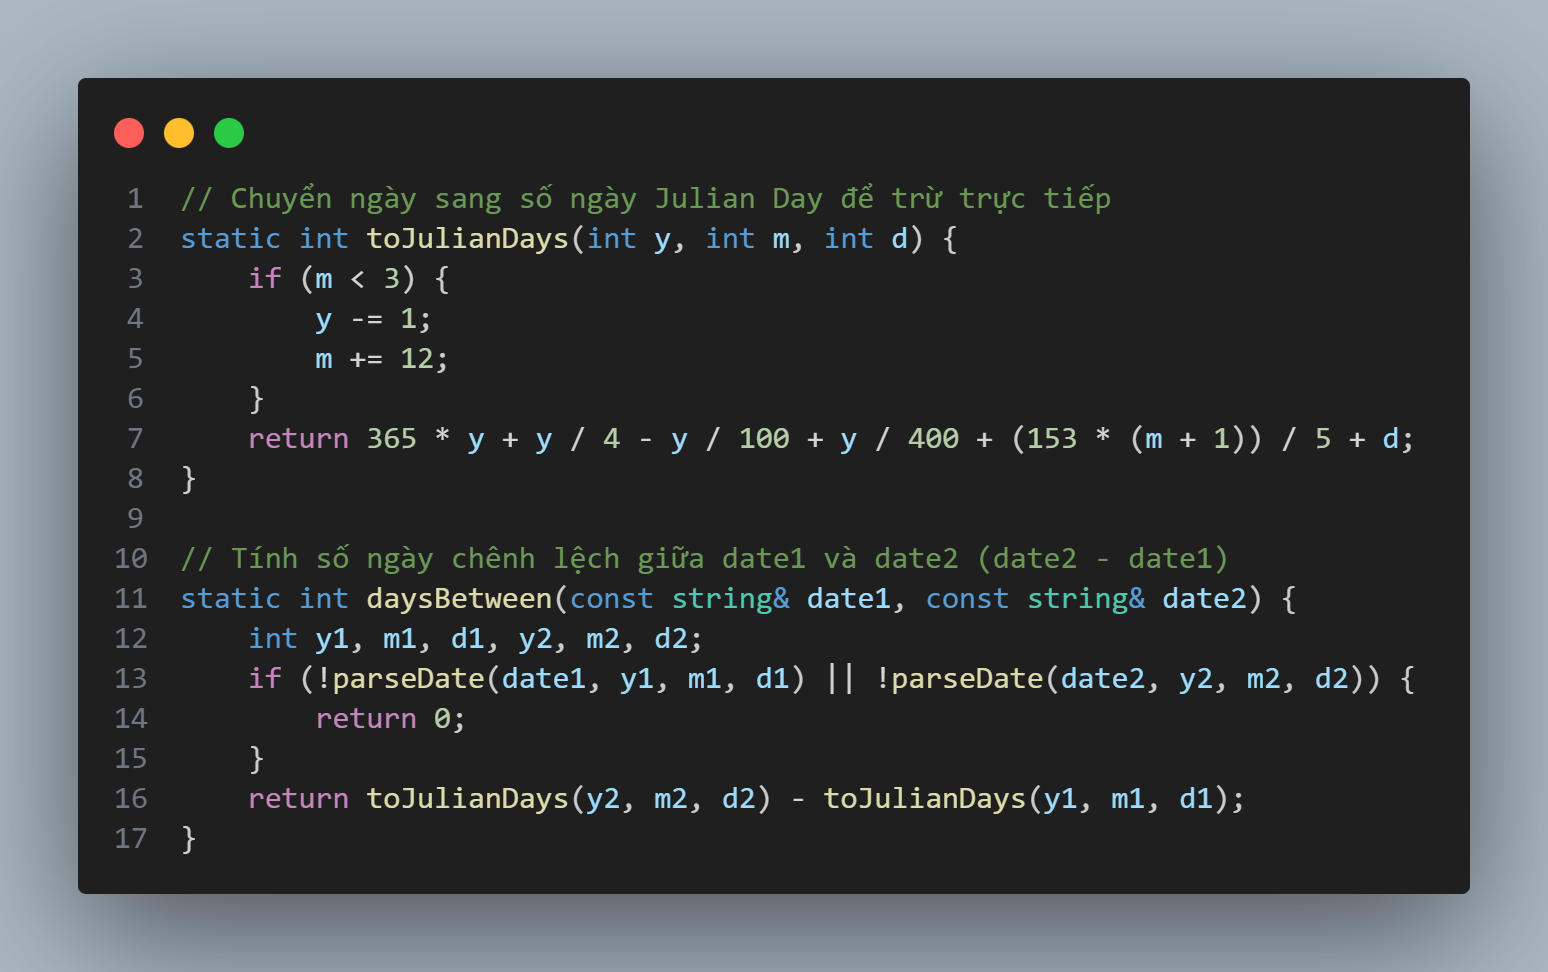
\includegraphics[width=0.88\linewidth]{code_date_utils_julian.png}
    \caption{Cài đặt thuật toán chuyển đổi Số ngày Julius trong lớp DateUtils}
    \label{fig:code_julian_date}
\end{figure}

Để tối ưu hóa triệt để thao tác này, nhóm đã cài đặt lớp tiện ích ngày tháng áp dụng thuật toán chuyển đổi mốc thời gian sang Số ngày Julius (Julian Day Number) như minh họa tại Hình \ref{fig:code_julian_date}. Thuật toán này ánh xạ một bộ ba năm, tháng, ngày thành một giá trị số nguyên duy nhất đại diện cho số ngày liên tục. Nhờ đó, việc so sánh hai mốc thời gian hay tính khoảng cách số ngày chênh lệch giữa ngày mượn và hạn trả được quy về phép trừ số nguyên đơn giản trong thời gian hằng số tức thời, loại bỏ hoàn toàn chi phí bóc tách chuỗi lặp đi lặp lại.

\subsection*{2.2. Hiện thực và phân tích chi tiết Module MC1: Tra cứu Mã Sách}
\addcontentsline{toc}{subsection}{2.2. Hiện thực và phân tích chi tiết Module MC1: Tra cứu Mã Sách}

\subsubsection*{2.2.1. Thuật toán Baseline: Tìm kiếm Tuần tự Tuyến tính $O(N)$}
\addcontentsline{toc}{subsubsection}{2.2.1. Thuật toán Baseline: Tìm kiếm Tuần tự Tuyến tính O(N)}

Thuật toán Baseline cho module tra cứu mã sách được hiện thực thông qua lớp tìm kiếm tuyến tính. Khi tiếp nhận một mã sách cần tra cứu, thuật toán sẽ duyệt tuần tự từ đầu đến cuối mảng danh sách sách, so sánh chuỗi mã sách cần tìm với mã sách của từng phần tử. Nếu tìm thấy phần tử trùng khớp, quá trình duyệt dừng lại và trả về kết quả; nếu duyệt hết mảng mà không thấy, thuật toán trả về trạng thái không tìm thấy.

Số phép so sánh chuỗi trong trường hợp xấu nhất bằng đúng tổng số lượng sách trong kho dữ liệu. Khi quy mô dữ liệu mở rộng lên hàng trăm nghìn bản ghi, thời gian thực thi tăng tỉ lệ thuận tuyến tính, tạo ra độ trễ đáng kể trong các thao tác vận hành thực tế.

\subsubsection*{2.2.2. Cấu trúc Tối ưu: Bảng băm Xích rời (Separate Chaining) \& Hàm băm DJB2}
\addcontentsline{toc}{subsubsection}{2.2.2. Cấu trúc Tối ưu: Bảng băm Xích rời (Separate Chaining) \& Hàm băm DJB2}

Để khắc phục hạn chế của phương pháp tuyến tính, giải pháp tối ưu sử dụng cấu trúc Bảng băm xích rời (Separate Chaining Hash Table) với kích thước bảng là một số nguyên tố lớn nhằm giảm thiểu tối đa hiện tượng va chạm khóa. Mỗi ô trong bảng băm lưu trữ một danh sách các bản ghi sách có cùng giá trị băm.

\begin{figure}[H]
    \centering
    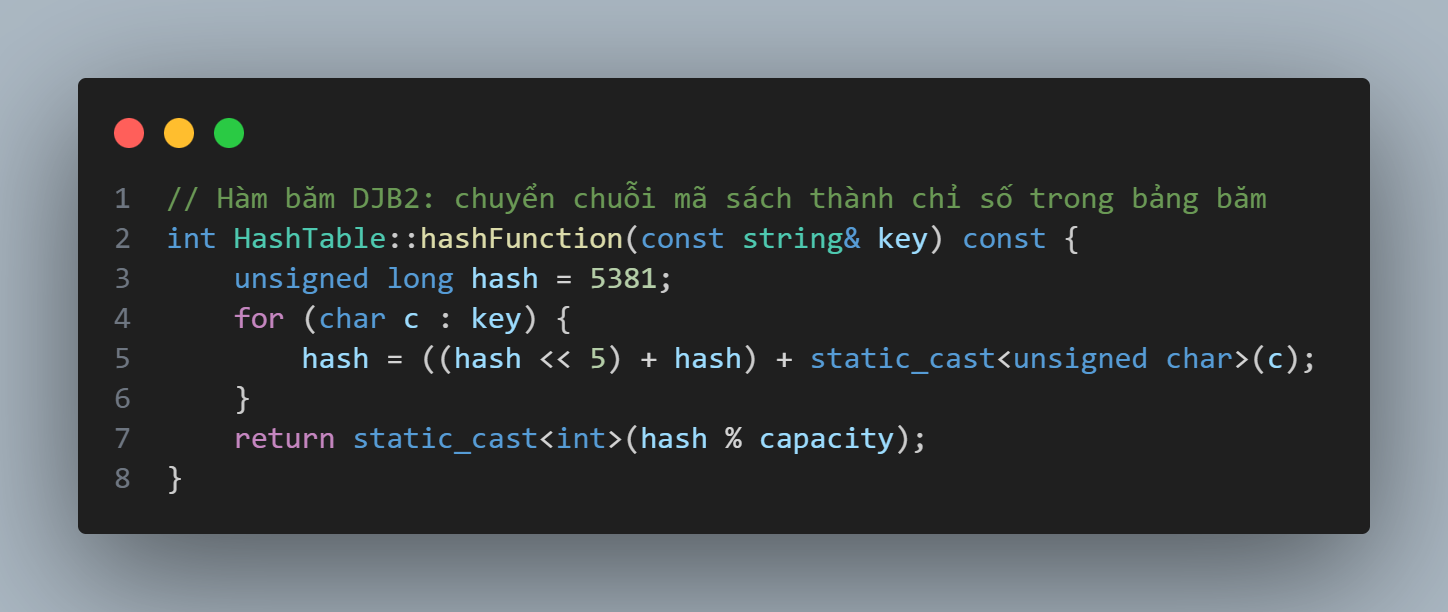
\includegraphics[width=0.88\linewidth]{code_mc1_hash_djb2.png}
    \caption{Hiện thực hàm băm chuỗi DJB2 cho cấu trúc Bảng băm MC1}
    \label{fig:code_mc1_djb2}
\end{figure}

Hàm băm được nhóm lựa chọn là thuật toán băm chuỗi kinh điển DJB2 do Daniel J. Bernstein thiết kế như thể hiện trong Hình \ref{fig:code_mc1_djb2}. Thuật toán này khởi tạo giá trị băm ban đầu và liên tục biến đổi qua từng ký tự của chuỗi mã sách bằng các phép dịch bit và phép cộng số học nhanh. Hàm DJB2 có khả năng phân tán các chuỗi ký tự có tiền tố tương đồng vào các ô băm cách xa nhau, đảm bảo hệ số tải của bảng luôn duy trì ở mức lý tưởng.

\subsubsection*{2.2.3. Tra cứu Bảng băm $O(1)$ \& Sơ đồ Tuần tự}
\addcontentsline{toc}{subsubsection}{2.2.3. Tra cứu Bảng băm O(1) \& Sơ đồ Tuần tự}

Khi thực hiện tra cứu mã sách, hệ thống tính toán giá trị băm của mã sách đầu vào để định vị chính xác ô chứa trong thời gian hằng số, sau đó chỉ duyệt qua một danh sách liên kết rất ngắn trong ô đó để lấy bản ghi.

\begin{figure}[H]
    \centering
    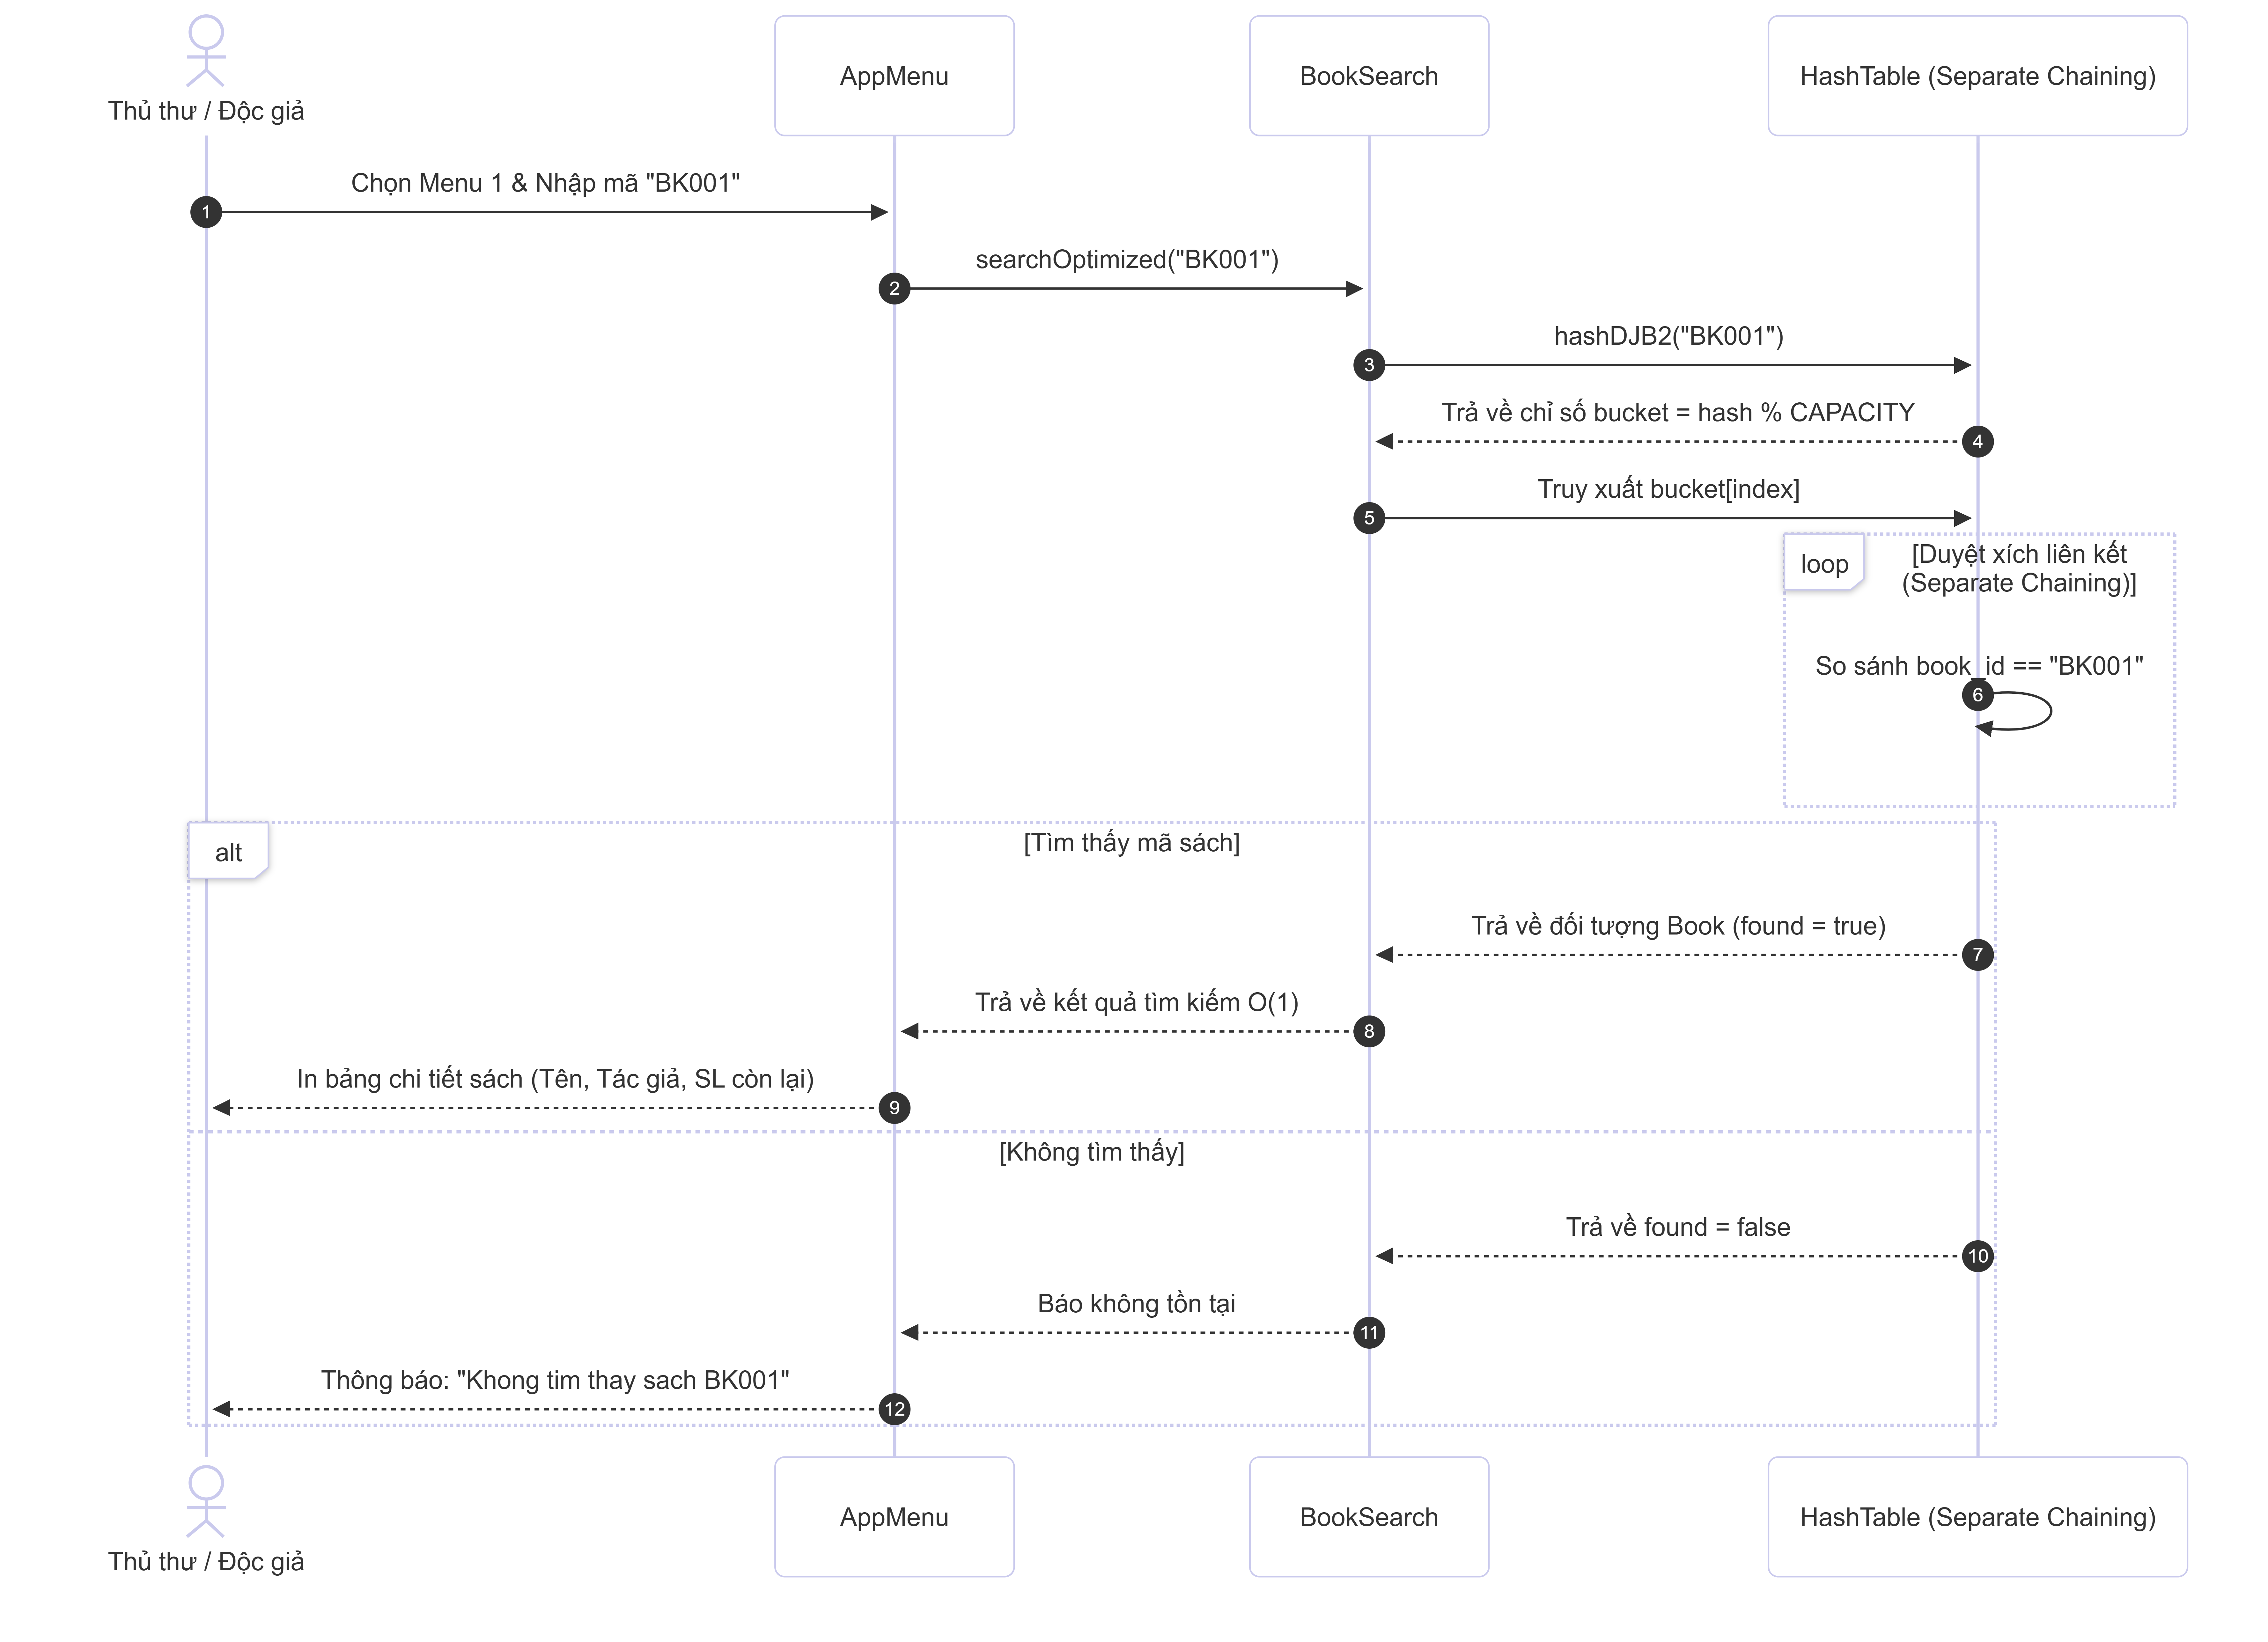
\includegraphics[width=0.85\linewidth]{seq_mc1_book_search.png}
    \caption{Sơ đồ tuần tự thể hiện luồng tra cứu sách theo mã định danh (MC1)}
    \label{fig:seq_mc1}
\end{figure}

Hình \ref{fig:seq_mc1} mô tả chi tiết luồng tương tác giữa người dùng, tầng Menu điều phối, thuật toán Baseline và giải pháp Bảng băm tối ưu. Trong chế độ đối sánh, hệ thống đồng thời đo đạc thời gian thực thi của cả hai phương pháp và kiểm định tính đồng nhất của kết quả tìm kiếm trước khi kết xuất ra màn hình.

\subsubsection*{2.2.4. Thực nghiệm kiểm chứng trên Giao diện dòng lệnh (CLI Validation)}
\addcontentsline{toc}{subsubsection}{2.2.4. Thực nghiệm kiểm chứng trên Giao diện dòng lệnh (CLI Validation)}

Để kiểm chứng sự hoạt động thực tế của Module MC1 trên môi trường thực thi, nhóm tiến hành chạy thử nghiệm trực tiếp trên giao diện dòng lệnh (TUI/CLI) với cả hai chế độ: Chế độ Vận hành thông thường (Normal Mode) và Chế độ Đối sánh thuật toán (Benchmark Mode).

Trong chế độ Normal Mode, người dùng nhập mã định danh tài liệu cần tra cứu (ví dụ \texttt{b001}) để hệ thống kích hoạt cơ chế băm và truy xuất tức thời thông tin chi tiết của đầu sách như thể hiện trong Hình \ref{fig:mc1_normal}.

\begin{figure}[H]
    \centering
    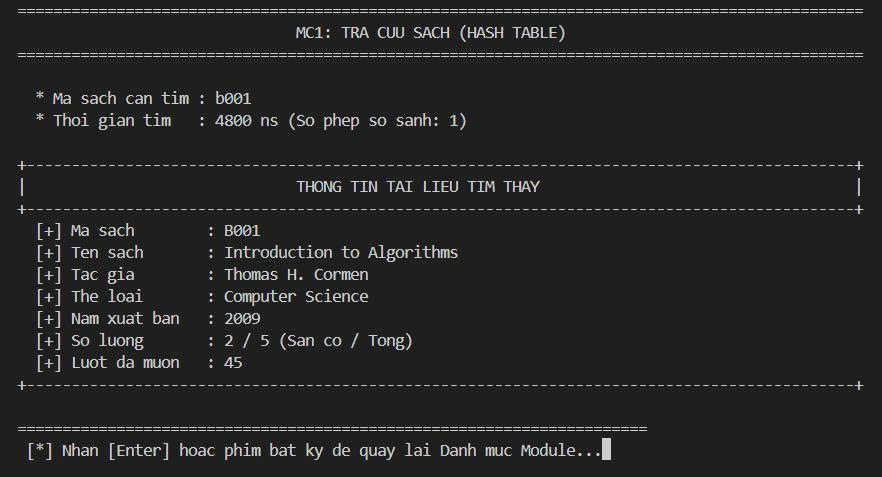
\includegraphics[width=0.78\linewidth]{mc1_normal_view.jpg}
    \caption{Giao diện tra cứu thông tin sách theo mã định danh bằng Hash Table (Normal Mode)}
    \label{fig:mc1_normal}
\end{figure}

Kết quả hiển thị trên Hình \ref{fig:mc1_normal} cho thấy hệ thống trả về đầy đủ và chính xác các trường thuộc tính của cuốn sách tương ứng: Mã sách \texttt{B001}, Tên sách \textit{Introduction to Algorithms}, Tác giả \textit{Thomas H. Cormen}, Thể loại \textit{Computer Science}, Năm xuất bản \textit{2009}, Số lượng sẵn có \textit{2/5} và Tổng số lượt đã mượn \textit{45}. Quá trình tra cứu chỉ tiêu tốn duy nhất $1$ phép so sánh khóa tại ô băm mục tiêu, phản ánh đúng đặc tính truy xuất trực tiếp của cấu trúc Bảng băm.

Tiếp theo, hệ thống được chuyển sang chế độ Benchmark Mode nhằm đối chiếu trực tiếp giữa thuật toán Baseline (Linear Search) và cấu trúc tối ưu (Separate Chaining Hash Table) trong trường hợp mã sách tồn tại trong kho dữ liệu (Hình \ref{fig:mc1_found}).

\begin{figure}[H]
    \centering
    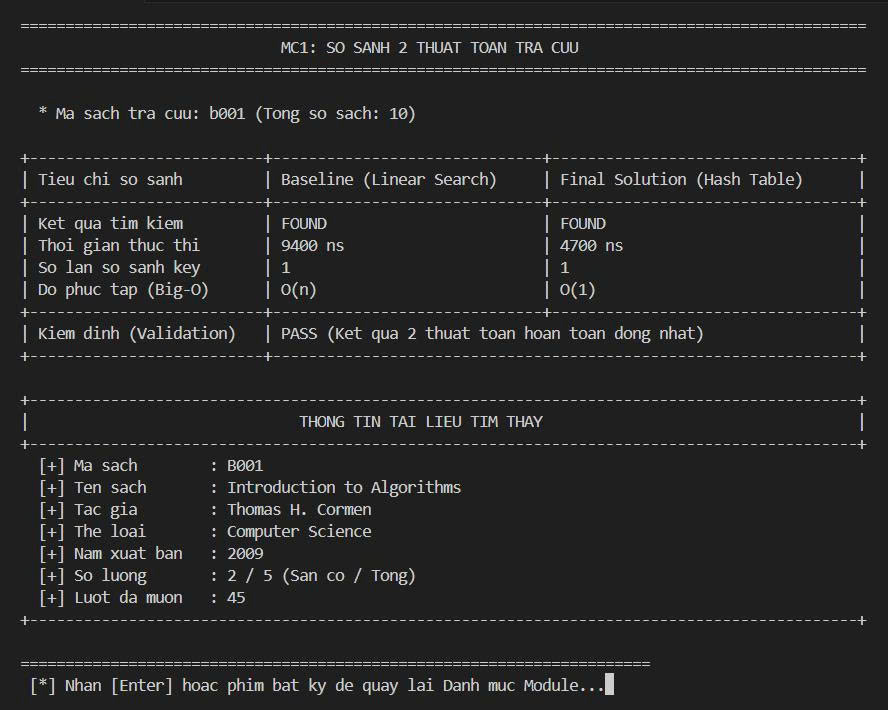
\includegraphics[width=0.76\linewidth]{mc1_benchmark_found.jpg}
    \caption{Đối sánh thực nghiệm giữa Linear Search và Hash Table khi tìm thấy mã sách}
    \label{fig:mc1_found}
\end{figure}

Từ kết quả đối sánh tại Hình \ref{fig:mc1_found}, cả hai phương pháp đều trả về trạng thái \texttt{FOUND} với đúng bản ghi \texttt{B001}, giúp chương trình ghi nhận trạng thái kiểm định \texttt{PASS (Ket qua 2 thuat toan hoan toan dong nhat)}. Ở lần chạy minh họa cụ thể này, thời gian ghi nhận của Hash Table là $4.700\text{ ns}$ so với $9.400\text{ ns}$ của Linear Search. Cần lưu ý rằng giá trị thời gian trong ảnh chụp chỉ mang tính chất minh chứng cho một lần thực thi trực quan; hiệu năng trung bình toàn diện sẽ được tổng hợp khoa học qua hàng nghìn chu kỳ lặp ở Bảng \ref{tab:benchmark_n10}.

Đối với trường hợp kiểm thử biên khi người dùng nhập một mã sách không tồn tại trong hệ thống (ví dụ \texttt{b9999}), việc đánh giá hành vi của hai thuật toán mang ý nghĩa lý thuyết rất quan trọng (Hình \ref{fig:mc1_notfound}).

\begin{figure}[H]
    \centering
    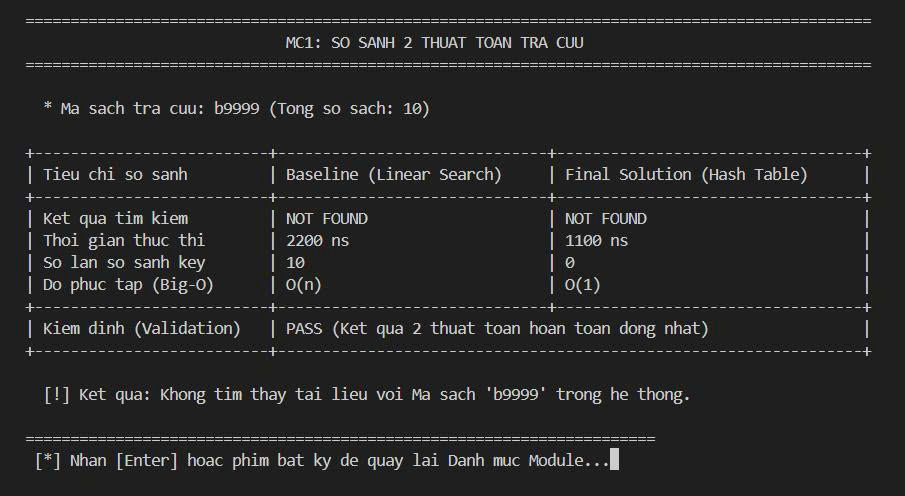
\includegraphics[width=0.78\linewidth]{mc1_benchmark_notfound.jpg}
    \caption{Đối sánh thực nghiệm giữa Linear Search và Hash Table khi mã sách không tồn tại}
    \label{fig:mc1_notfound}
\end{figure}

Khi mã sách không tồn tại trong kho $N=10$ phần tử, thuật toán Linear Search rơi vào kịch bản xấu nhất khi buộc phải duyệt tuần tự qua toàn bộ $10$ phần tử trong mảng ($10$ phép so sánh) mới có thể kết luận không tìm thấy. Ngược lại, cấu trúc Hash Table tính toán giá trị băm của \texttt{b9999}, ánh xạ đến một ô băm rỗng và lập tức trả về \texttt{NOT FOUND} với $0$ phép so sánh chuỗi, bảo toàn chi phí thời gian ở mức hằng số $O(1)$. Trạng thái kiểm định đạt \texttt{PASS}, xác nhận tính nhất quán tuyệt đối về mặt logic đầu ra giữa hai phương pháp.

Sau khi kiểm chứng tính đúng đắn và hành vi cơ bản của hai thuật toán trên môi trường dòng lệnh (CLI), hệ thống tiếp tục mở rộng quy mô dữ liệu lên mức xấp xỉ $500.000$ đầu sách được nạp toàn phần vào bộ nhớ RAM trên nền tảng DSA Performance Dashboard (Web) nhằm quan sát rõ nét đặc tính hiệu năng khi kích thước dữ liệu tăng vọt.

\begin{figure}[H]
    \centering
    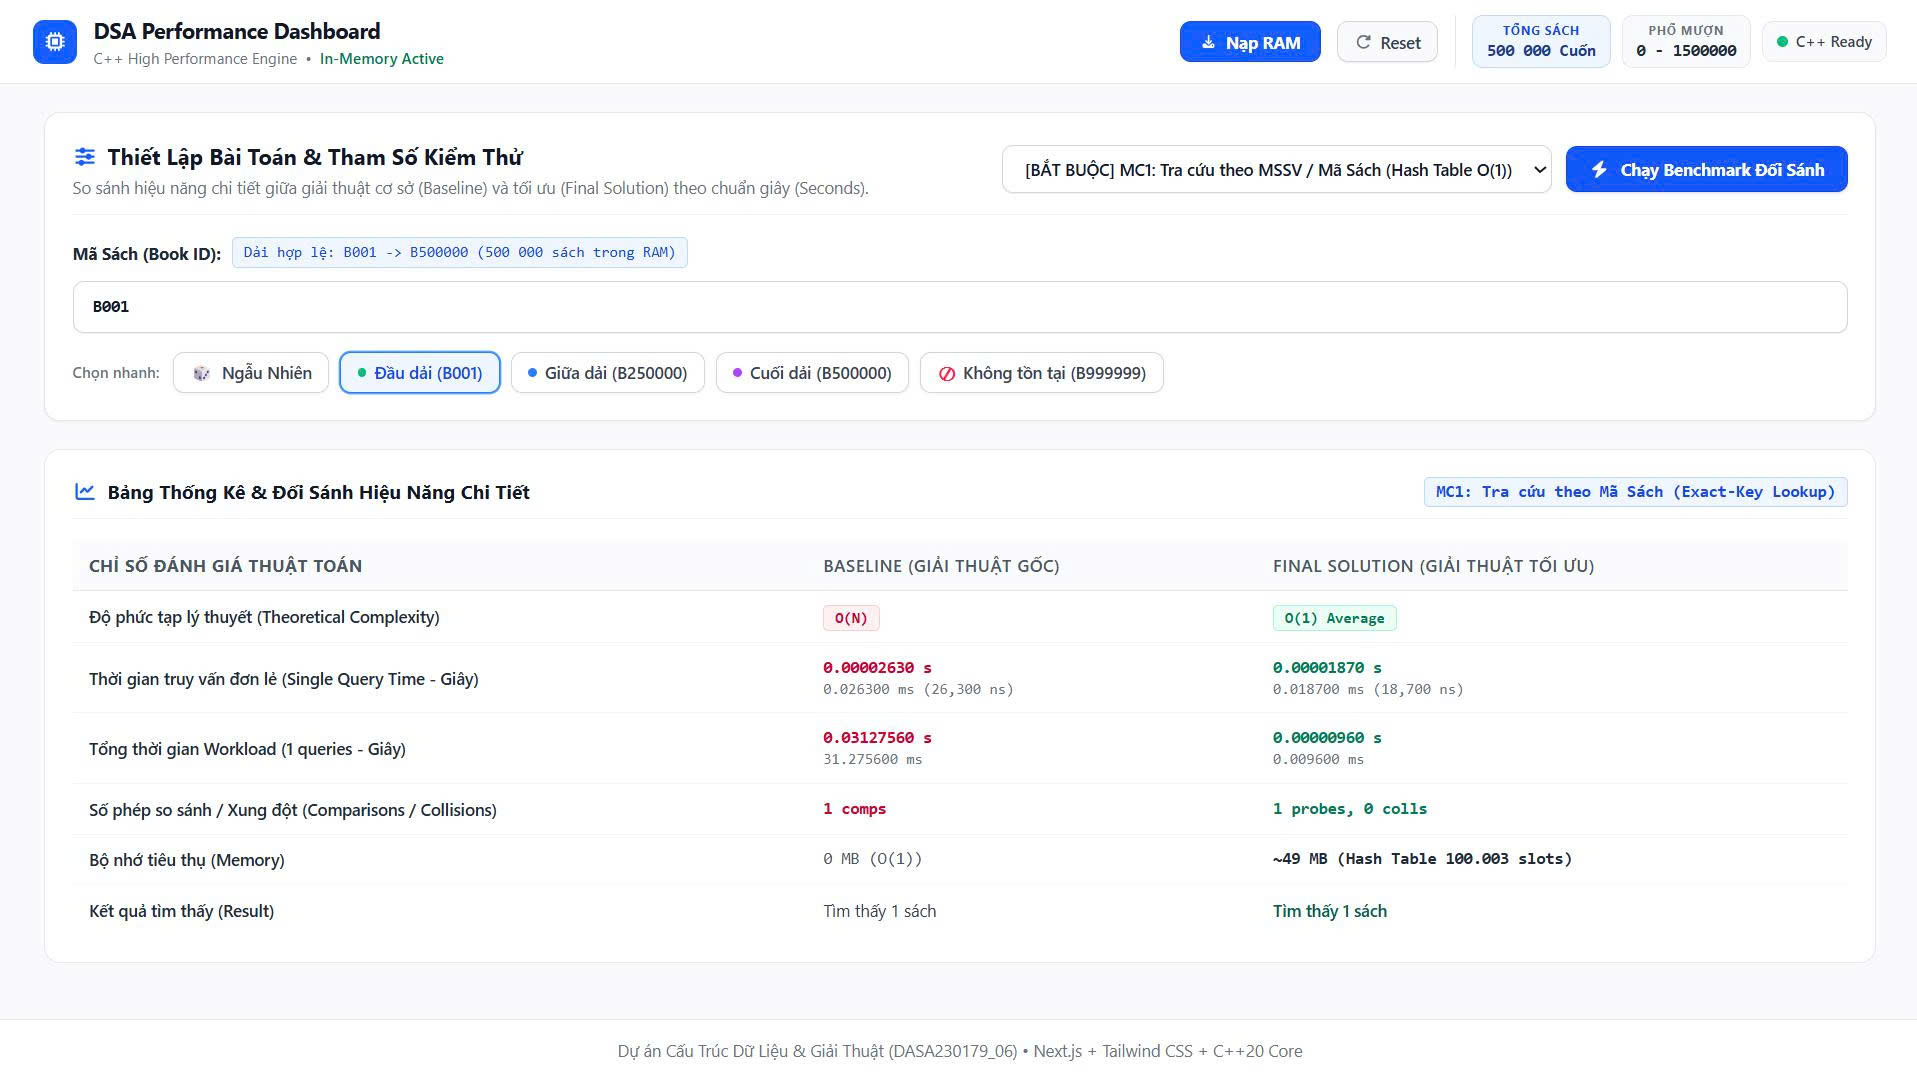
\includegraphics[width=0.88\linewidth]{mc1_benchmark_head_B001.jpg}
    \caption{Benchmark MC1 với mã sách ở đầu tập dữ liệu (B001)}
    \label{fig:web-mc1-head}
\end{figure}

Trong lần chạy thử nghiệm với mã sách nằm ngay đầu tập dữ liệu (\texttt{B001}) như thể hiện ở Hình \ref{fig:web-mc1-head}, thuật toán Linear Search tìm thấy kết quả ngay tại phần tử đầu tiên với đúng $1$ phép so sánh, ghi nhận thời gian truy vấn đơn lẻ là $0.026\text{ ms}$. Cấu trúc Hash Table thực hiện hàm băm DJB2 và truy cập trực tiếp ô băm với $1$ probe, $0$ va chạm, ghi nhận thời gian $0.018\text{ ms}$. Cả hai giải pháp đều trả về đúng $1$ bản ghi khớp (PASS). Trường hợp này là kịch bản thuận lợi nhất cho tìm kiếm tuần tự ($O(1)$), do đó không thể đại diện cho hiệu năng tổng thể của hệ thống khi dữ liệu mở rộng.

\begin{figure}[H]
    \centering
    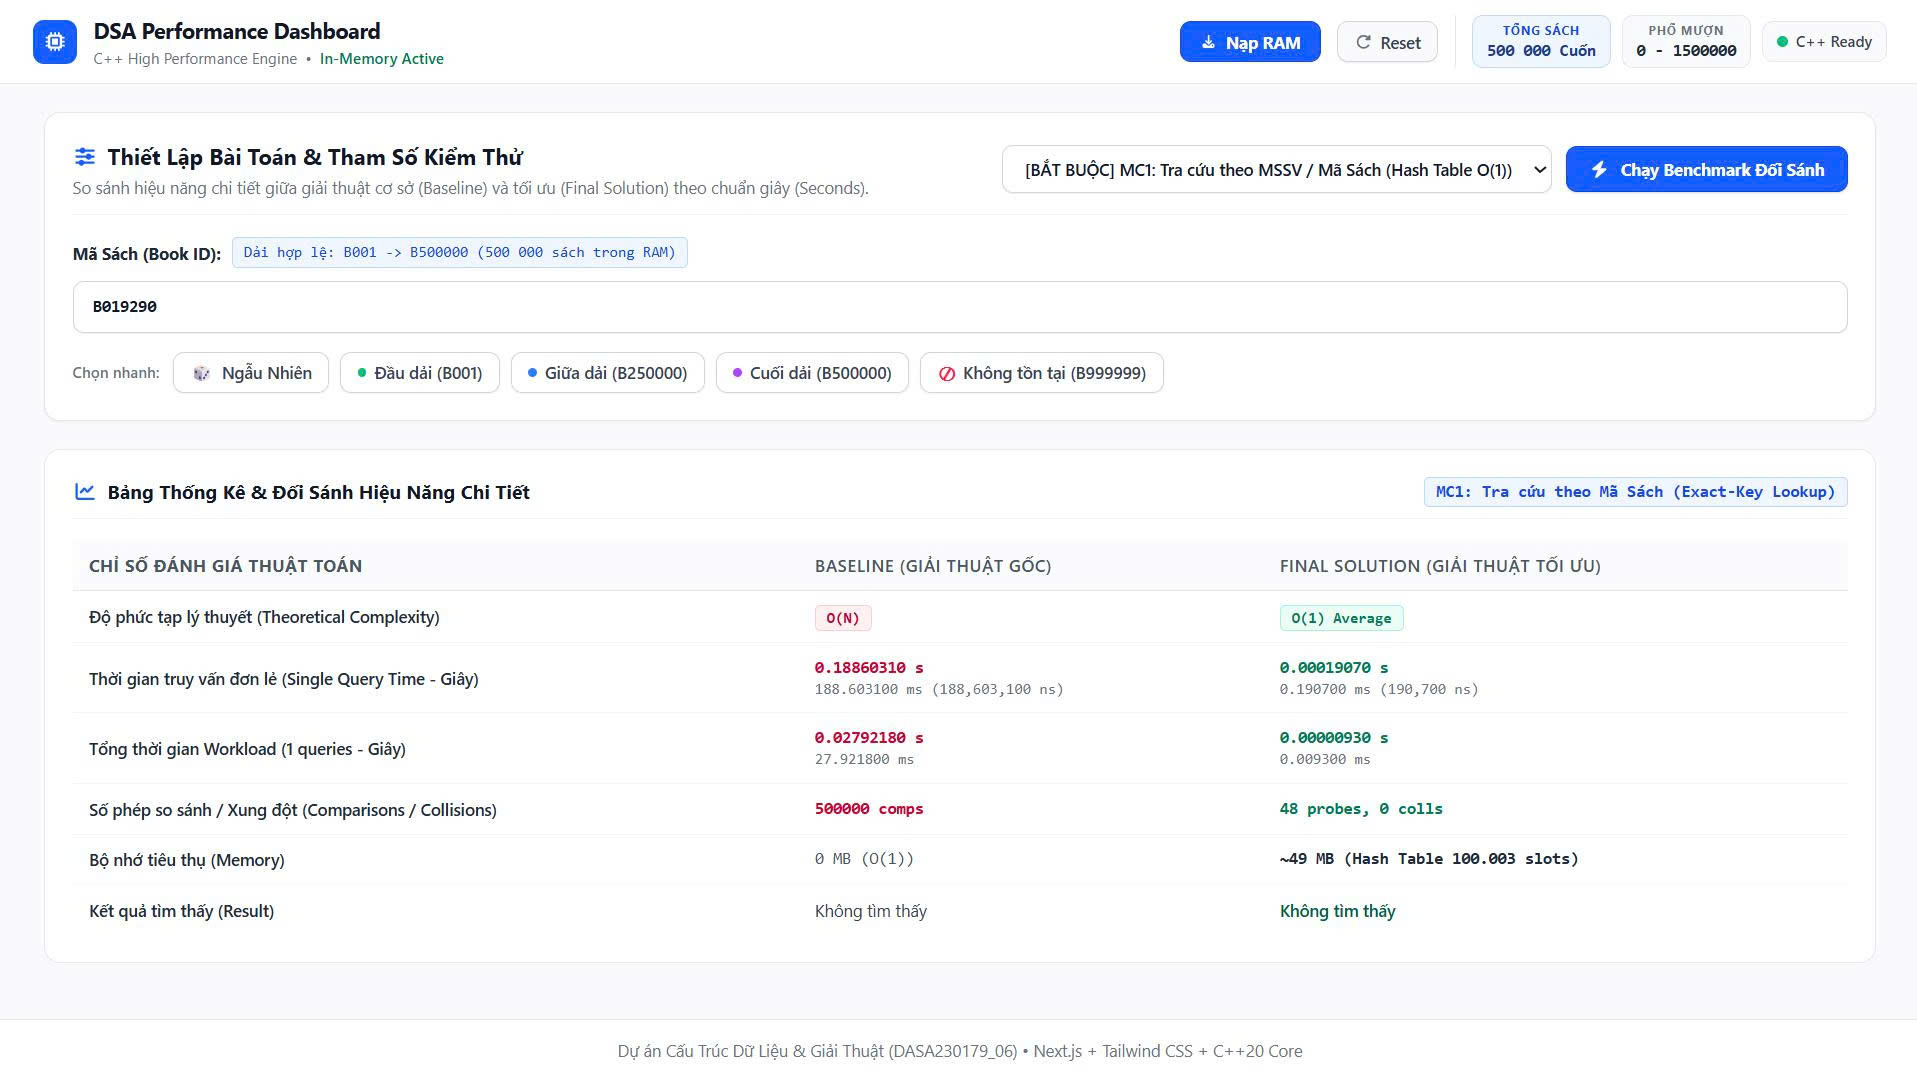
\includegraphics[width=0.88\linewidth]{mc1_benchmark_random.jpg}
    \caption{Benchmark MC1 với mã sách ngẫu nhiên (B019290)}
    \label{fig:web-mc1-random}
\end{figure}

Tiếp theo, thử nghiệm với một mã sách ngẫu nhiên \texttt{B019290} (Hình \ref{fig:web-mc1-random}) nhằm khảo sát hành vi truy xuất ngoài các vị trí biên. Tại lần đo này, Linear Search phải duyệt qua toàn bộ $500.000$ phần tử ($188.6\text{ ms}$) trước khi kết luận không tìm thấy, trong khi Hash Table thực hiện $48$ probes ($0.190\text{ ms}$) để xác nhận ô băm rỗng, cùng trả về kết quả $0$ sách khớp (PASS). Kết quả này cho thấy sự khác biệt rõ rệt khi truy vấn không nằm ở vị trí đầu dãy.

\begin{figure}[H]
    \centering
    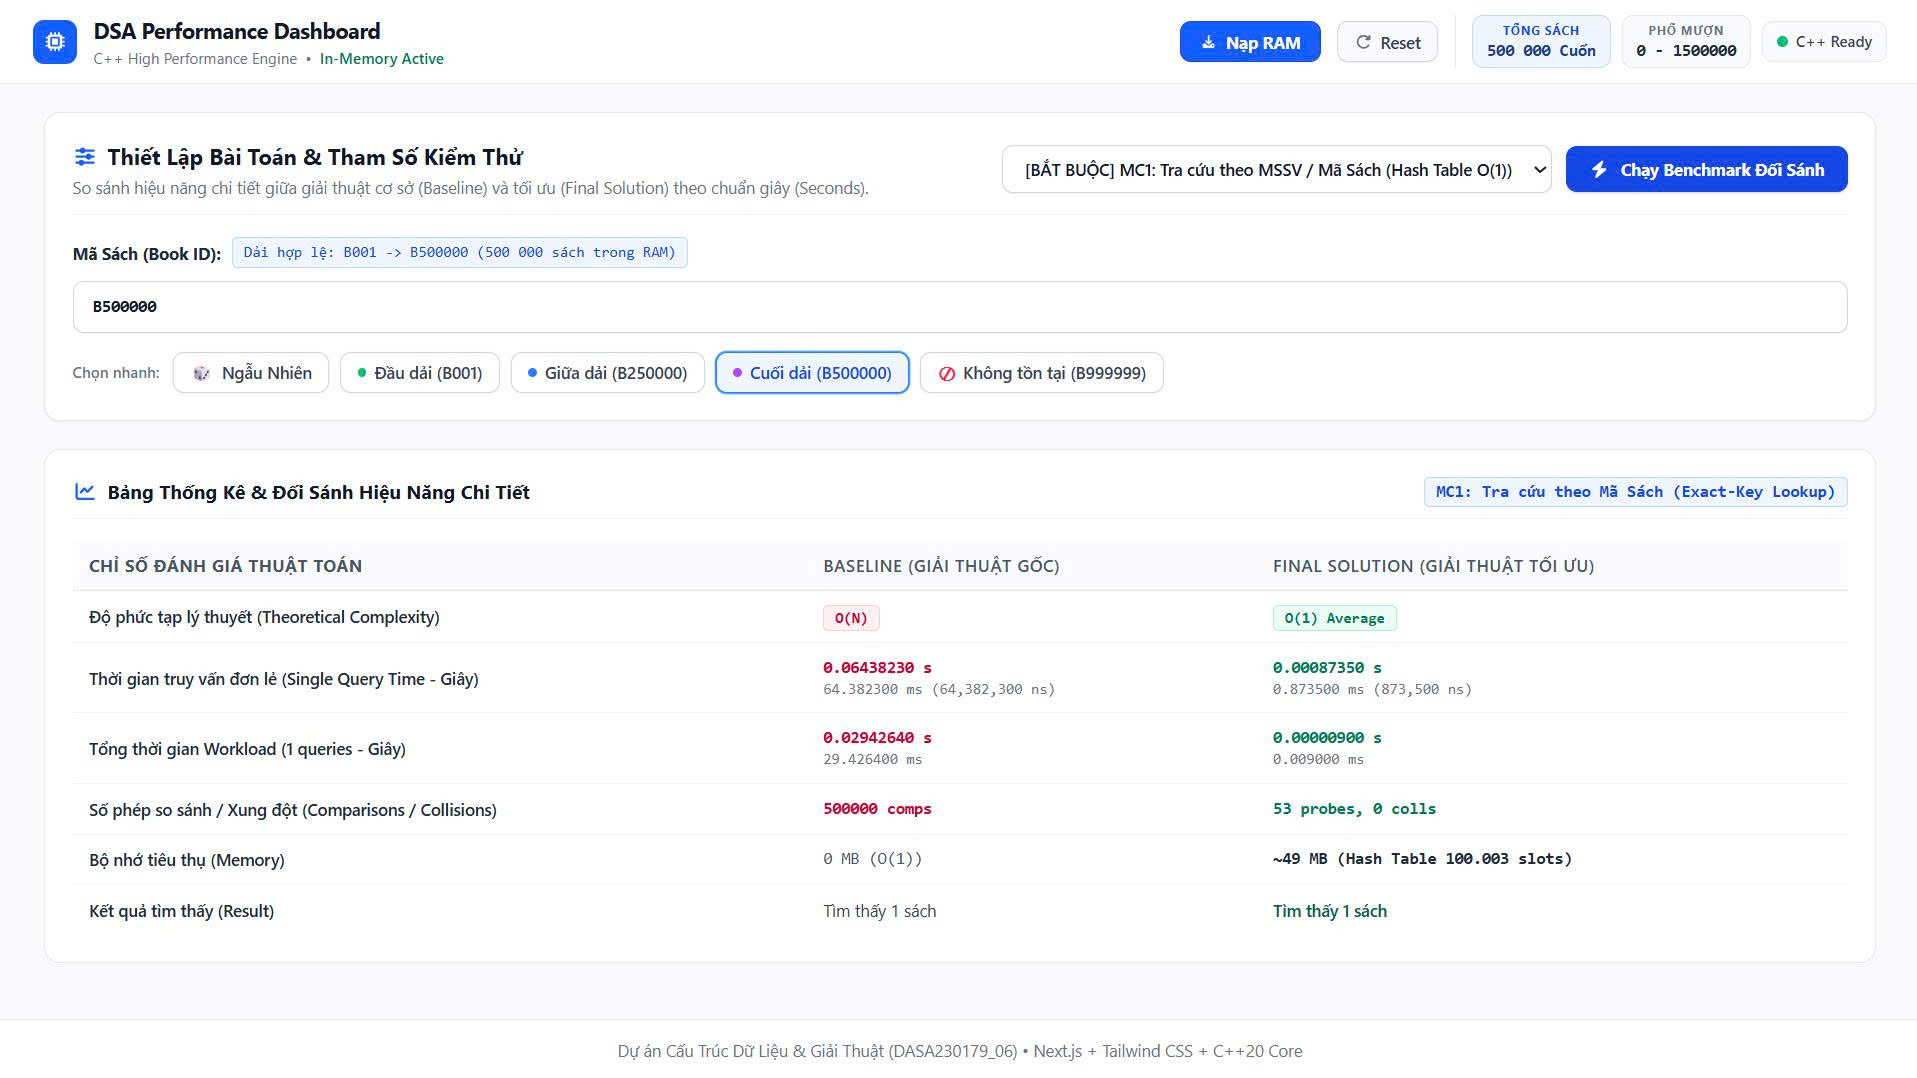
\includegraphics[width=0.88\linewidth]{mc1_benchmark_tail_B500000.jpg}
    \caption{Benchmark MC1 với mã sách ở cuối tập dữ liệu (B500000)}
    \label{fig:web-mc1-tail}
\end{figure}

Ở kịch bản kiểm thử với mã sách nằm ở cuối tập dữ liệu (\texttt{B500000}) tại Hình \ref{fig:web-mc1-tail}, Linear Search phải duyệt qua $500.000$ phần tử trên bộ nhớ chính với thời gian $64.38\text{ ms}$. Ngược lại, Hash Table tính toán giá trị băm và định vị thành công bản ghi với $53$ probes, $0$ va chạm trong $0.873\text{ ms}$, trả về chính xác cùng một bản ghi \texttt{B500000} (PASS). Đây là trường hợp làm bộc lộ rõ hạn chế nghiêm trọng của quét tuyến tính khi phần tử cần tìm nằm ở cuối không gian lưu trữ.

\begin{figure}[H]
    \centering
    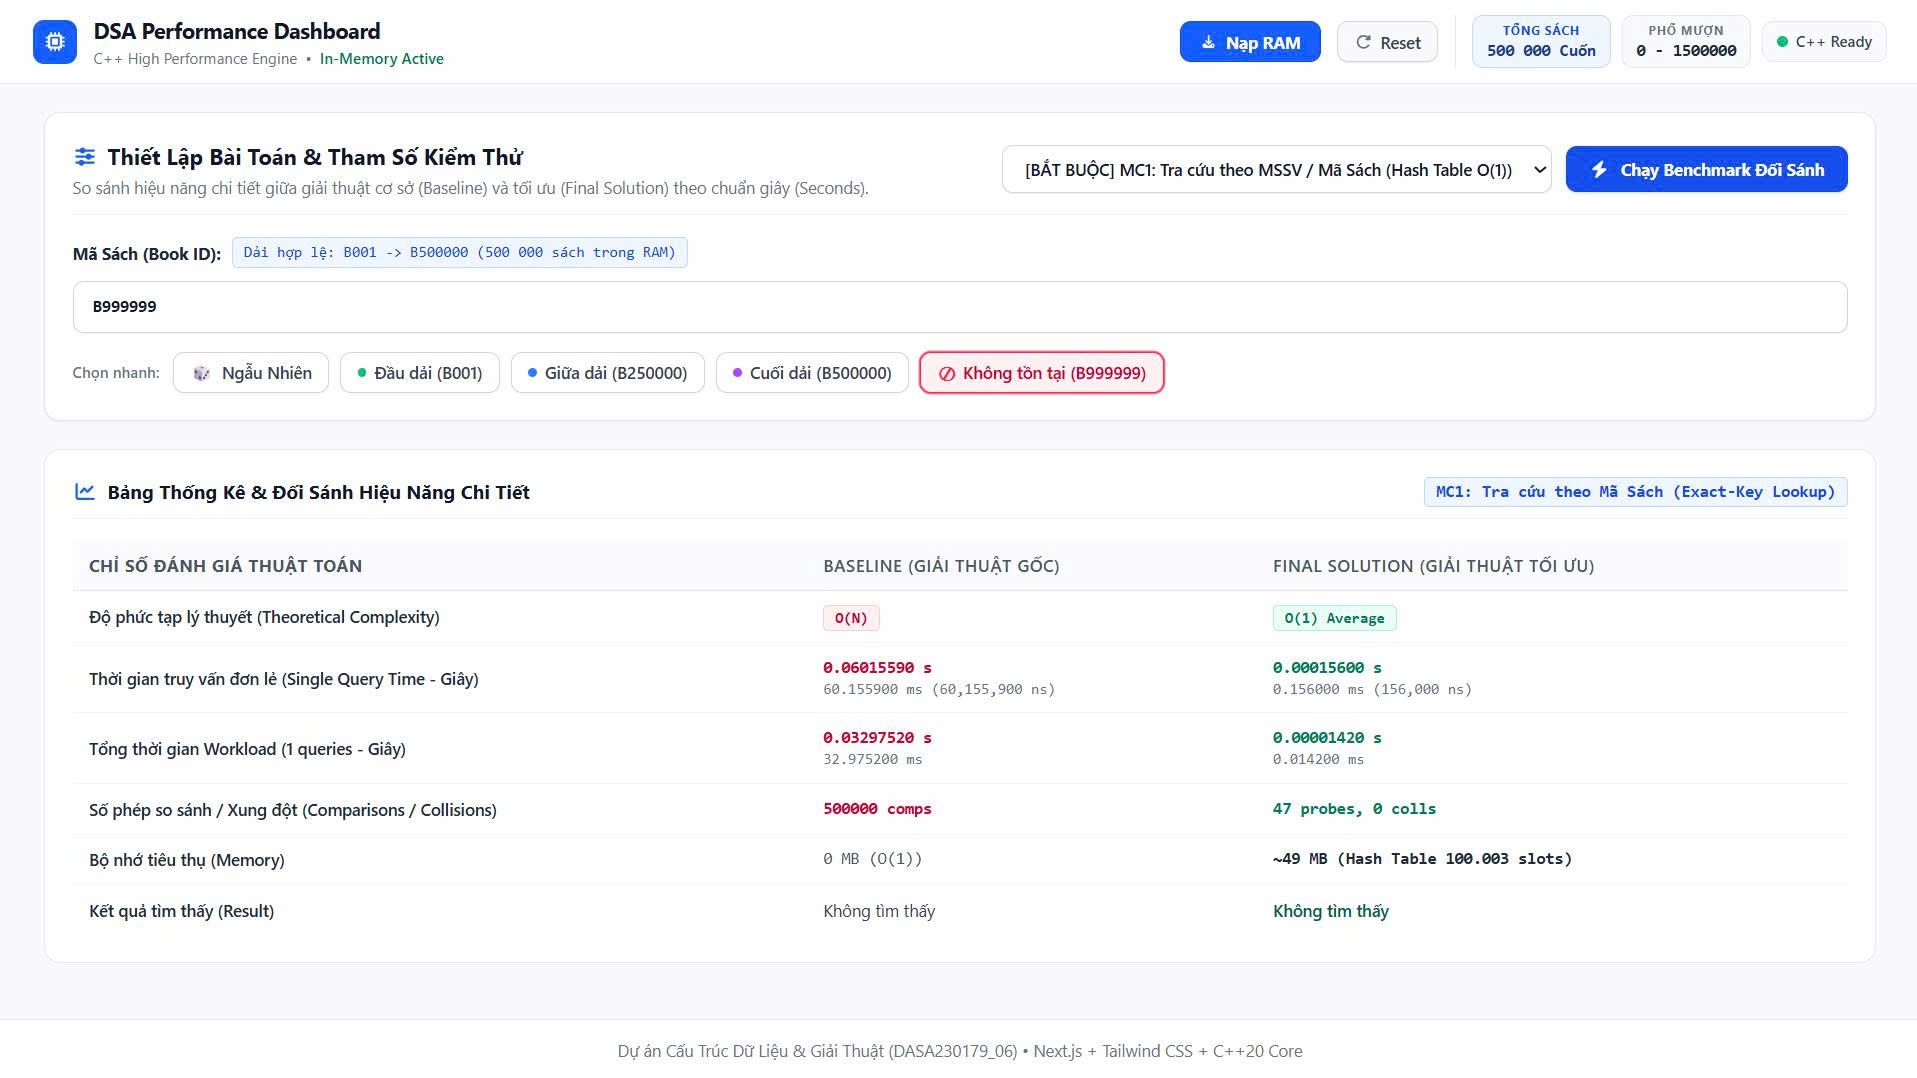
\includegraphics[width=0.88\linewidth]{mc1_benchmark_not_found_B999999.jpg}
    \caption{Benchmark MC1 trong trường hợp mã sách không tồn tại (B999999)}
    \label{fig:web-mc1-notfound}
\end{figure}

Đối với truy vấn phủ định (negative lookup) khi mã sách hoàn toàn không tồn tại (\texttt{B999999}) ở Hình \ref{fig:web-mc1-notfound}, Linear Search bắt buộc phải quét toàn bộ $500.000$ cuốn sách ($60.15\text{ ms}$) mới có thể đưa ra kết luận. Hash Table chỉ cần thực hiện $47$ probes ($0.156\text{ ms}$) tại ô băm tương ứng và lập tức xác nhận không tìm thấy (PASS).

Tổng hợp đánh giá Module MC1: Tổng thể 4 kịch bản benchmark trên tập $500.000$ bản ghi chứng minh rằng hiệu năng của Linear Search phụ thuộc chặt chẽ vào vị trí vật lý và sự tồn tại của phần tử trong mảng dữ liệu. Ngược lại, Bảng băm tiếp cận dữ liệu dựa trên giá trị khóa băm, duy trì số phép thăm dò ở mức rất nhỏ. Về mặt đánh đổi tài nguyên (Trade-off), Bảng băm đòi hỏi dung lượng bộ nhớ phụ xấp xỉ $48.74\text{ MB}$ để duy trì $100.003$ bucket và các con trỏ liên kết, đổi lại hệ thống đạt được tốc độ phản hồi tức thì và ổn định ở mọi vị trí khóa.

\subsection*{2.3. Hiện thực và phân tích chi tiết Module MC2: Top Sách Mượn Nhiều Nhất}
\addcontentsline{toc}{subsection}{2.3. Hiện thực và phân tích chi tiết Module MC2: Top Sách Mượn Nhiều Nhất}

\subsubsection*{2.3.1. Thuật toán Baseline: Quét Tuyến tính Tìm Cực đại $O(N \cdot K)$}
\addcontentsline{toc}{subsubsection}{2.3.1. Thuật toán Baseline: Quét Tuyến tính Tìm Cực đại O(N * K)}

Thuật toán Baseline cho bài toán xác định sách có lượt mượn nhiều nhất được hiện thực bằng cách quét tuyến tính toàn bộ danh sách sách để tìm phần tử có trường lượt mượn lớn nhất. Trong mỗi lần quét, thuật toán duy trì một biến tạm lưu trữ chỉ số cuốn sách có lượt mượn cao nhất từng thấy và so sánh lần lượt với tất cả các phần tử còn lại.

Phương pháp này tiêu tốn số phép so sánh tỉ lệ thuận với kích thước kho sách cho mỗi lần truy vấn. Khi cần truy xuất nhiều lần trong ngày hoặc lấy danh sách các đầu sách dẫn đầu, chi phí quét lặp đi lặp lại trên toàn bộ mảng dữ liệu trở thành một điểm nghẽn nghiêm trọng của hệ thống.

\subsubsection*{2.3.2. Cấu trúc Tối ưu: Max-Heap \& Thuật toán Floyd Bottom-Up $O(N)$}
\addcontentsline{toc}{subsubsection}{2.3.2. Cấu trúc Tối ưu: Max-Heap \& Thuật toán Floyd Bottom-Up O(N)}

Giải pháp tối ưu xây dựng một Cây đống cực đại (Max-Heap) hoàn chỉnh được lưu trữ trực tiếp trên một mảng động liền mạch. Cây đống duy trì bất biến cấu trúc: giá trị số lượt mượn của mỗi nút cha luôn lớn hơn hoặc bằng giá trị lượt mượn của hai nút con.

\begin{figure}[H]
    \centering
    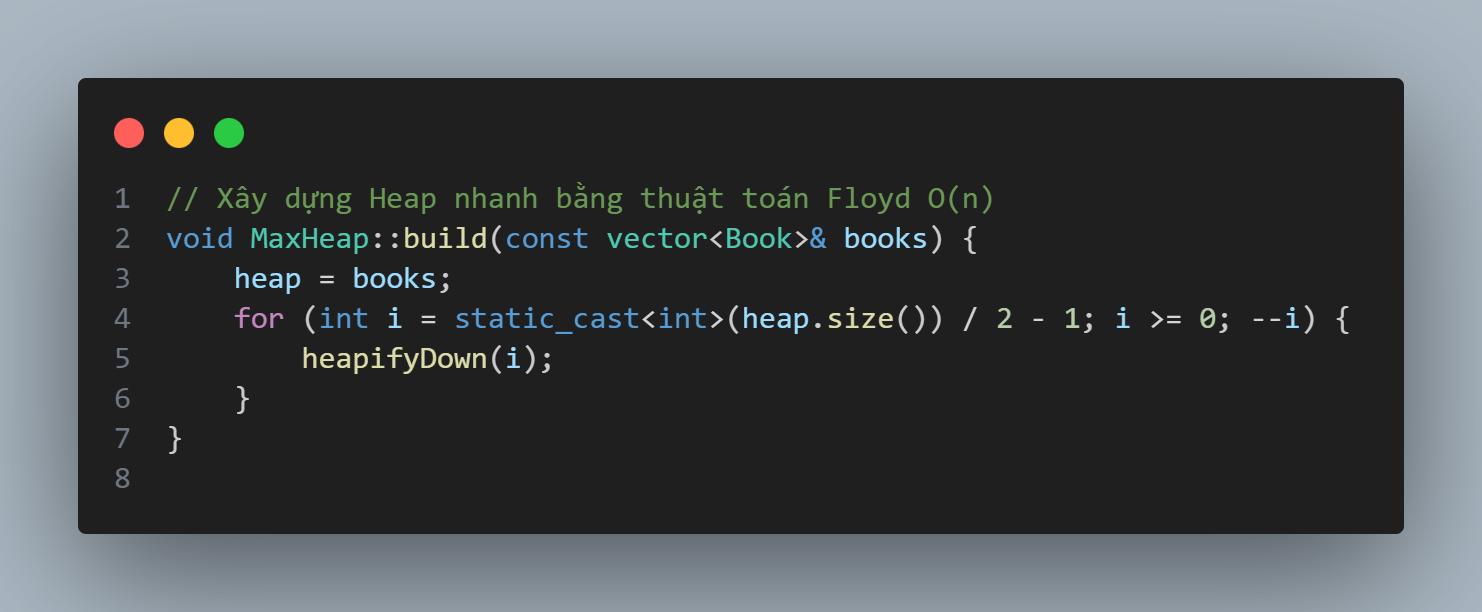
\includegraphics[width=0.85\linewidth]{code_mc2_floyd_build.png}
    \caption{Hiện thực thuật toán xây dựng Max-Heap từ dưới lên theo nguyên lý Floyd}
    \label{fig:code_mc2_floyd}
\end{figure}

Khi nạp toàn bộ danh sách sách vào đống, thay vì chèn từng phần tử, nhóm áp dụng thuật toán xây dựng đống từ dưới lên của Floyd như thể hiện ở Hình \ref{fig:code_mc2_floyd}. Thuật toán bắt đầu từ các nút nội tại ở nửa dưới mảng và liên tục sàng phần tử xuống dưới để thỏa mãn tính chất đống. Phương pháp này cho phép kiến tạo toàn bộ cây đống với tổng số phép toán tỉ lệ thuận tuyến tính theo số phần tử, vượt trội hơn hẳn cách chèn tuần tự từng phần tử.

\subsubsection*{2.3.3. Trích xuất Top-$K$ Cực trị $O(1) / O(K \log N)$ \& Sơ đồ Tuần tự}
\addcontentsline{toc}{subsubsection}{2.3.3. Trích xuất Top-K Cực trị O(1) / O(K log N) \& Sơ đồ Tuần tự}

Sau khi cấu trúc đống được thiết lập, phần tử có số lượt mượn cao nhất luôn nằm tại vị trí đầu tiên của mảng. Thao tác lấy phần tử cực đại diễn ra tức thời trong thời gian hằng số mà không cần bất kỳ phép so sánh nào trên phần còn lại của tập dữ liệu.

\begin{figure}[H]
    \centering
    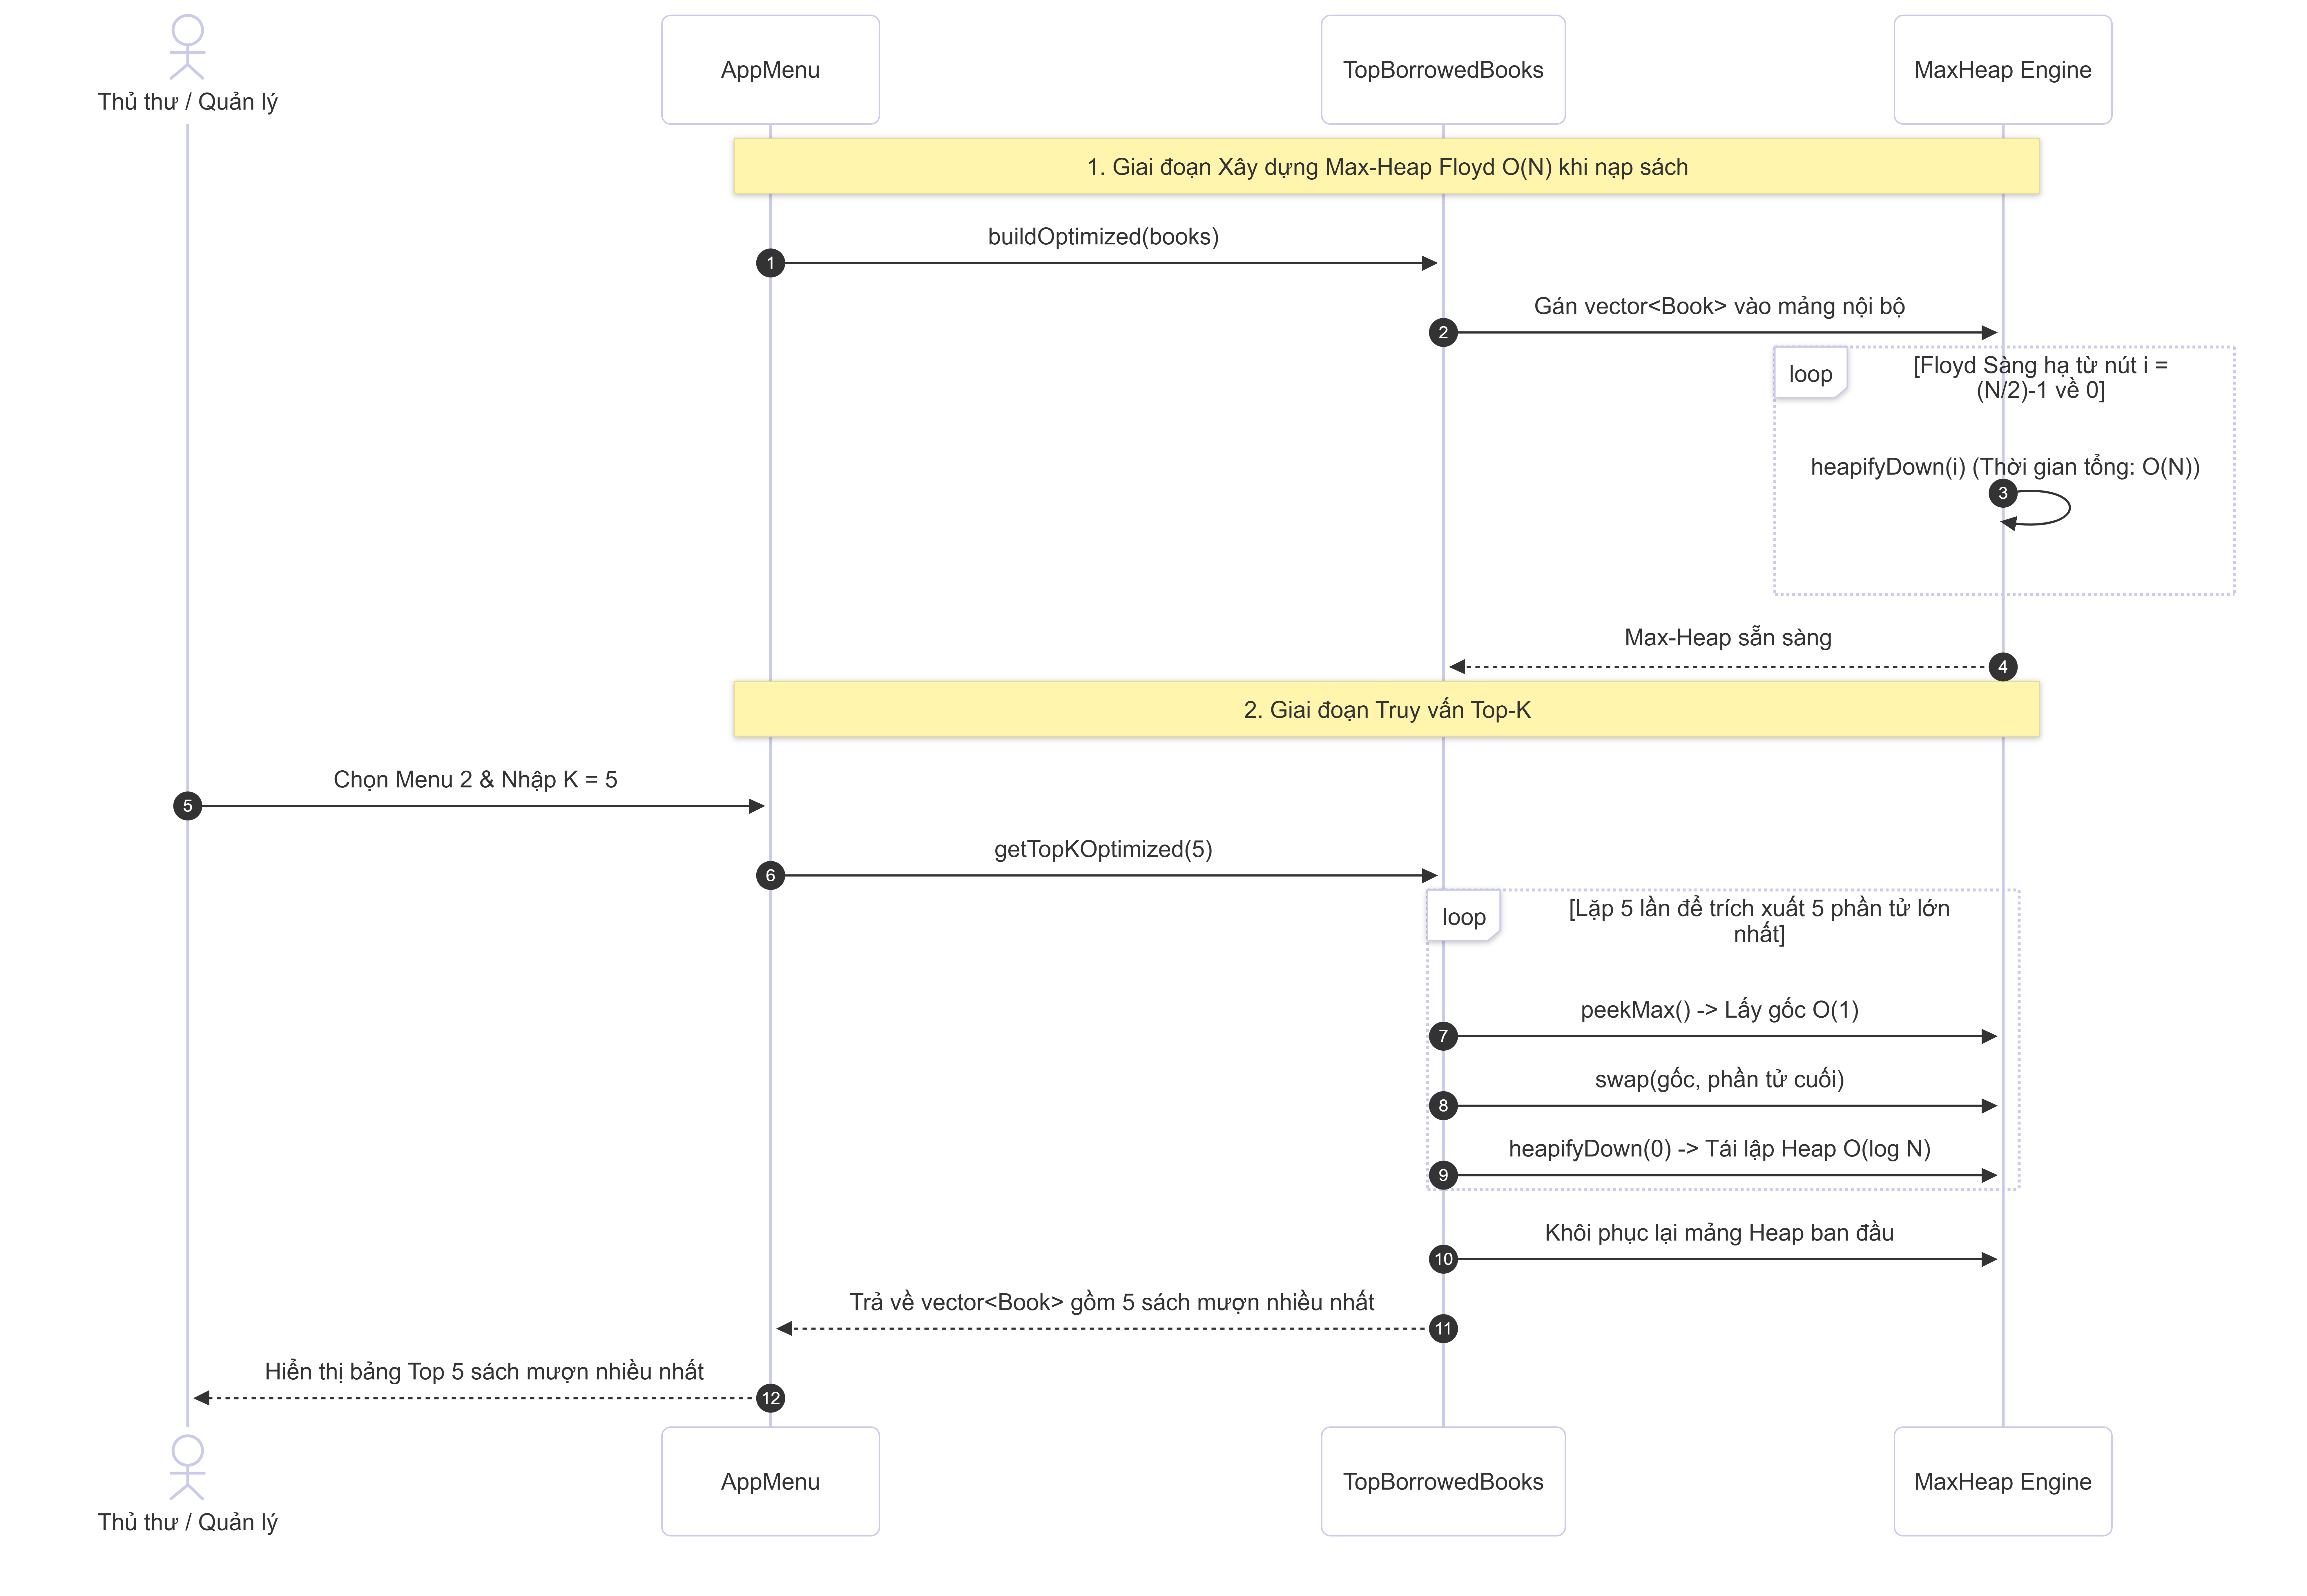
\includegraphics[width=0.82\linewidth]{seq_mc2_top_borrowed_heap.png}
    \caption{Sơ đồ tuần tự thể hiện luồng trích xuất sách mượn nhiều nhất (MC2)}
    \label{fig:seq_mc2}
\end{figure}

Luồng thực thi hoàn chỉnh của module MC2 được trình bày trên sơ đồ tuần tự tại Hình \ref{fig:seq_mc2}. Khi có một độc giả mượn sách mới, hàm cập nhật số lượt mượn sẽ điều chỉnh giá trị của cuốn sách và thực hiện thao tác sàng lên phía gốc trong thời gian logarit theo chiều cao đống, bảo đảm hệ thống luôn trong trạng thái sẵn sàng cung cấp kết quả cực trị.

\subsubsection*{2.3.4. Thực nghiệm kiểm chứng trên Giao diện dòng lệnh (CLI Validation)}
\addcontentsline{toc}{subsubsection}{2.3.4. Thực nghiệm kiểm chứng trên Giao diện dòng lệnh (CLI Validation)}

Để chứng minh tính hiệu quả của Cây đống cực đại (Max-Heap) trong việc liên tục cung cấp đầu sách có số lượt mượn cao nhất mà không cần quét toàn bộ tập dữ liệu, nhóm tiến hành thực thi Module MC2 trên giao diện Terminal.

Ở chế độ Normal Mode, hệ thống truy xuất trực tiếp phần tử tại gốc của Max-Heap và hiển thị chi tiết đầu sách dẫn đầu về lượt mượn như thể hiện trong Hình \ref{fig:mc2_normal}.

\begin{figure}[H]
    \centering
    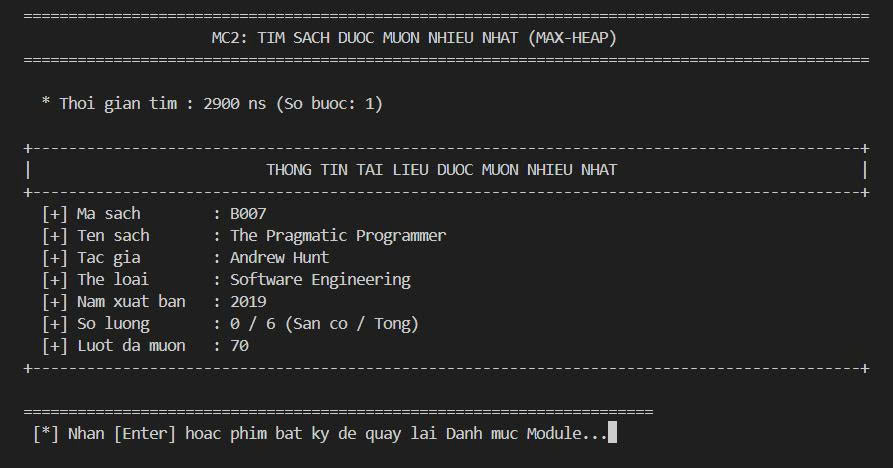
\includegraphics[width=0.78\linewidth]{mc2_normal_view.jpg}
    \caption{Kết quả trích xuất sách được mượn nhiều nhất bằng Max-Heap (Normal Mode)}
    \label{fig:mc2_normal}
\end{figure}

Giao diện thực thi tại Hình \ref{fig:mc2_normal} ghi nhận cuốn sách có lượt mượn cao nhất là \texttt{B007} (\textit{The Pragmatic Programmer}, tác giả \textit{Andrew Hunt}, thể loại \textit{Software Engineering}, số lượt mượn đạt $70$). Thao tác này hoàn tất chỉ trong đúng $1$ bước truy xuất mảng tại chỉ số gốc, thể hiện ưu thế vượt trội của cấu trúc đống được tổ chức sẵn trong bộ nhớ.

Tại chế độ Benchmark Mode (Hình \ref{fig:mc2_benchmark}), hệ thống thực hiện đo đạc song song giữa phương pháp quét tuyến tính tìm cực đại (Linear Max Scan) và cấu trúc Max-Heap.

\begin{figure}[H]
    \centering
    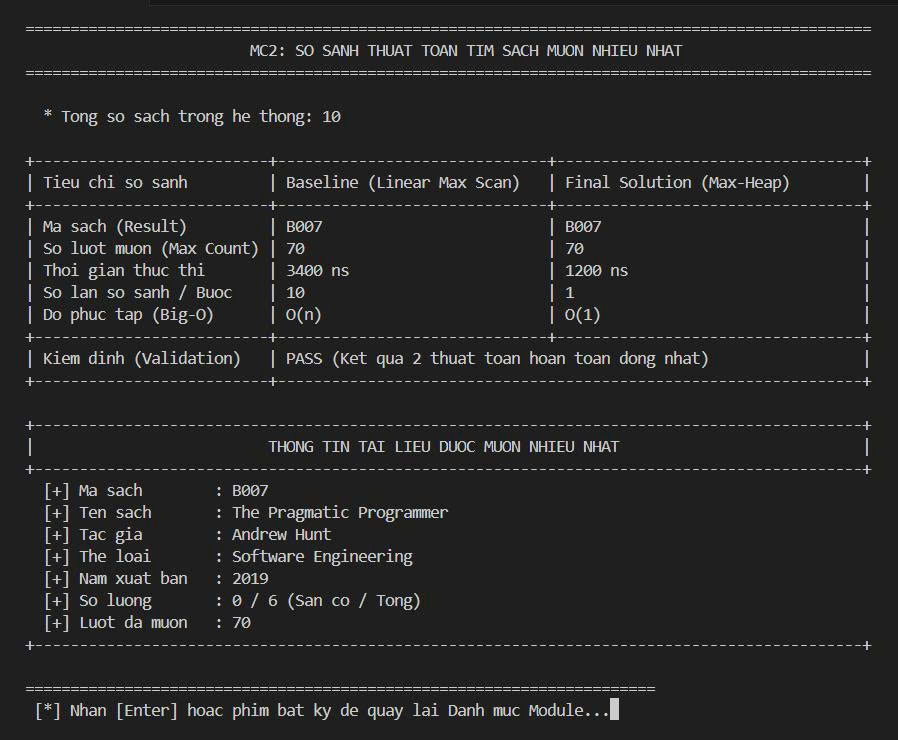
\includegraphics[width=0.76\linewidth]{mc2_benchmark_max.jpg}
    \caption{Đối sánh thực nghiệm giữa Linear Max Scan và Max-Heap trong bài toán tìm cực đại}
    \label{fig:mc2_benchmark}
\end{figure}

Kết quả đối chứng trong Hình \ref{fig:mc2_benchmark} khẳng định cả hai giải pháp đều xác định chính xác cùng một tài liệu cực đại (\texttt{B007} với $70$ lượt mượn), đạt trạng thái kiểm định \texttt{PASS}. Về mặt cơ chế xử lý, trong khi Linear Max Scan phải duyệt qua toàn bộ $10$ phần tử ($10$ phép so sánh) để tìm phần tử lớn nhất, Max-Heap chỉ cần $1$ bước truy xuất phần tử tại đỉnh đống với độ phức tạp lý thuyết $O(1)$. Ở lần chạy mẫu minh họa này, thời gian ghi nhận của Max-Heap là $1.200\text{ ns}$ so với $3.400\text{ ns}$ của Linear Max Scan, phản ánh trực quan sự khác biệt giữa việc tính toán lại từ đầu và việc duy trì cấu trúc dữ liệu có sẵn.

Mở rộng kịch bản kiểm thử lên tập dữ liệu quy mô $500.000$ cuốn sách trên DSA Performance Dashboard (Web), hệ thống tiến hành đối sánh hiệu năng thao tác truy xuất một cuốn sách có số lượt mượn cao nhất (Top 1) như thể hiện trong Hình \ref{fig:web-mc2-top1}.

\begin{figure}[H]
    \centering
    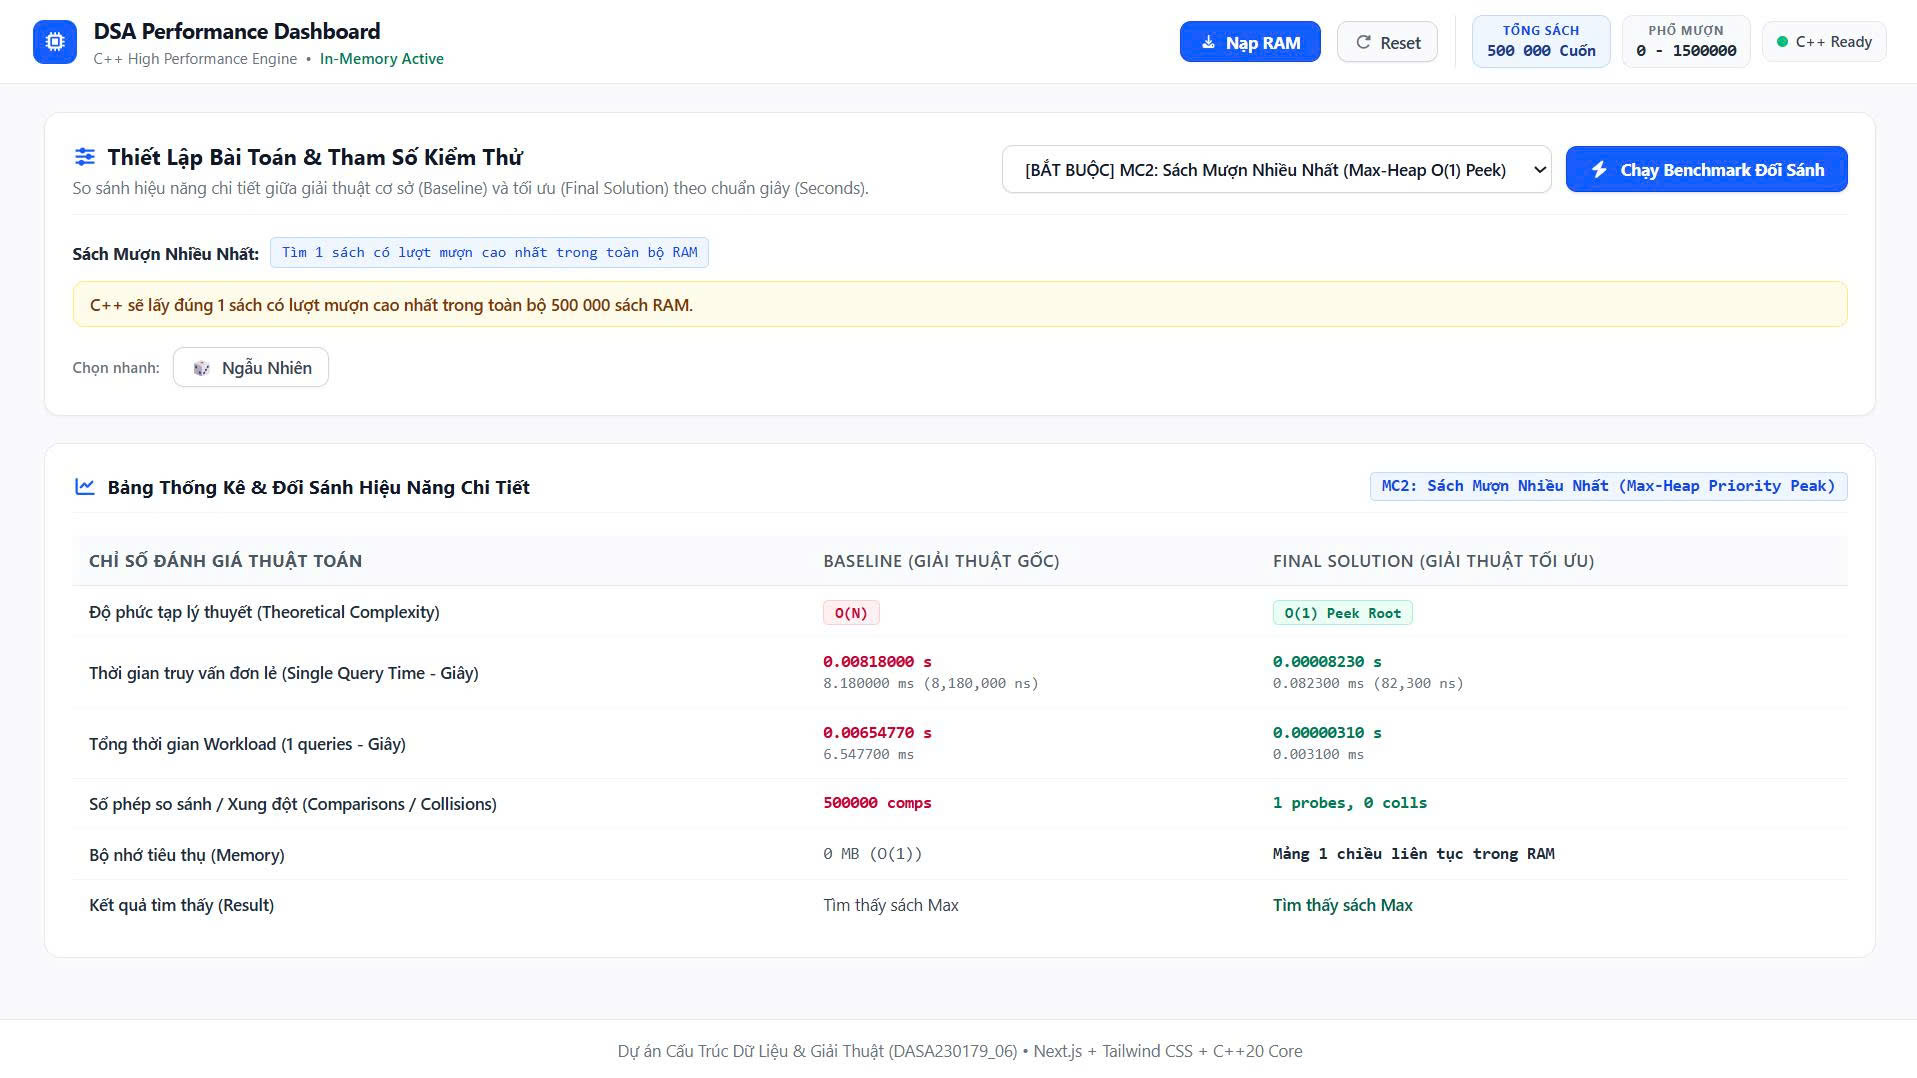
\includegraphics[width=0.88\linewidth]{mc2_benchmark_top1_peek.jpg}
    \caption{So sánh hiệu năng tìm sách có lượt mượn cao nhất (MC2)}
    \label{fig:web-mc2-top1}
\end{figure}

Trong lần chạy đo đạc tại Hình \ref{fig:web-mc2-top1}, Baseline (Linear Max Scan) phải quét qua toàn bộ $500.000$ bản ghi, thực hiện $500.000$ phép so sánh số lượt mượn để tìm giá trị lớn nhất, tiêu tốn $8.18\text{ ms}$ cho một truy vấn đơn. Trong khi đó, cấu trúc Max-Heap trích xuất trực tiếp phần tử cực đại nằm tại đỉnh đống với đúng $1$ probe, $0$ va chạm, ghi nhận thời gian phản hồi chỉ $0.082\text{ ms}$. Cả hai giải pháp đều xác định chính xác cùng một đầu sách có số lượt mượn lớn nhất (PASS).

Tổng hợp đánh giá Module MC2: Module MC2 tập trung giải quyết bài toán truy xuất đầu sách có số lượt mượn cao nhất (Top 1). Thuật toán Baseline buộc phải duyệt lại toàn bộ kho dữ liệu sau mỗi lần truy vấn ($O(N)$), khiến chi phí tăng tuyến tính khi số lượng sách mở rộng. Ngược lại, Cây đống cực đại Max-Heap duy trì trật tự một phần thông qua quan hệ nút cha -- con, cho phép thao tác xem phần tử dẫn đầu (\texttt{peek}) đạt thời gian hằng số $O(1)$. Đánh đổi cho tốc độ tức thời này là chi phí bộ nhớ phụ khoảng $4.00\text{ MB}$ cho mảng đống liên tục cùng chi phí cập nhật $O(\log N)$ khi số lượt mượn của một cuốn sách thay đổi.

\subsection*{2.4. Hiện thực và phân tích chi tiết Module RQ1: Lọc Sách Theo Thể Loại}
\addcontentsline{toc}{subsection}{2.4. Hiện thực và phân tích chi tiết Module RQ1: Lọc Sách Theo Thể Loại}

\subsubsection*{2.4.1. Thuật toán Baseline: Quét Tuyến tính Lọc Thể Loại $O(N)$}
\addcontentsline{toc}{subsubsection}{2.4.1. Thuật toán Baseline: Quét Tuyến tính Lọc Thể Loại O(N)}

Thuật toán Baseline cho yêu cầu lọc sách theo thể loại thực hiện duyệt qua toàn bộ mảng dữ liệu sách, so sánh chuỗi thể loại của từng cuốn với tên thể loại người dùng yêu cầu. Mỗi khi gặp một cuốn sách phù hợp, bản ghi đó sẽ được sao chép vào danh sách kết quả trả về.

Phương pháp này luôn phải kiểm tra tất cả các phần tử trong kho sách, bất kể thể loại được chọn có chứa nhiều sách hay chỉ có một vài cuốn. Chi phí thời gian luôn phụ thuộc vào tổng quy mô toàn bộ thư viện, làm giảm đáng kể tốc độ phản hồi khi số lượng đầu sách lớn.

\subsubsection*{2.4.2. Cấu trúc Tối ưu: Phân Cụm Bảng Băm Danh Mục (Category Hash Table)}
\addcontentsline{toc}{subsubsection}{2.4.2. Cấu trúc Tối ưu: Phân Cụm Bảng Băm Danh Mục (Category Hash Table)}

Giải pháp tối ưu xây dựng một Bảng băm đa trị (Category Hash Table), trong đó khóa băm là tên thể loại và giá trị lưu trữ là một danh sách chứa toàn bộ các cuốn sách thuộc thể loại đó.

\begin{figure}[H]
    \centering
    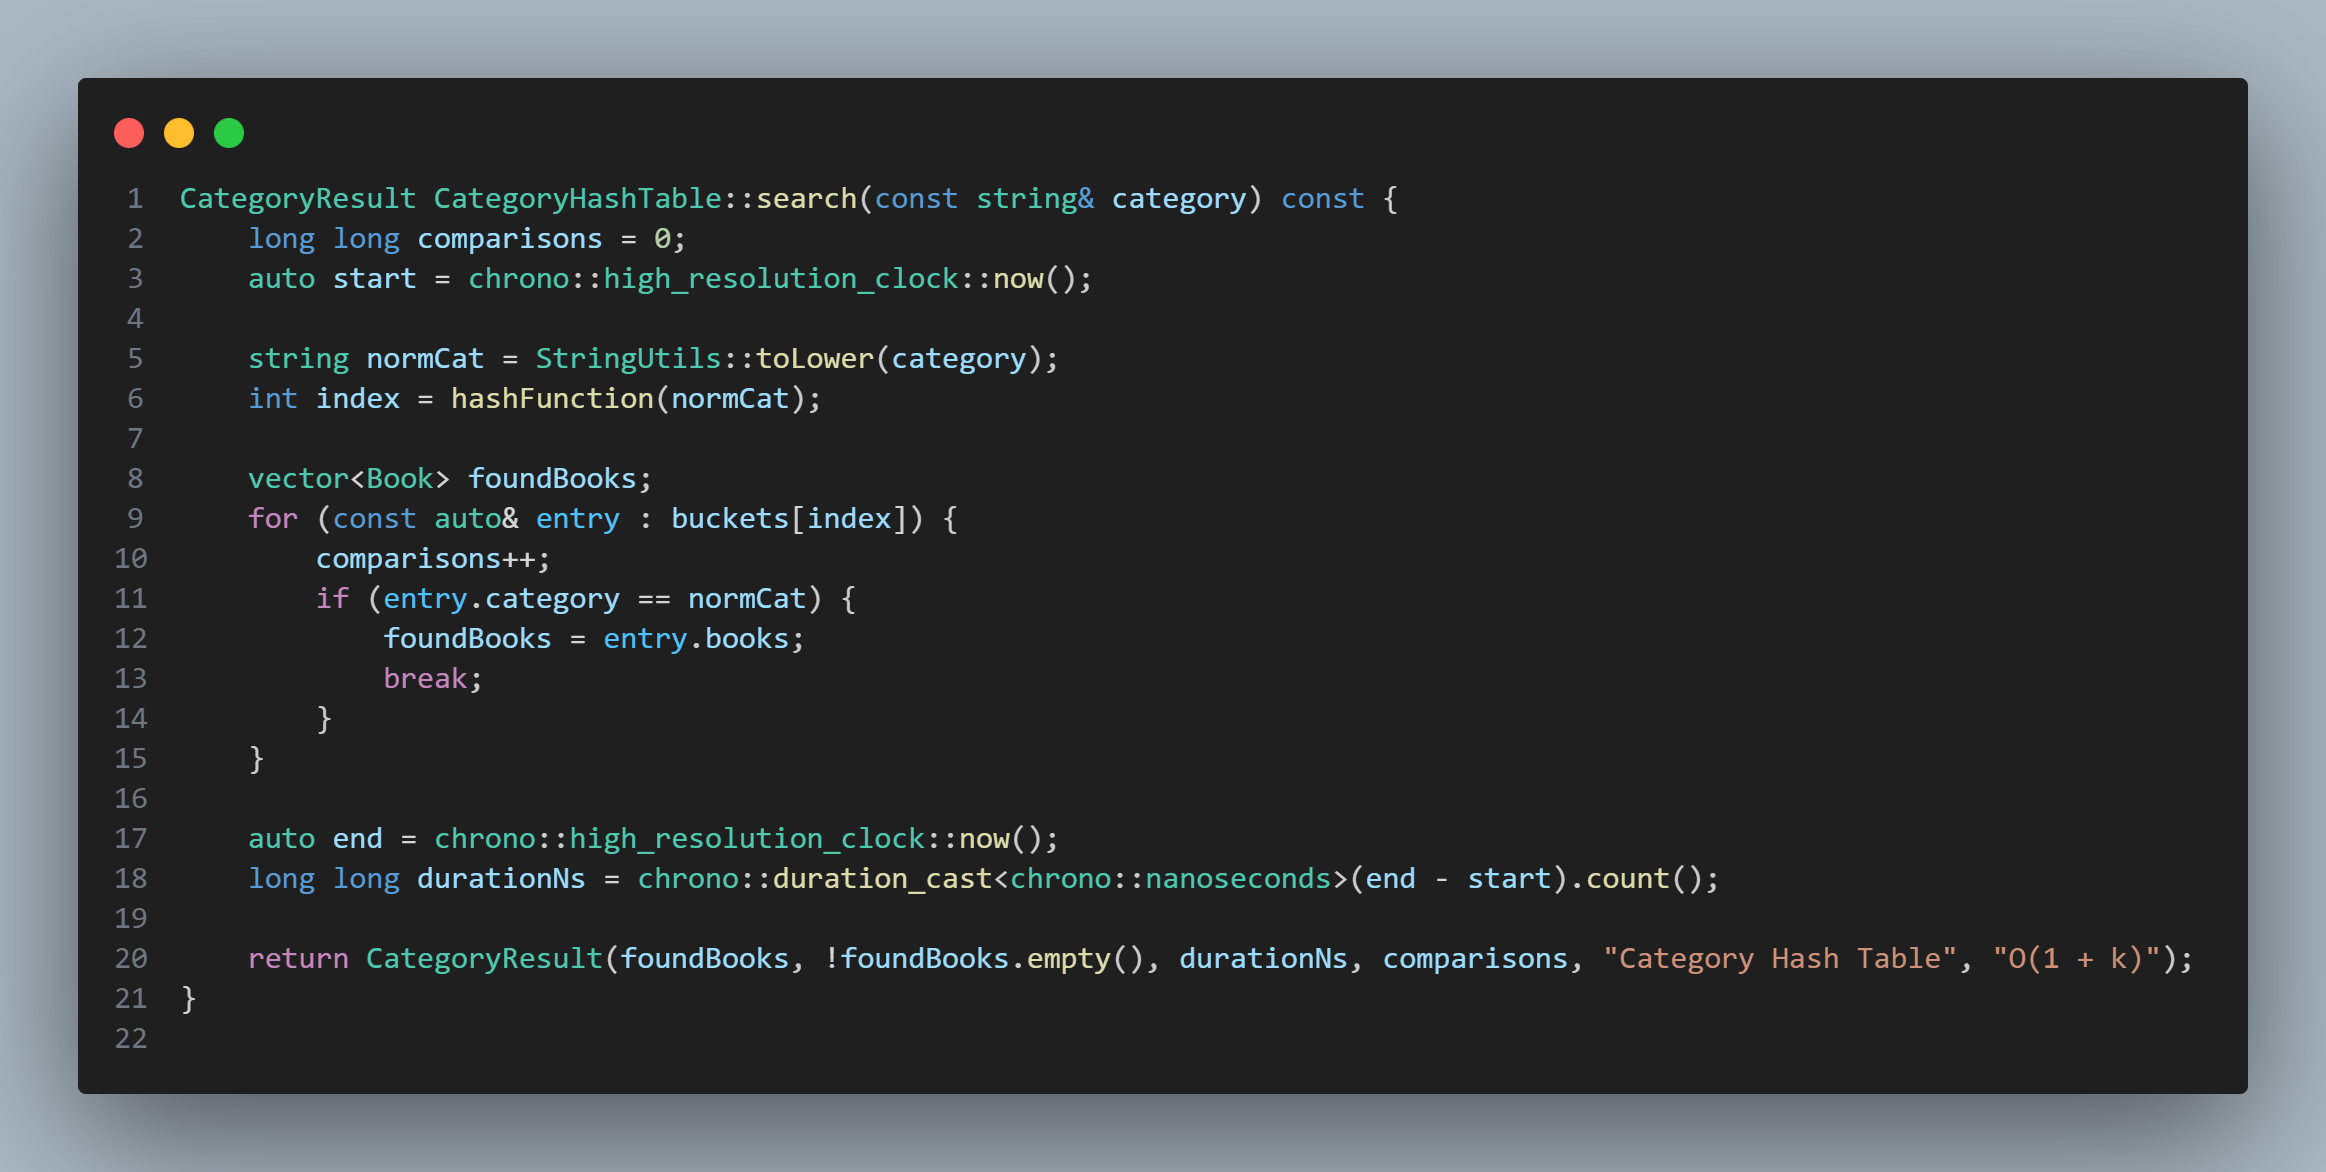
\includegraphics[width=0.88\linewidth]{code_rq1_category_hash_search.png}
    \caption{Hiện thực hàm tra cứu danh mục thể loại trong Bảng băm gom cụm}
    \label{fig:code_rq1_search}
\end{figure}

Hình \ref{fig:code_rq1_search} minh họa hàm tìm kiếm danh mục thể loại. Khi xây dựng cấu trúc, mỗi cuốn sách được phân cụm sẵn vào danh mục tương ứng. Khi tra cứu, hệ thống băm tên thể loại để định vị trực tiếp ô chứa danh mục trong thời gian hằng số, sau đó trả về danh sách các sách đã được gom nhóm từ trước.

\subsubsection*{2.4.3. Truy xuất Danh mục $O(1+K)$ \& Sơ đồ Tuần tự}
\addcontentsline{toc}{subsubsection}{2.4.3. Truy xuất Danh mục O(1+K) \& Sơ đồ Tuần tự}

Nhờ cơ chế gom cụm sẵn, thời gian thực thi của thao tác lọc thể loại chỉ bao gồm thời gian hằng số để định vị nhóm cộng với thời gian tỉ lệ thuận theo số lượng sách thực tế của thể loại đó, hoàn toàn độc lập với tổng số lượng sách của toàn bộ thư viện.

\begin{figure}[H]
    \centering
    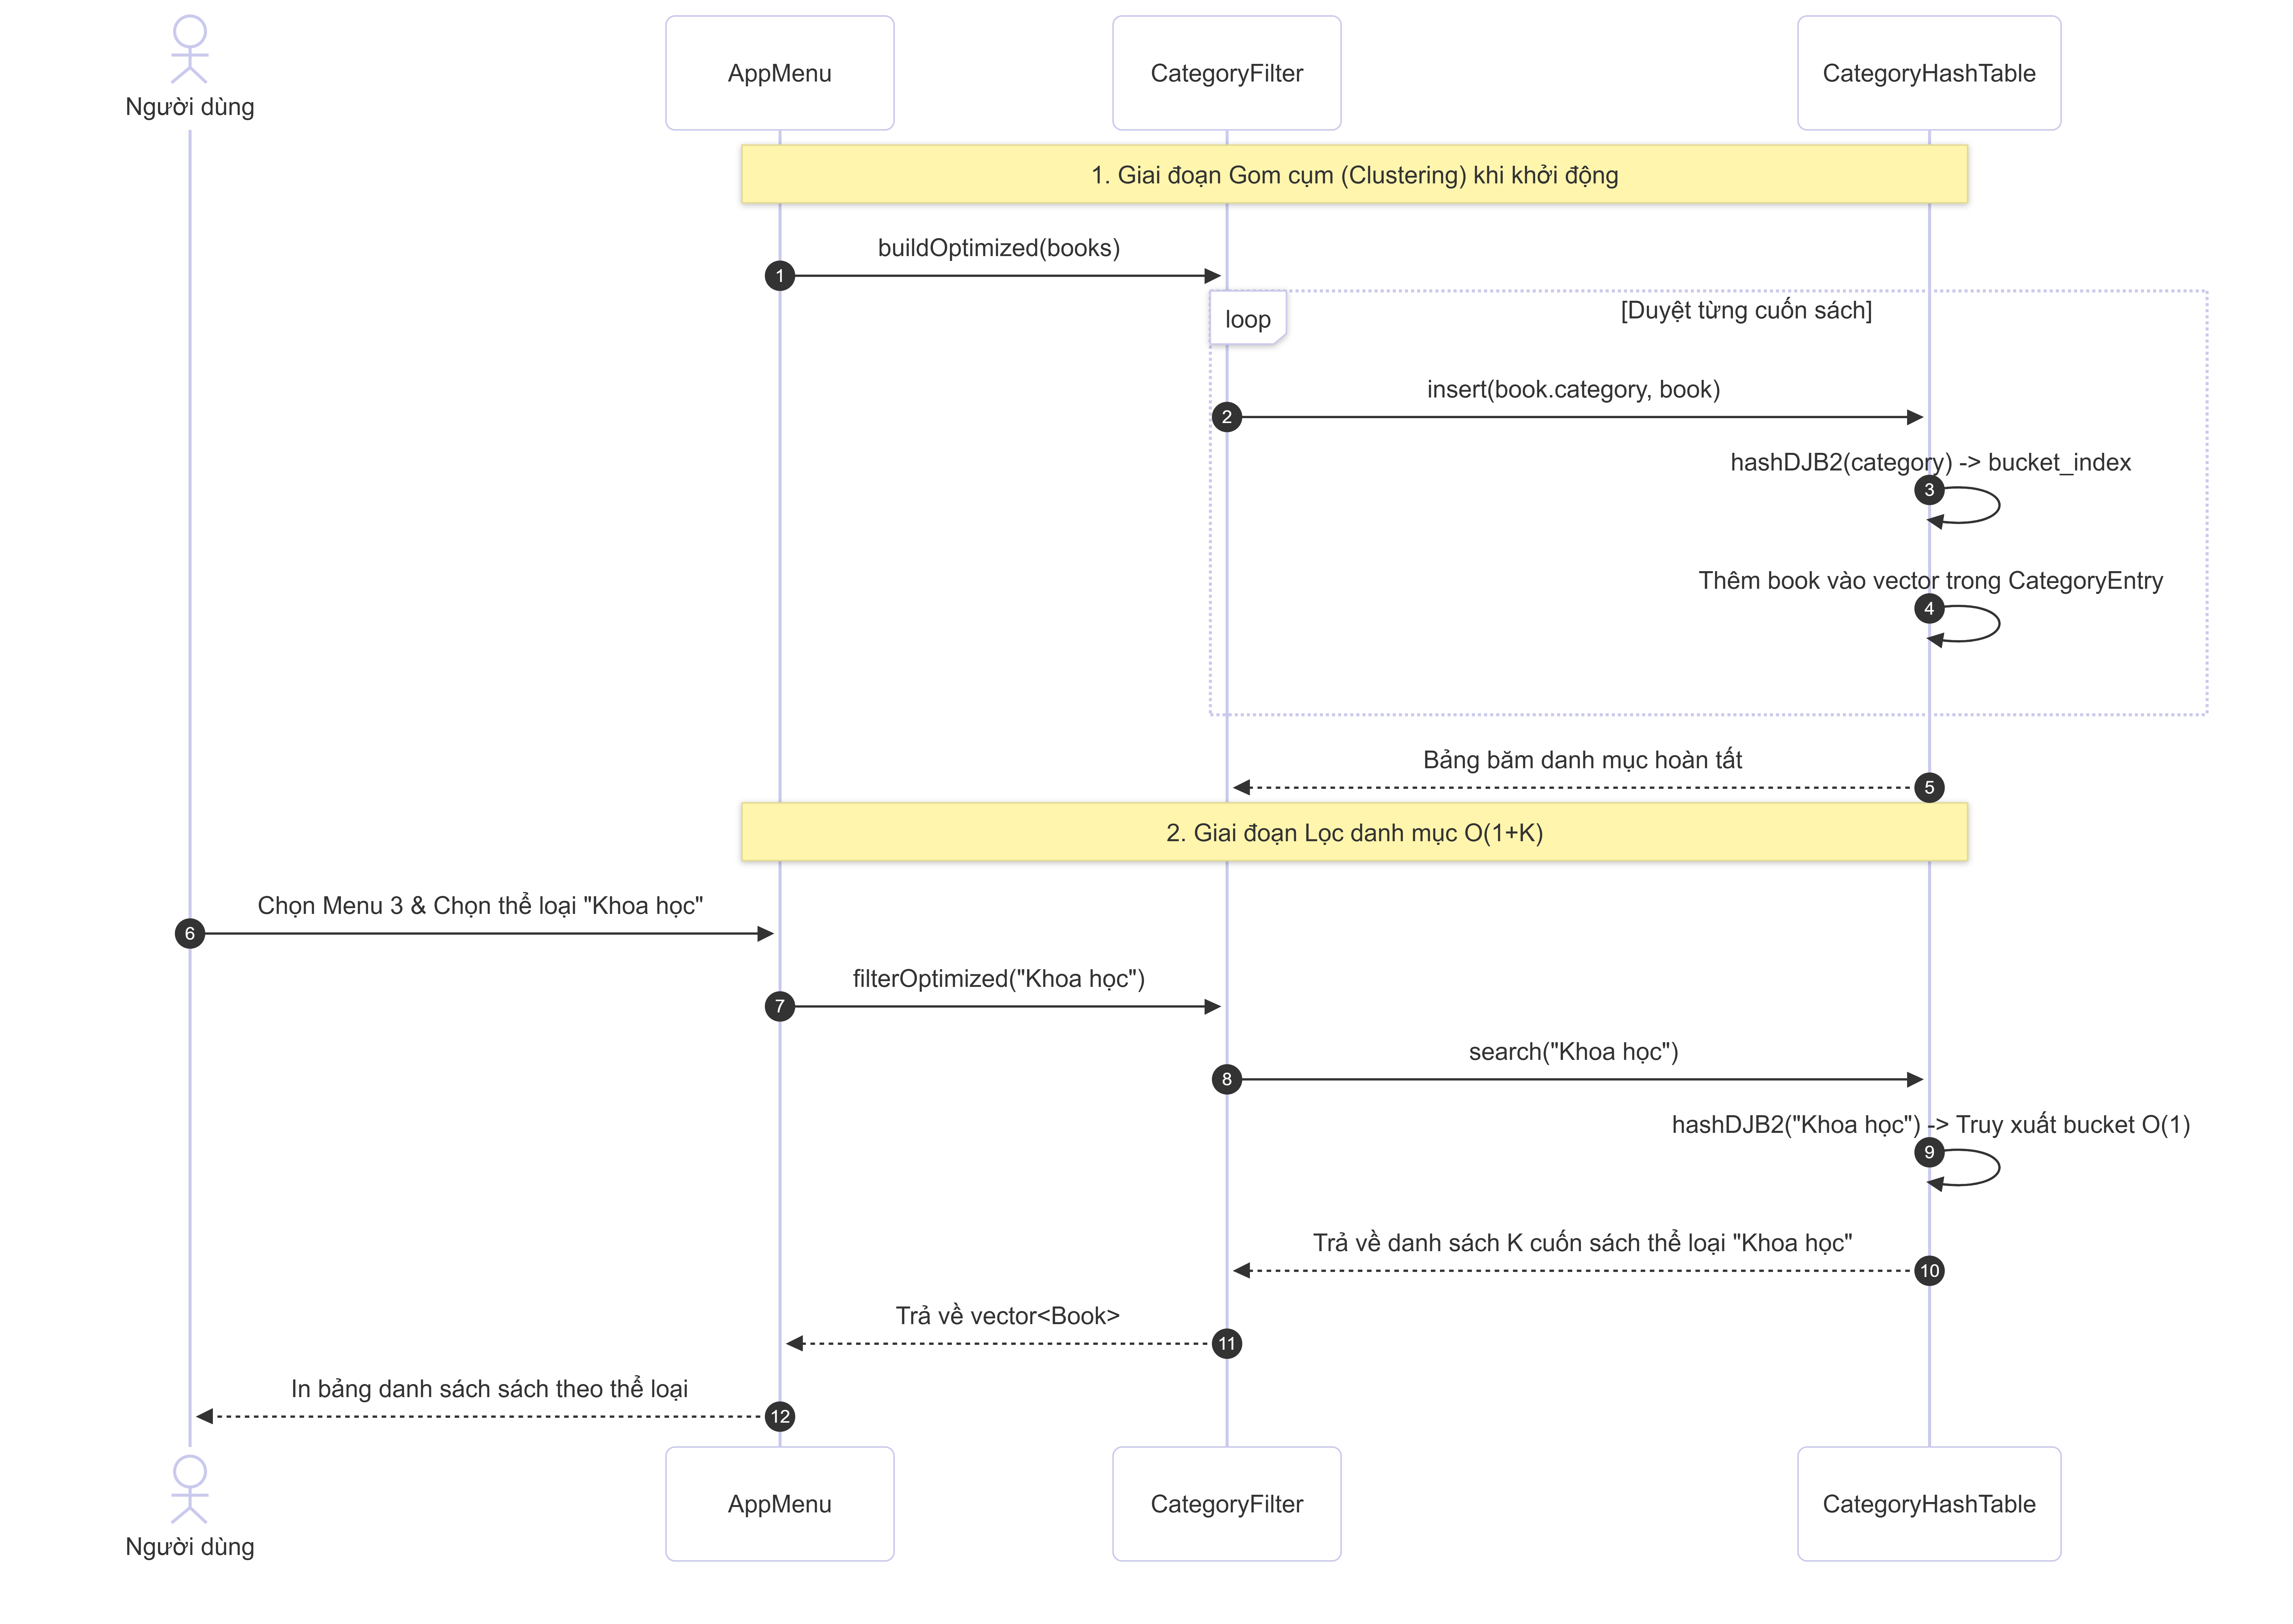
\includegraphics[width=0.85\linewidth]{seq_rq1_category_filter.png}
    \caption{Sơ đồ tuần tự thể hiện luồng lọc sách theo thể loại (RQ1)}
    \label{fig:seq_rq1}
\end{figure}

Sơ đồ tuần tự tại Hình \ref{fig:seq_rq1} thể hiện luồng đối sánh giữa việc quét tuyến tính toàn bộ kho sách và việc truy xuất trực tiếp từ Bảng băm danh mục, chứng minh tính hiệu quả rõ rệt của giải pháp gom cụm dữ liệu.

\subsubsection*{2.4.4. Thực nghiệm kiểm chứng trên Giao diện dòng lệnh (CLI Validation)}
\addcontentsline{toc}{subsubsection}{2.4.4. Thực nghiệm kiểm chứng trên Giao diện dòng lệnh (CLI Validation)}

Cần nhấn mạnh rằng Module RQ1 là bài toán truy vấn và trả về toàn bộ tất cả các cuốn sách thuộc một thể loại xác định, hoàn toàn không phải là bài toán xếp hạng Top-$K$ hay chọn lọc theo số lượng giới hạn. Để kiểm chứng tính đúng đắn và tốc độ truy xuất, nhóm đã thử nghiệm Module RQ1 trên giao diện CLI ở cả hai chế độ vận hành.

Trong chế độ Normal Mode, người dùng thực hiện tra cứu thể loại \texttt{Computer Science}. Hệ thống sử dụng Bảng băm danh mục (Category Hash Table) để định vị nhóm và kết xuất toàn bộ danh sách sách thuộc thể loại này (Hình \ref{fig:rq1_normal}).

\begin{figure}[H]
    \centering
    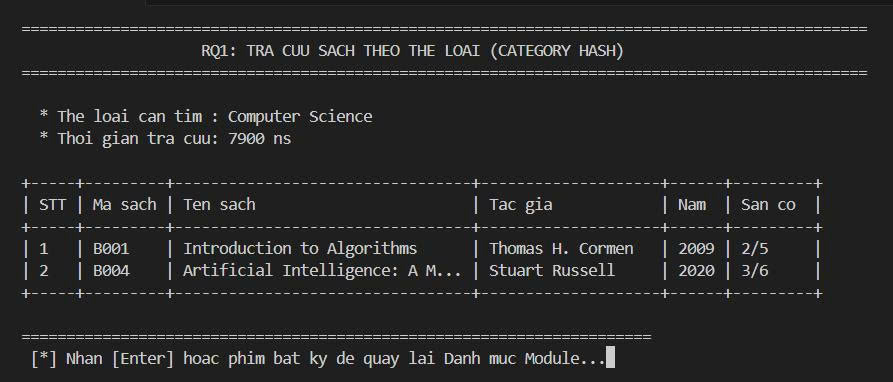
\includegraphics[width=0.78\linewidth]{rq1_normal_view.jpg}
    \caption{Kết quả tra cứu toàn bộ sách thuộc thể loại Computer Science bằng Category Hash Table}
    \label{fig:rq1_normal}
\end{figure}

Kết quả trên Hình \ref{fig:rq1_normal} hiển thị đầy đủ danh sách gồm 2 cuốn sách thuộc thể loại \textit{Computer Science} có trong tập dữ liệu mẫu: \texttt{B001} (\textit{Introduction to Algorithms}) và \texttt{B004} (\textit{Artificial Intelligence: A Modern Approach}). Nhờ việc phân cụm sẵn các con trỏ sách vào danh sách liên kết tại ô băm tương ứng, hệ thống chỉ cần duyệt qua đúng số lượng phần tử thực tế của nhóm đó mà không phải rà soát qua các thể loại khác.

Tiếp tục đánh giá ở chế độ Benchmark Mode, Hình \ref{fig:rq1_found} ghi nhận trường hợp tra cứu thể loại \texttt{Database} trên tập dữ liệu thử nghiệm 10 cuốn sách.

\begin{figure}[H]
    \centering
    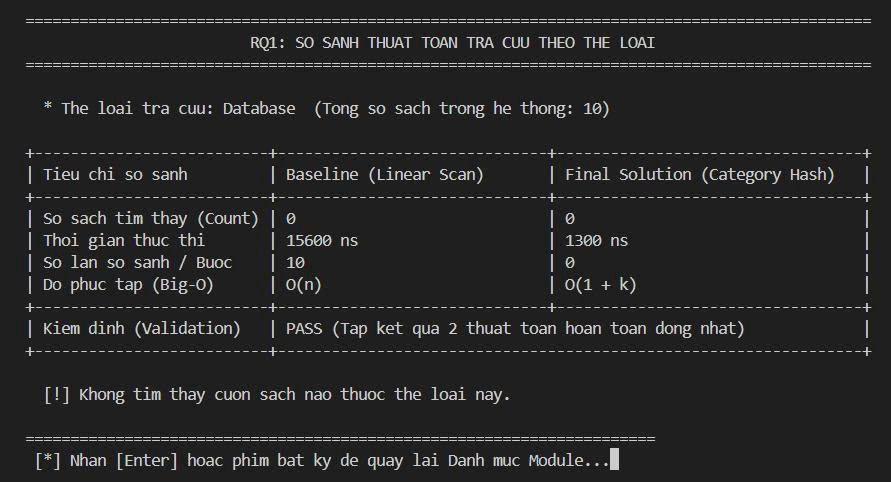
\includegraphics[width=0.78\linewidth]{rq1_benchmark_found.jpg}
    \caption{Đối sánh giữa Linear Scan và Category Hash khi tra cứu thể loại mẫu trên hệ thống}
    \label{fig:rq1_found}
\end{figure}

Hình \ref{fig:rq1_found} phản ánh trường hợp thể loại \texttt{Database} trong tập dữ liệu mẫu ban đầu chưa chứa bản ghi sách nào (Count = $0$). Cả hai phương pháp đều đưa ra kết luận đồng nhất ($0$ sách tìm thấy) và đạt trạng thái \texttt{PASS}. Về mặt số bước thực hiện, Linear Scan vẫn phải duyệt qua toàn bộ $10$ cuốn sách trong kho để kiểm tra từng chuỗi thể loại, trong khi Category Hash định vị ô băm rỗng trong thời gian $O(1)$ với $0$ phép so sánh chuỗi lặp lại.

Đối với trường hợp kiểm thử thể loại hoàn toàn không tồn tại trong danh mục hệ thống (ví dụ thể loại \texttt{Cooking}), kết quả đối sánh được thể hiện trong Hình \ref{fig:rq1_notfound}.

\begin{figure}[H]
    \centering
    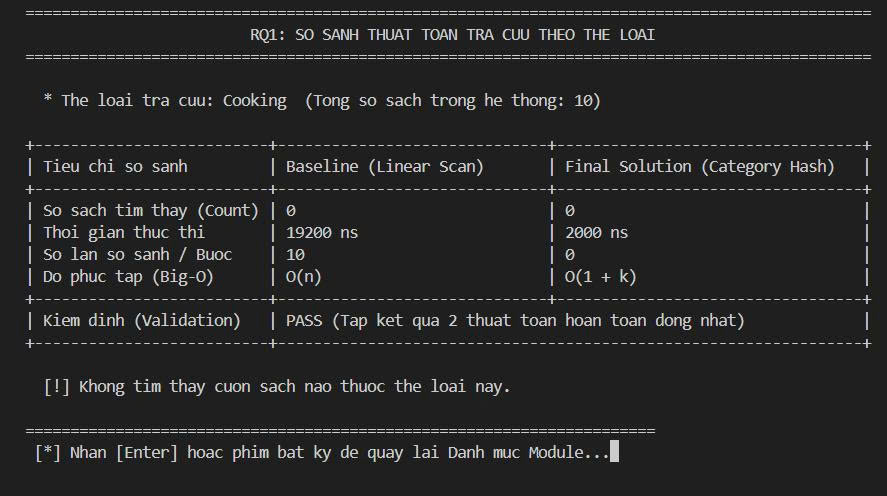
\includegraphics[width=0.78\linewidth]{rq1_benchmark_notfound.jpg}
    \caption{Đối sánh thực nghiệm giữa Linear Scan và Category Hash khi thể loại không tồn tại}
    \label{fig:rq1_notfound}
\end{figure}

Tương tự như trường hợp trên, Hình \ref{fig:rq1_notfound} cho thấy Linear Scan tiêu tốn $10$ lần so sánh chuỗi trên toàn mảng, trong khi Category Hash Table nhận biết ngay khóa băm chưa từng được khởi tạo và kết thúc trong $0$ bước so sánh chuỗi, khẳng định tính ưu việt của mô hình phân cụm chỉ mục trước.

Tiếp tục đánh giá Module RQ1 trên quy mô $500.000$ cuốn sách tại DSA Performance Dashboard (Web), hệ thống tiến hành kiểm chứng hai kịch bản: thể loại có số lượng sách lớn và thể loại không tồn tại.

\begin{figure}[H]
    \centering
    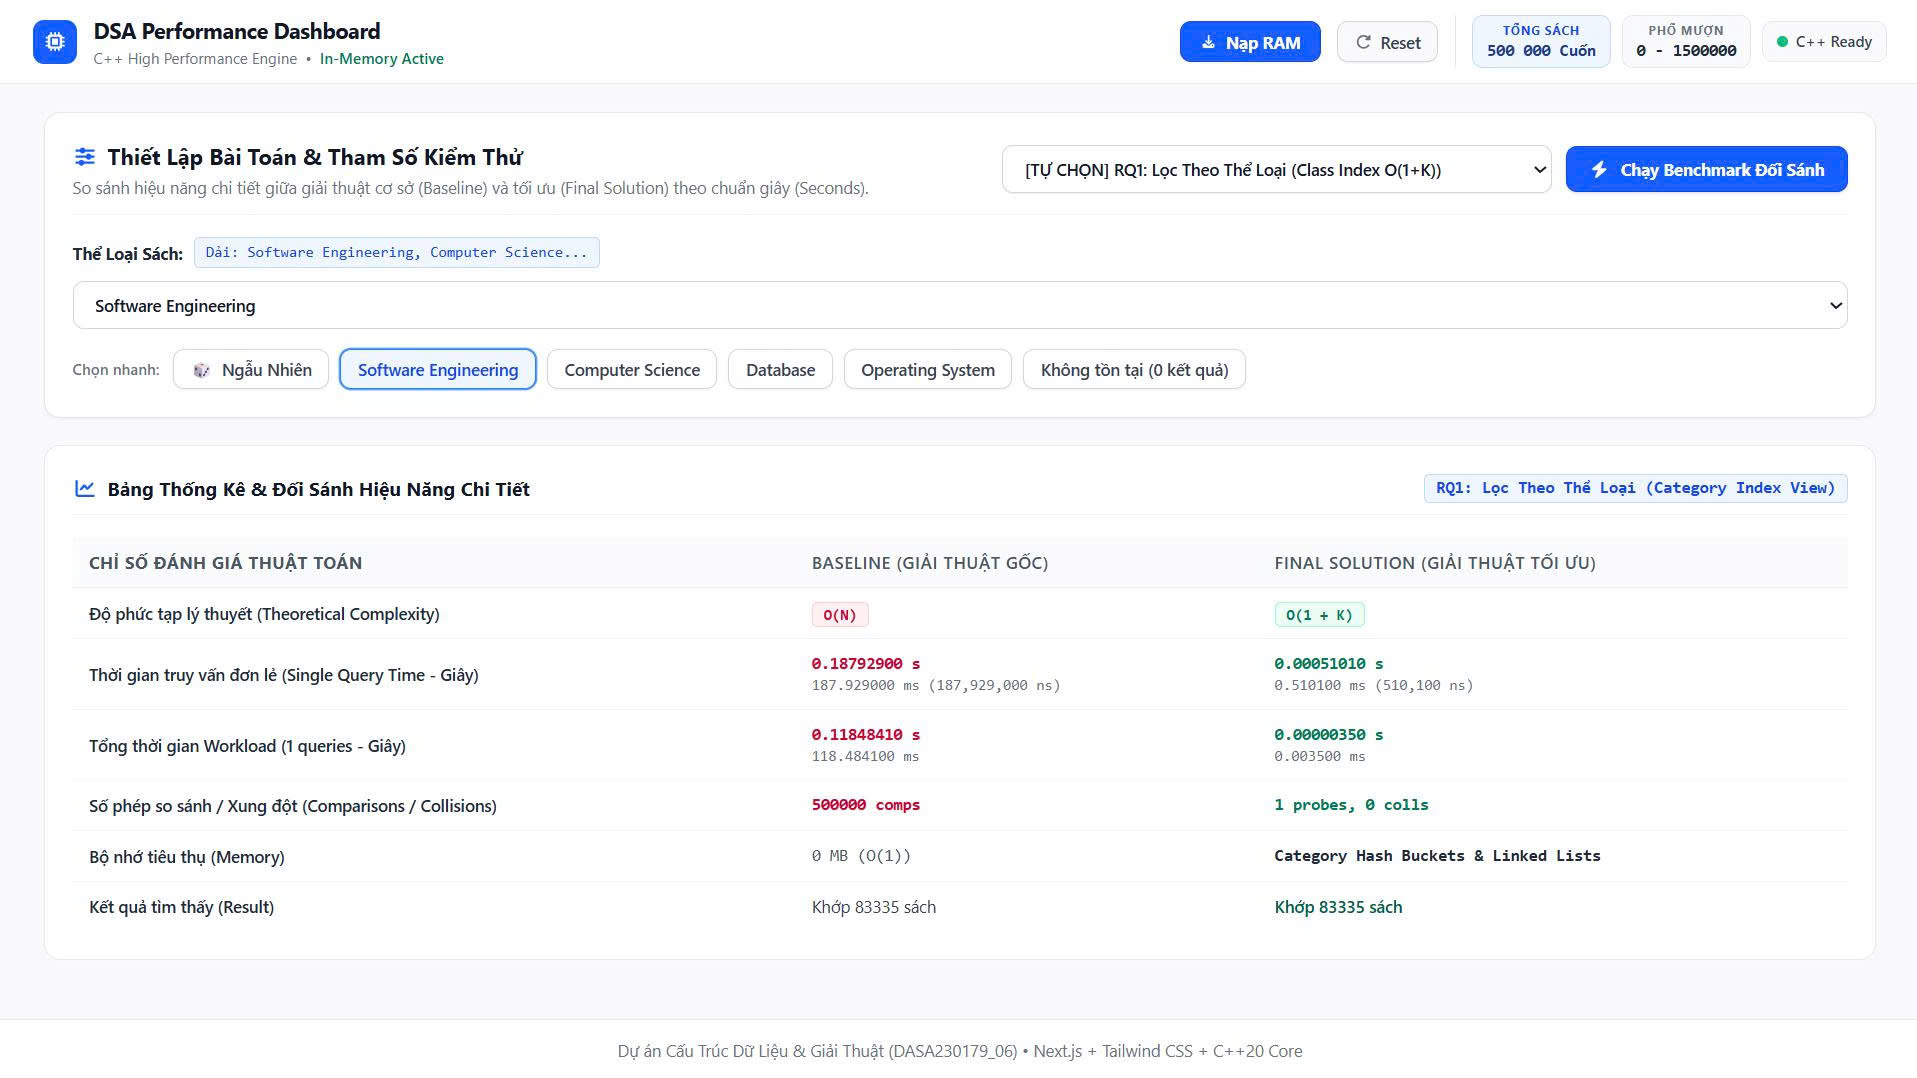
\includegraphics[width=0.88\linewidth]{rq1_benchmark_category_found.jpg}
    \caption{Benchmark RQ1 với thể loại tồn tại (Software Engineering)}
    \label{fig:web-rq1-found}
\end{figure}

Ở kịch bản thể loại tồn tại trong cơ sở dữ liệu (\texttt{Software Engineering}) tại Hình \ref{fig:web-rq1-found}, hệ thống ghi nhận có tới $83.335$ cuốn sách thuộc thể loại này trong tổng số $500.000$ sách. Thuật toán Linear Scan phải quét toàn bộ $500.000$ bản ghi, tiêu tốn $187.9\text{ ms}$ cho một truy vấn đơn. Trong khi đó, Category Hash Table định vị trực tiếp nhóm danh mục với $1$ probe, $0$ va chạm và trích xuất danh sách liên kết chứa $83.335$ cuốn sách trong $0.510\text{ ms}$. Cả hai giải pháp đều trả về chính xác $83.335$ cuốn sách khớp, đạt trạng thái kiểm định \texttt{PASS}. Cần lưu ý rằng việc duyệt và trả về tập kết quả lớn ($K = 83.335$) vẫn đòi hỏi chi phí tỉ lệ theo $K$, song giải pháp tối ưu đã loại bỏ hoàn toàn việc phải rà soát qua $416.665$ cuốn sách không liên quan.

\begin{figure}[H]
    \centering
    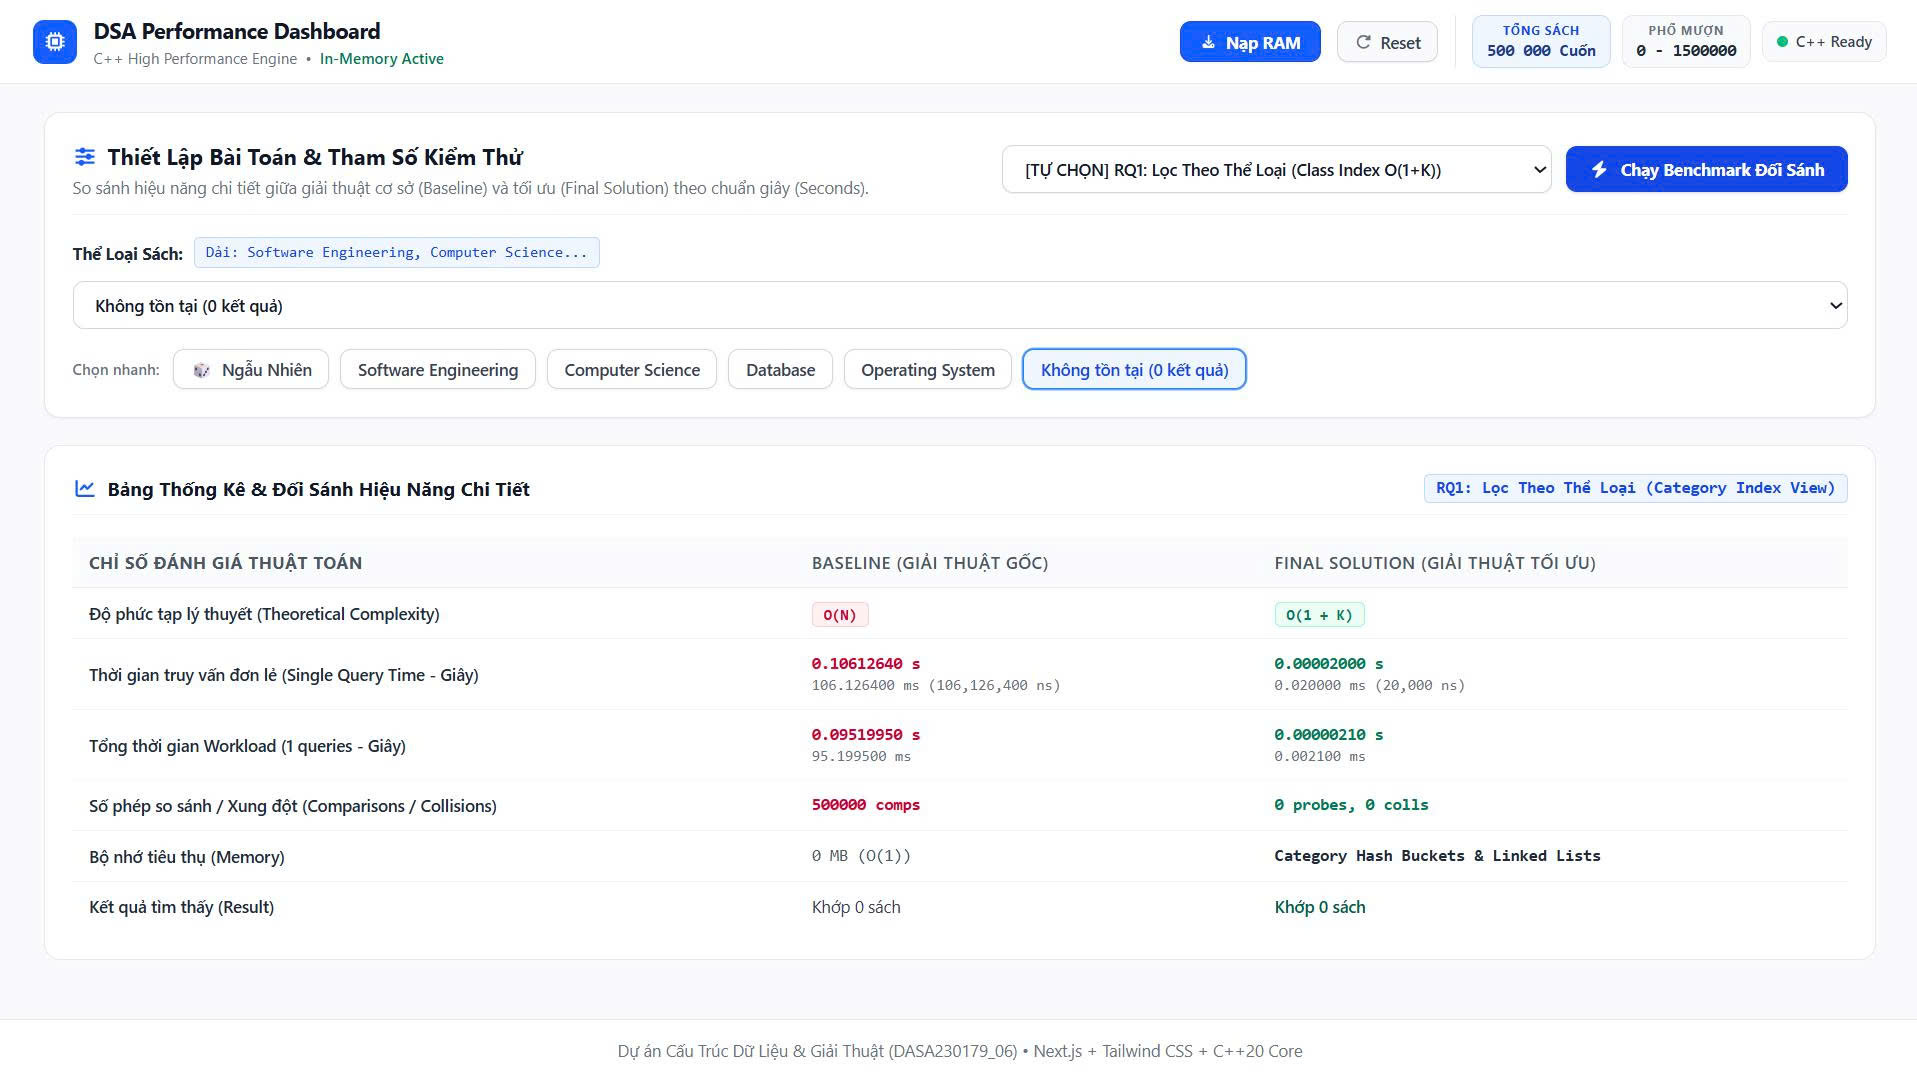
\includegraphics[width=0.88\linewidth]{rq1_benchmark_category_not_found.jpg}
    \caption{Benchmark RQ1 với thể loại không tồn tại}
    \label{fig:web-rq1-notfound}
\end{figure}

Đối với trường hợp thể loại hoàn toàn không tồn tại trong tập dữ liệu (Hình \ref{fig:web-rq1-notfound}), Linear Scan vẫn phải duyệt tuần tự qua toàn bộ $500.000$ cuốn sách ($106.1\text{ ms}$) để khẳng định không có kết quả. Ngược lại, Category Hash Table nhận diện ngay ô băm rỗng với $0$ probe ($0.020\text{ ms}$) và kết thúc tức thì, cả hai phương pháp đều trả về $0$ sách (PASS).

Tổng hợp đánh giá Module RQ1: Module RQ1 là bài toán truy vấn và thu thập tất cả các tài liệu thuộc một thể loại xác định (không phải bài toán xếp hạng hay cắt lọc Top-$K$). Kết quả thực nghiệm khẳng định việc tổ chức chỉ mục phân cụm sẵn (Category Hash Index) giúp chi phí tìm kiếm đạt độ phức tạp $O(1 + K)$, với $K$ là số lượng phần tử thuộc nhóm kết quả. Đánh đổi lại, hệ thống cần thêm khoảng $5.09\text{ MB}$ bộ nhớ phụ để lưu trữ mảng bucket băm và danh sách liên kết gom nhóm.

\subsection*{2.5. Hiện thực và phân tích chi tiết Module RQ2: Truy Vết Phiếu Quá Hạn}
\addcontentsline{toc}{subsection}{2.5. Hiện thực và phân tích chi tiết Module RQ2: Truy Vết Phiếu Quá Hạn}

\subsubsection*{2.5.1. Thuật toán Baseline: Quét Tuyến tính Hồ sơ Phiếu mượn $O(N)$}
\addcontentsline{toc}{subsubsection}{2.5.1. Thuật toán Baseline: Quét Tuyến tính Hồ sơ Phiếu mượn O(N)}

Thuật toán Baseline cho bài toán kiểm tra quá hạn thực hiện quét qua toàn bộ danh sách phiếu mượn, phân tích chuỗi ngày hạn trả của từng phiếu và so sánh với ngày kiểm tra hiện tại. Nếu trạng thái phiếu vẫn đang mượn và hạn trả nhỏ hơn ngày kiểm tra, phiếu đó được đưa vào danh sách quá hạn.

Phương pháp này phải rà soát qua toàn bộ các phiếu mượn đã hoàn trả trong quá khứ cũng như các phiếu chưa đến hạn, gây lãng phí lớn tài nguyên CPU khi lịch sử giao dịch của thư viện tích lũy qua nhiều năm học.

\subsubsection*{2.5.2. Cấu trúc Tối ưu: Cây Tự Cân Bằng AVL \& 4 Phép Quay}
\addcontentsline{toc}{subsubsection}{2.5.2. Cấu trúc Tối ưu: Cây Tự Cân Bằng AVL \& 4 Phép Quay}

Giải pháp tối ưu sử dụng Cây tìm kiếm nhị phân tự cân bằng AVL, trong đó mỗi nút trên cây đại diện cho một mốc ngày hẹn trả duy nhất và chứa danh sách các phiếu mượn có cùng hạn trả đó. Khóa so sánh giữa các nút là chuỗi ngày tháng đã được chuẩn hóa.

\begin{figure}[H]
    \centering
    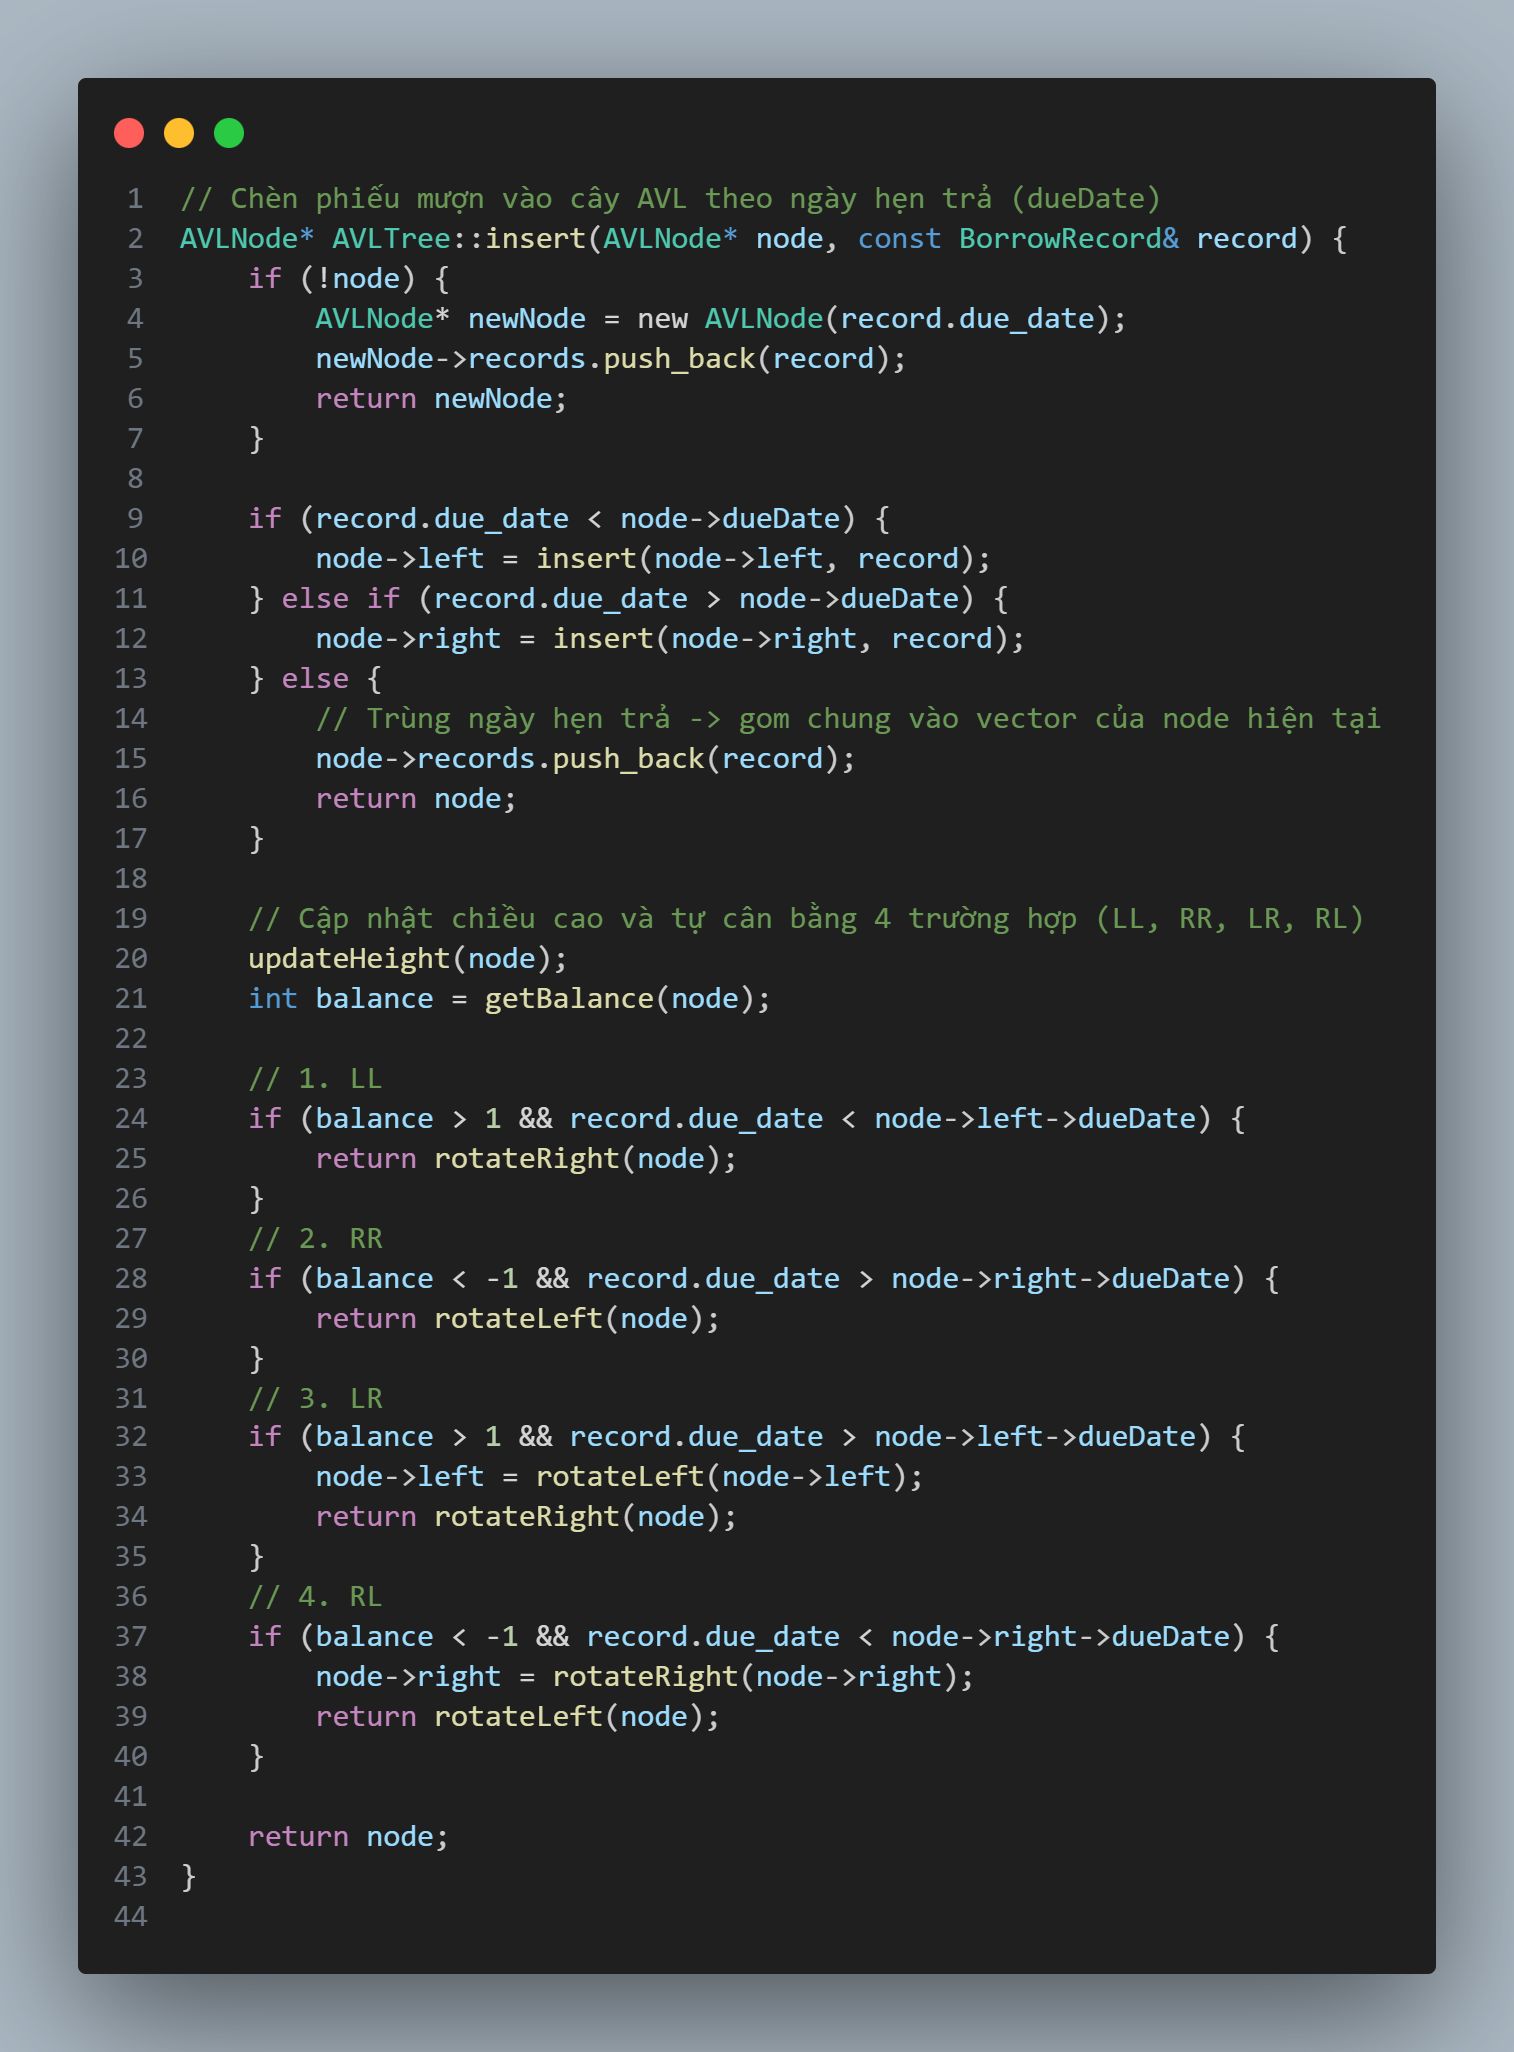
\includegraphics[width=0.85\linewidth]{code_rq2_avl_insert_balance.png}
    \caption{Cài đặt cơ chế kiểm tra hệ số cân bằng và thực hiện phép quay cây AVL}
    \label{fig:code_rq2_avl}
\end{figure}

Để đảm bảo cây không bao giờ bị suy thoái thành danh sách liên kết khi nạp dữ liệu ngày tháng theo thứ tự thời gian, cây AVL liên tục tính toán hệ số cân bằng của từng nút sau mỗi thao tác chèn. Khi phát hiện hệ số cân bằng vượt quá ngưỡng cho phép, cấu trúc tự động kích hoạt một trong bốn phép quay cây tại chỗ như thể hiện ở Hình \ref{fig:code_rq2_avl}, bảo đảm chiều cao của toàn cây luôn bị chặn ở mức logarit theo số lượng mốc ngày.

\subsubsection*{2.5.3. Thuật toán Tỉa Nhánh Khoảng Ngày (Range Query Pruning) $O(\log N + K)$ \& Sơ đồ Tuần tự}
\addcontentsline{toc}{subsubsection}{2.5.3. Thuật toán Tỉa Nhánh Khoảng Ngày (Range Query Pruning) O(log N + K) \& Sơ đồ Tuần tự}

Khi thực hiện truy vấn các phiếu mượn quá hạn trước một ngày kiểm tra, thuật toán duyệt cây áp dụng nguyên lý cắt tỉa nhánh thông minh (Range Query Pruning).

\begin{figure}[H]
    \centering
    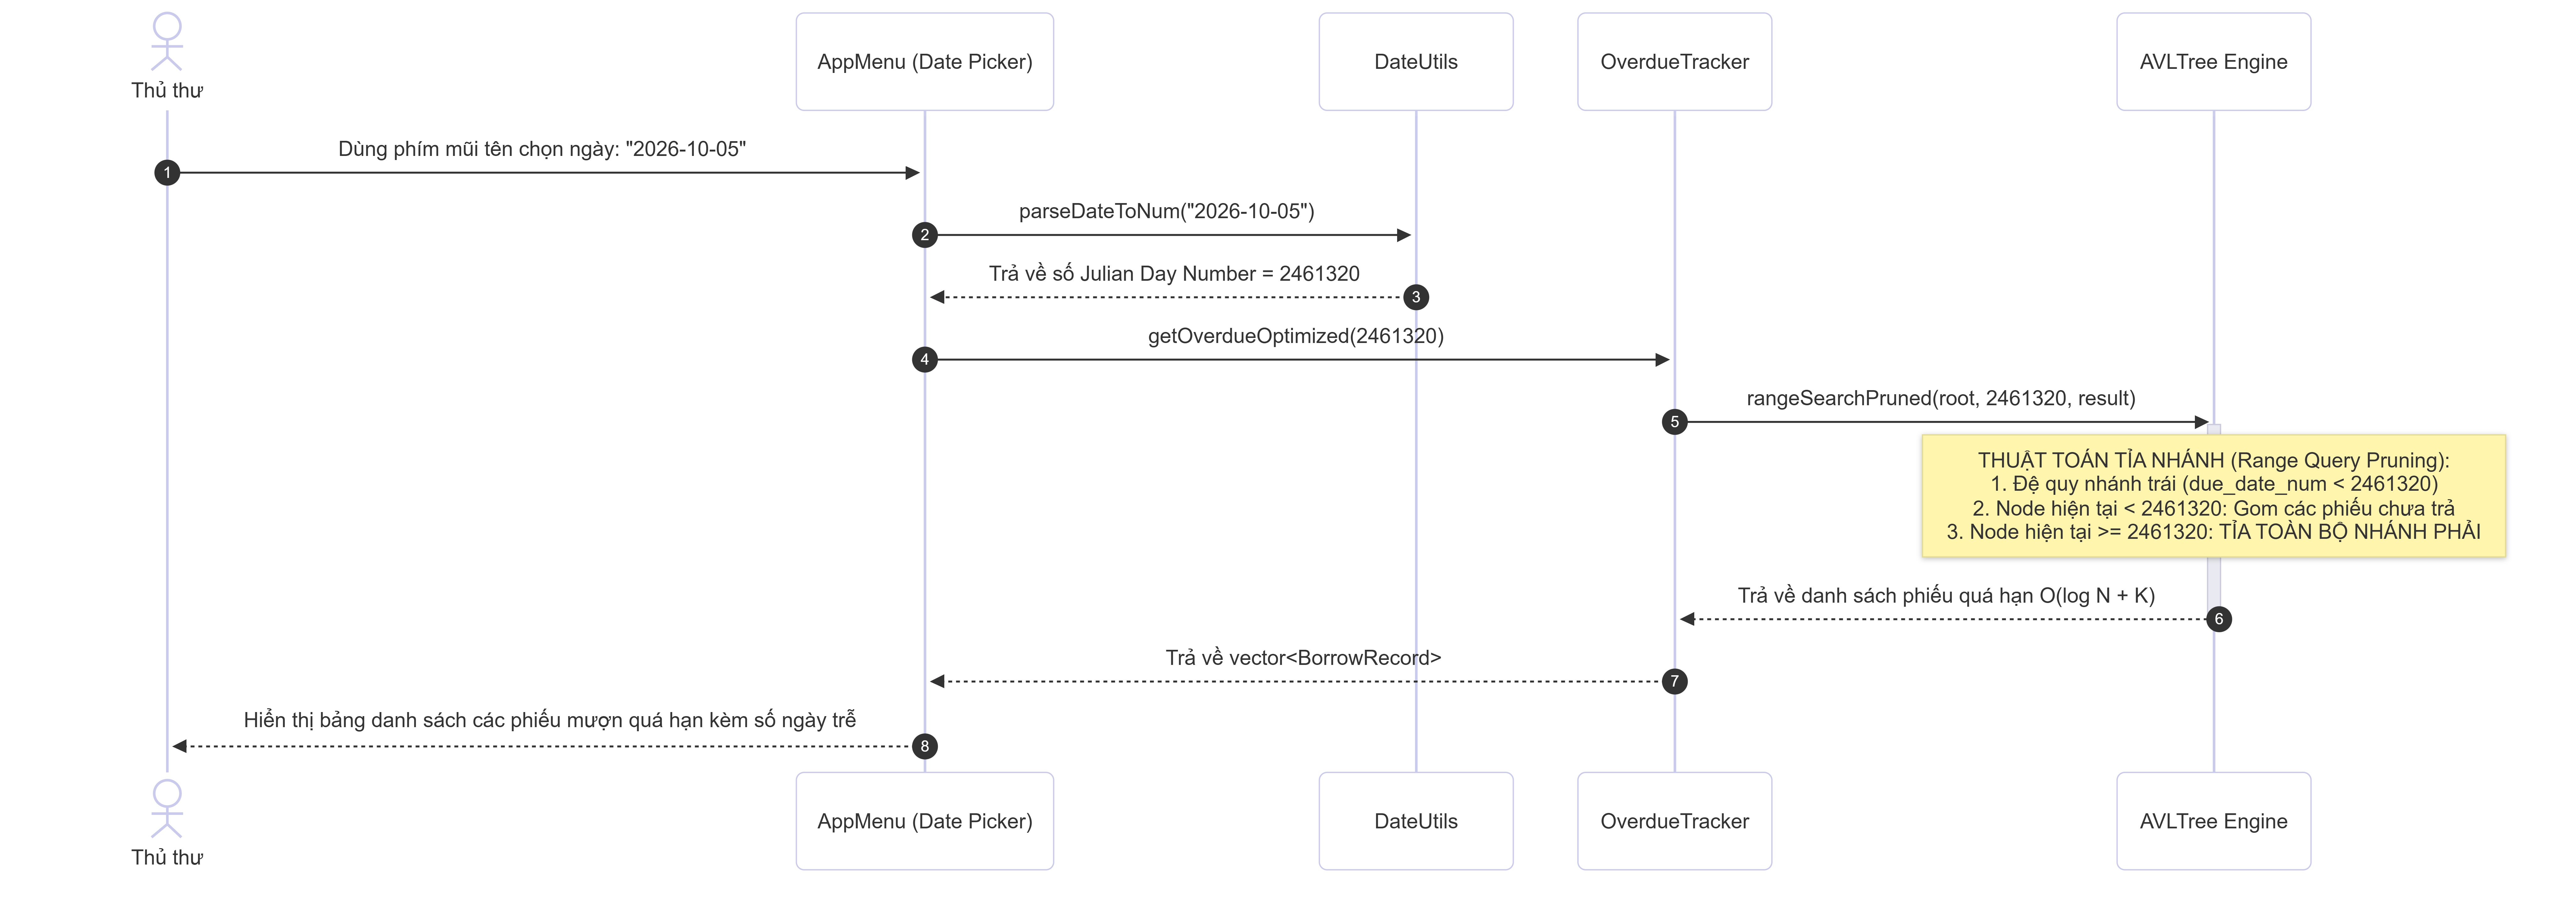
\includegraphics[width=0.82\linewidth]{seq_rq2_overdue_avl_tracker.png}
    \caption{Sơ đồ tuần tự thể hiện luồng truy vết phiếu mượn quá hạn (RQ2)}
    \label{fig:seq_rq2}
\end{figure}

Nếu ngày hẹn trả tại nút hiện tại lớn hơn hoặc bằng ngày kiểm tra, thuật toán hiểu rằng toàn bộ cây con bên phải chắc chắn cũng có hạn trả lớn hơn ngày kiểm tra, do đó loại bỏ hoàn toàn việc duyệt cây con bên phải và chỉ rẽ sang cây con bên trái. Ngược lại, nếu nút hiện tại có hạn trả nhỏ hơn ngày kiểm tra, toàn bộ danh sách phiếu tại nút đó được ghi nhận và thuật toán tiếp tục duyệt cả hai nhánh. Sơ đồ tuần tự tại Hình \ref{fig:seq_rq2} minh họa rõ quy trình tỉa nhánh tối ưu này.

\subsubsection*{2.5.4. Thực nghiệm kiểm chứng trên Giao diện dòng lệnh (CLI Validation)}
\addcontentsline{toc}{subsubsection}{2.5.4. Thực nghiệm kiểm chứng trên Giao diện dòng lệnh (CLI Validation)}

Module RQ2 giải quyết bài toán nghiệp vụ cốt lõi: lọc và truy vết toàn bộ các phiếu mượn có hạn trả trước một mốc thời gian kiểm tra và hiện vẫn đang ở trạng thái chưa hoàn trả. Cấu trúc Cây tự cân bằng AVL được áp dụng nhằm hỗ trợ thao tác truy vấn theo khoảng ngày thông qua cơ chế cắt tỉa nhánh cây.

Trong chế độ Normal Mode, nhân viên thư viện sử dụng bộ chọn ngày tương tác để thiết lập mốc kiểm tra là ngày \texttt{2026-10-02}. Hệ thống tiến hành duyệt cây AVL và trả về danh sách các phiếu quá hạn như thể hiện trong Hình \ref{fig:rq2_normal}.

\begin{figure}[H]
    \centering
    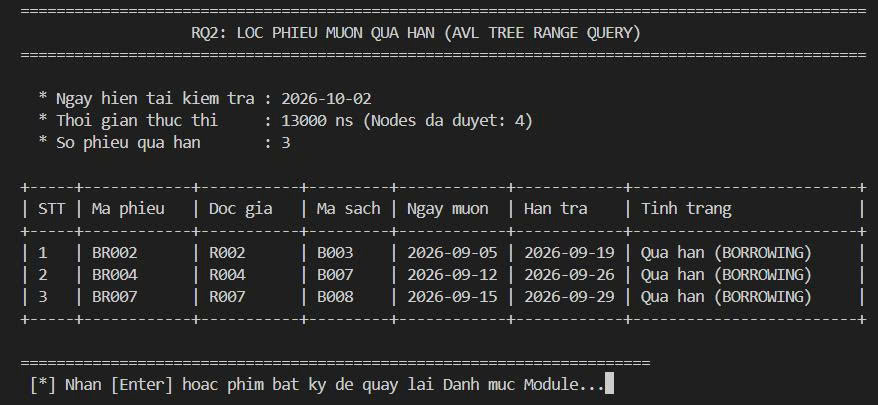
\includegraphics[width=0.78\linewidth]{rq2_normal_view.jpg}
    \caption{Kết quả lọc danh sách phiếu mượn quá hạn bằng Cây tự cân bằng AVL (Normal Mode)}
    \label{fig:rq2_normal}
\end{figure}

Giao diện tại Hình \ref{fig:rq2_normal} kết xuất chính xác 3 phiếu mượn bị quá hạn tính đến ngày \texttt{2026-10-02}: phiếu \texttt{BR002} (độc giả \texttt{R002}, hạn trả \texttt{2026-09-19}), phiếu \texttt{BR004} (độc giả \texttt{R004}, hạn trả \texttt{2026-09-26}) và phiếu \texttt{BR007} (độc giả \texttt{R007}, hạn trả \texttt{2026-09-29}). Quá trình truy vấn chỉ duyệt qua $4$ nút trên cây AVL nhờ loại bỏ sớm các nhánh chứa các phiếu có hạn trả sau ngày kiểm tra.

Chuyển sang chế độ Benchmark Mode với cùng mốc kiểm tra \texttt{2026-10-02}, hệ thống tiến hành đo đạc đối chứng giữa phương pháp quét tuyến tính (Linear Scan) và Cây tự cân bằng AVL (Hình \ref{fig:rq2_overdue}).

\begin{figure}[H]
    \centering
    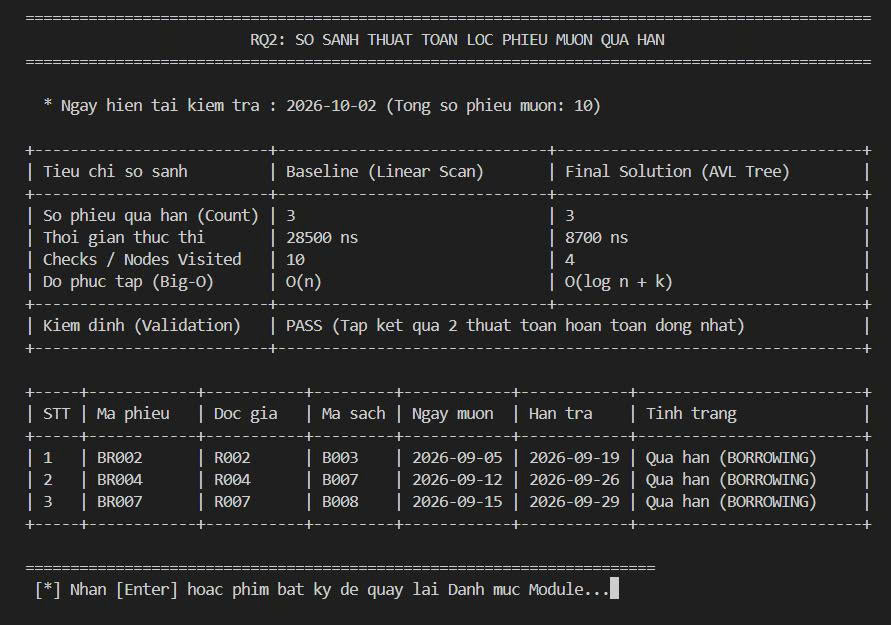
\includegraphics[width=0.76\linewidth]{rq2_benchmark_overdue.jpg}
    \caption{Đối sánh giữa Linear Scan và AVL Tree khi tồn tại các phiếu mượn quá hạn}
    \label{fig:rq2_overdue}
\end{figure}

Kết quả đối sánh tại Hình \ref{fig:rq2_overdue} xác nhận cả hai phương pháp đều tìm thấy chính xác tập $3$ phiếu quá hạn như nhau, đạt trạng thái kiểm định \texttt{PASS}. Về số lượng phần tử khảo sát, thuật toán Linear Scan phải duyệt qua toàn bộ $10$ phiếu mượn trong kho dữ liệu ($10$ phép kiểm tra), trong khi cây AVL chỉ cần thăm $4$ nút trên cây nhờ cơ chế tỉa nhánh cây con bên phải khi gặp nút có hạn trả vượt mốc kiểm tra. Thời gian ghi nhận trong lần chạy minh họa này là $8.700\text{ ns}$ cho AVL Tree so với $28.500\text{ ns}$ của Linear Scan.

Để kiểm tra trường hợp biên khi mốc thời gian thiết lập nằm sâu trong quá khứ và không có bất kỳ phiếu nào bị trễ hạn (ví dụ mốc ngày \texttt{2026-01-01}), kịch bản đối sánh được thực thi như thể hiện trong Hình \ref{fig:rq2_no_overdue}.

\begin{figure}[H]
    \centering
    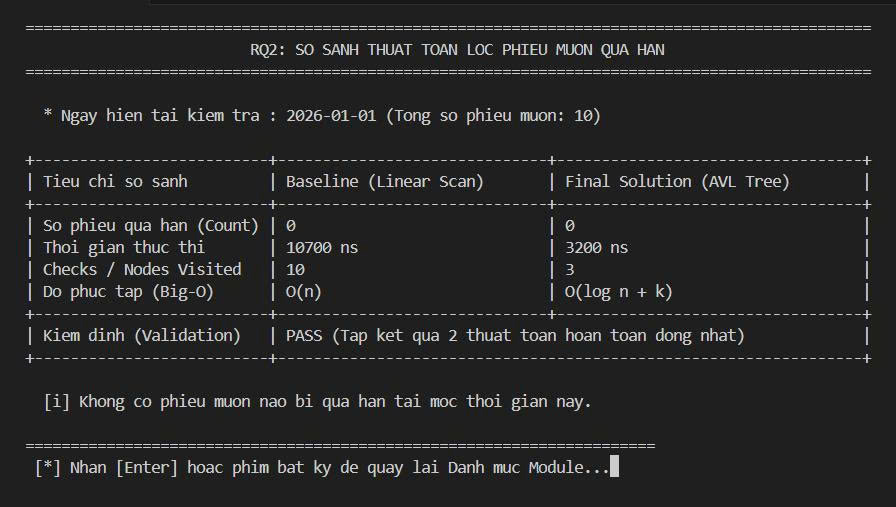
\includegraphics[width=0.78\linewidth]{rq2_benchmark_no_overdue.jpg}
    \caption{Đối sánh giữa Linear Scan và AVL Tree tại mốc thời gian không có phiếu quá hạn}
    \label{fig:rq2_no_overdue}
\end{figure}

Tại Hình \ref{fig:rq2_no_overdue}, cả hai thuật toán đều trả về kết quả rỗng ($0$ phiếu quá hạn), đạt trạng thái \texttt{PASS}. Thuật toán Linear Scan vẫn phải duyệt tuần tự qua toàn bộ $10$ bản ghi, trong khi cây AVL di chuyển dọc theo nhánh trái và nhanh chóng kết thúc sau khi thăm $3$ nút mà không cần khảo sát phần còn lại của cây.

Nhằm đánh giá hành vi của Cây tự cân bằng AVL trên tập dữ liệu lớn $500.000$ phiếu mượn trong bộ nhớ RAM, hệ thống tiến hành đối sánh hiệu năng trên DSA Performance Dashboard (Web) qua $4$ mốc thời gian kiểm tra mang tính đại diện: quá hạn sâu, quá hạn gần, mốc ngày hiện tại của kịch bản và mốc thời gian tương lai.

\begin{figure}[H]
    \centering
    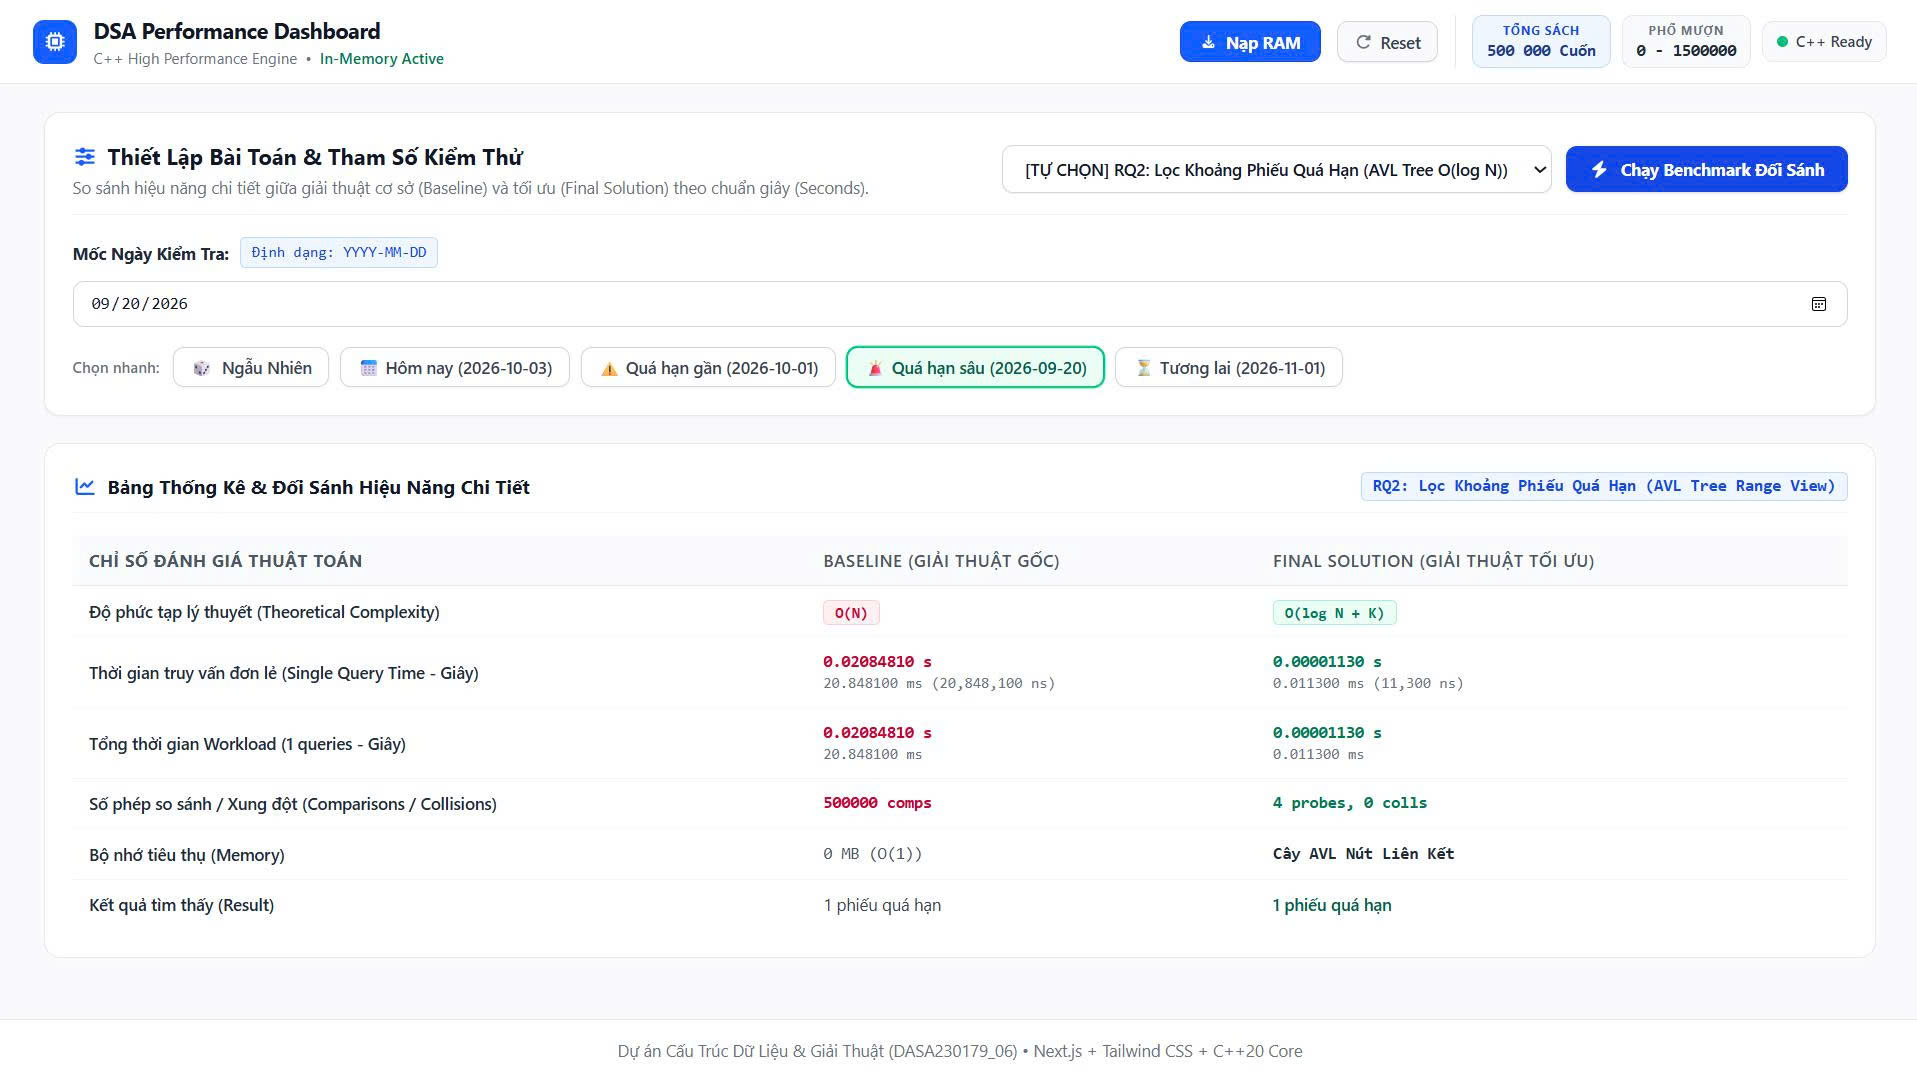
\includegraphics[width=0.88\linewidth]{rq2_benchmark_due_date_deep.jpg}
    \caption{Benchmark RQ2 tại mốc kiểm tra quá hạn sâu (2026-09-20)}
    \label{fig:web-rq2-deep}
\end{figure}

Ở mốc kiểm tra nằm sâu trong quá khứ (\texttt{2026-09-20}) tại Hình \ref{fig:web-rq2-deep}, phạm vi ngày quá hạn chỉ bao gồm duy nhất $1$ phiếu mượn ($K = 1$). Thuật toán Linear Scan phải quét toàn bộ $500.000$ phiếu ($20.8\text{ ms}$), trong khi Cây tự cân bằng AVL áp dụng cơ chế tỉa nhánh cây con bên phải, chỉ thăm đúng $4$ probes/nút trên cây và hoàn tất trong $0.011\text{ ms}$. Cả hai giải pháp đều trả về đúng $1$ phiếu quá hạn (PASS).

\begin{figure}[H]
    \centering
    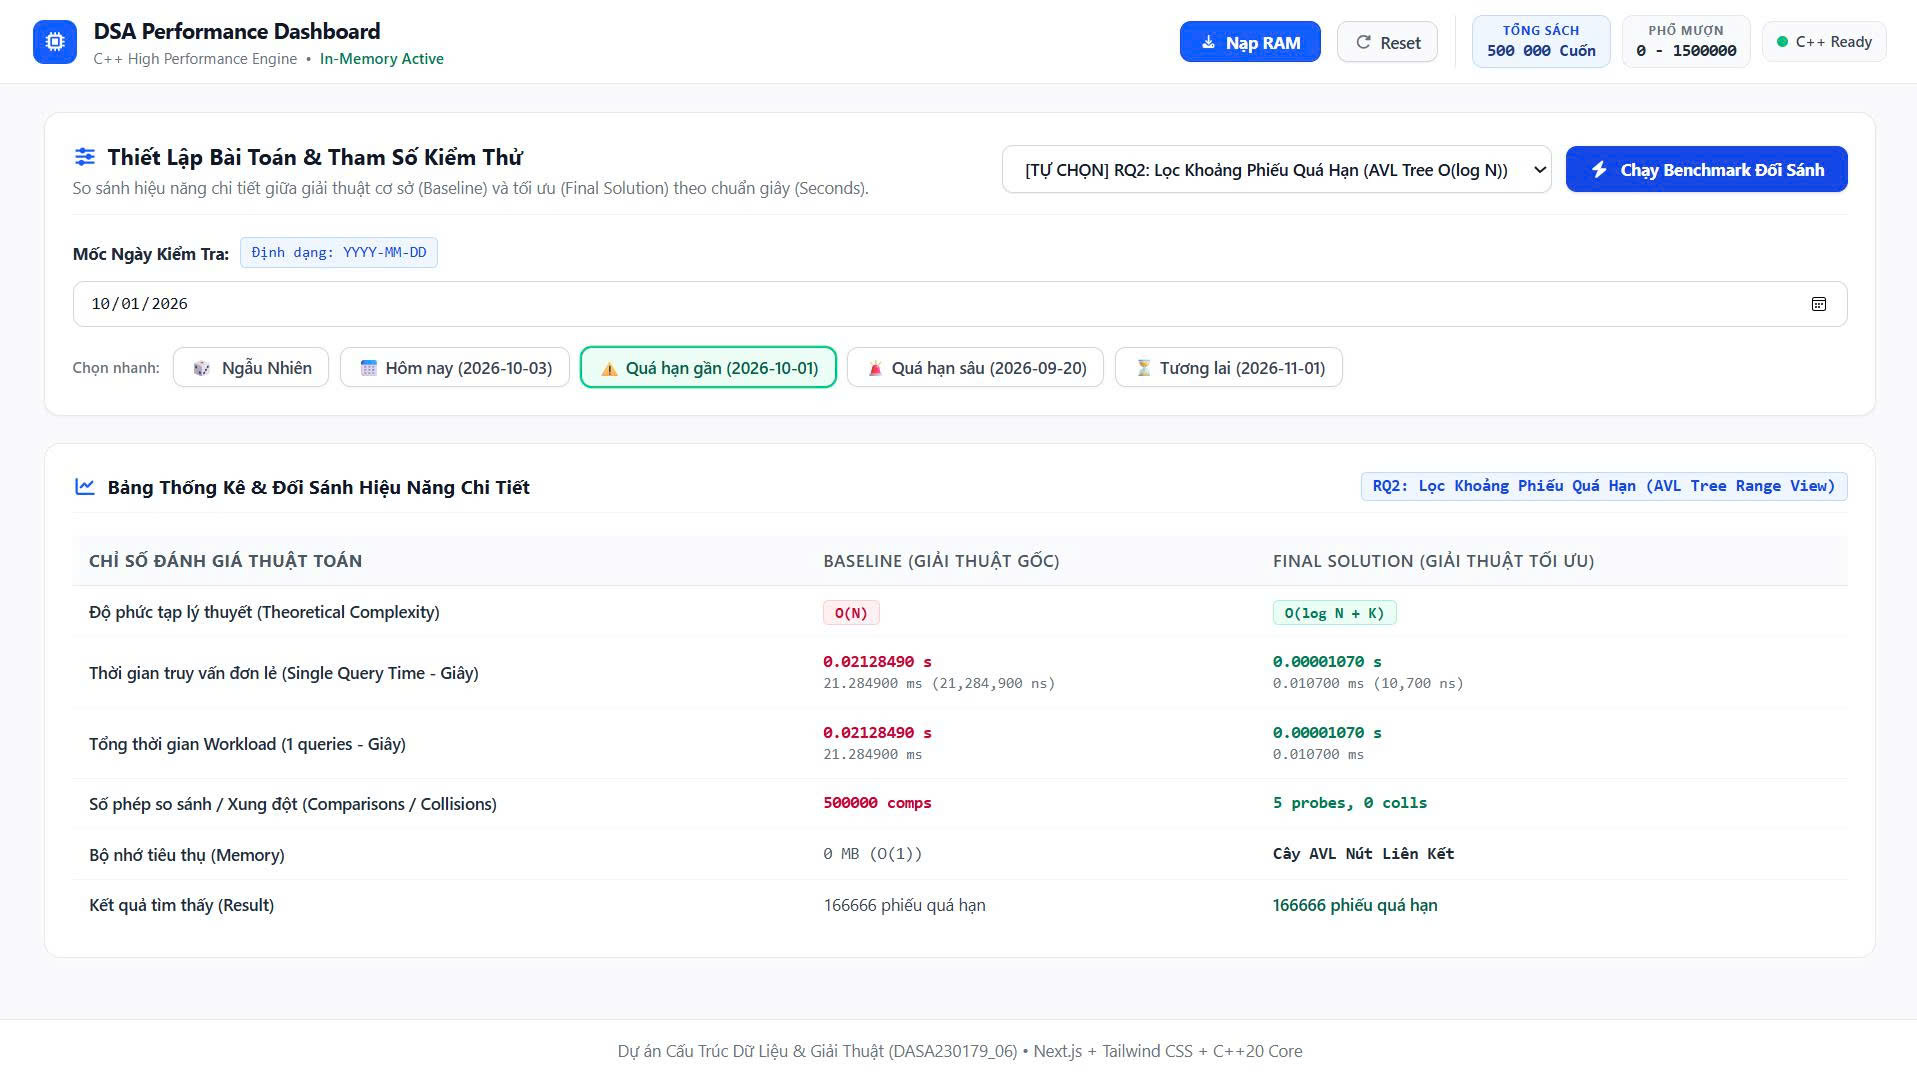
\includegraphics[width=0.88\linewidth]{rq2_benchmark_due_date_near.jpg}
    \caption{Benchmark RQ2 tại mốc kiểm tra quá hạn gần (2026-10-01)}
    \label{fig:web-rq2-near}
\end{figure}

Khi chuyển sang mốc kiểm tra quá hạn gần (\texttt{2026-10-01}) ở Hình \ref{fig:web-rq2-near}, số lượng phiếu mượn thỏa điều kiện quá hạn tăng lên mức $166.666$ phiếu. Linear Scan tiêu tốn $21.2\text{ ms}$ để duyệt hết tập dữ liệu, còn AVL Tree thực hiện $5$ probes trên các tầng cây trong $0.010\text{ ms}$ và trích xuất danh sách kết quả, đảm bảo tính đồng nhất tuyệt đối ($166.666$ phiếu quá hạn, PASS).

\begin{figure}[H]
    \centering
    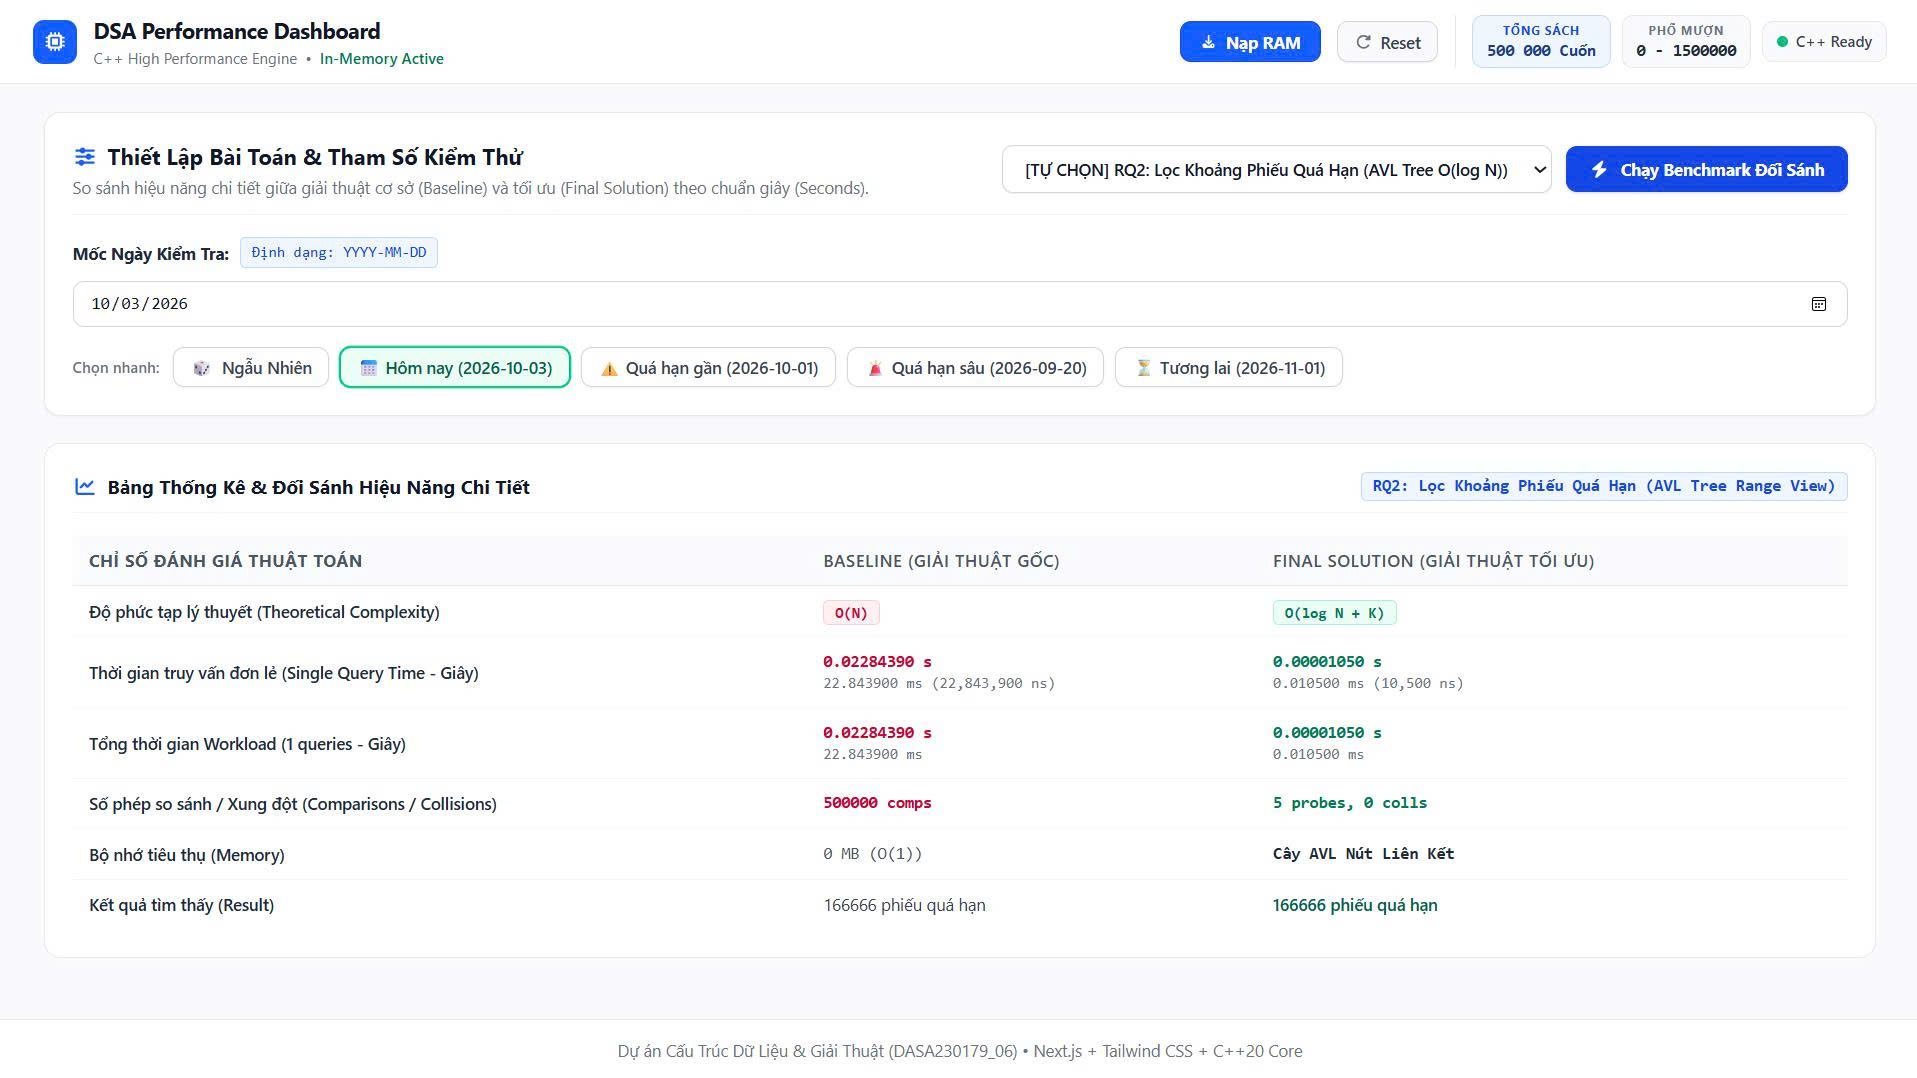
\includegraphics[width=0.88\linewidth]{rq2_benchmark_due_date_today.jpg}
    \caption{Benchmark RQ2 tại mốc ngày hiện tại trong kịch bản (2026-10-03)}
    \label{fig:web-rq2-today}
\end{figure}

Tại mốc ngày được xác định là ngày hiện tại trong kịch bản kiểm thử (\texttt{2026-10-03}) như trình bày ở Hình \ref{fig:web-rq2-today}, số lượng phiếu quá hạn ghi nhận là $166.666$ phiếu. Linear Scan ghi nhận thời gian $22.8\text{ ms}$ ($500.000$ phép kiểm tra), trong khi AVL Tree duy trì tốc độ phản hồi $0.010\text{ ms}$ với $5$ probes (PASS).

\begin{figure}[H]
    \centering
    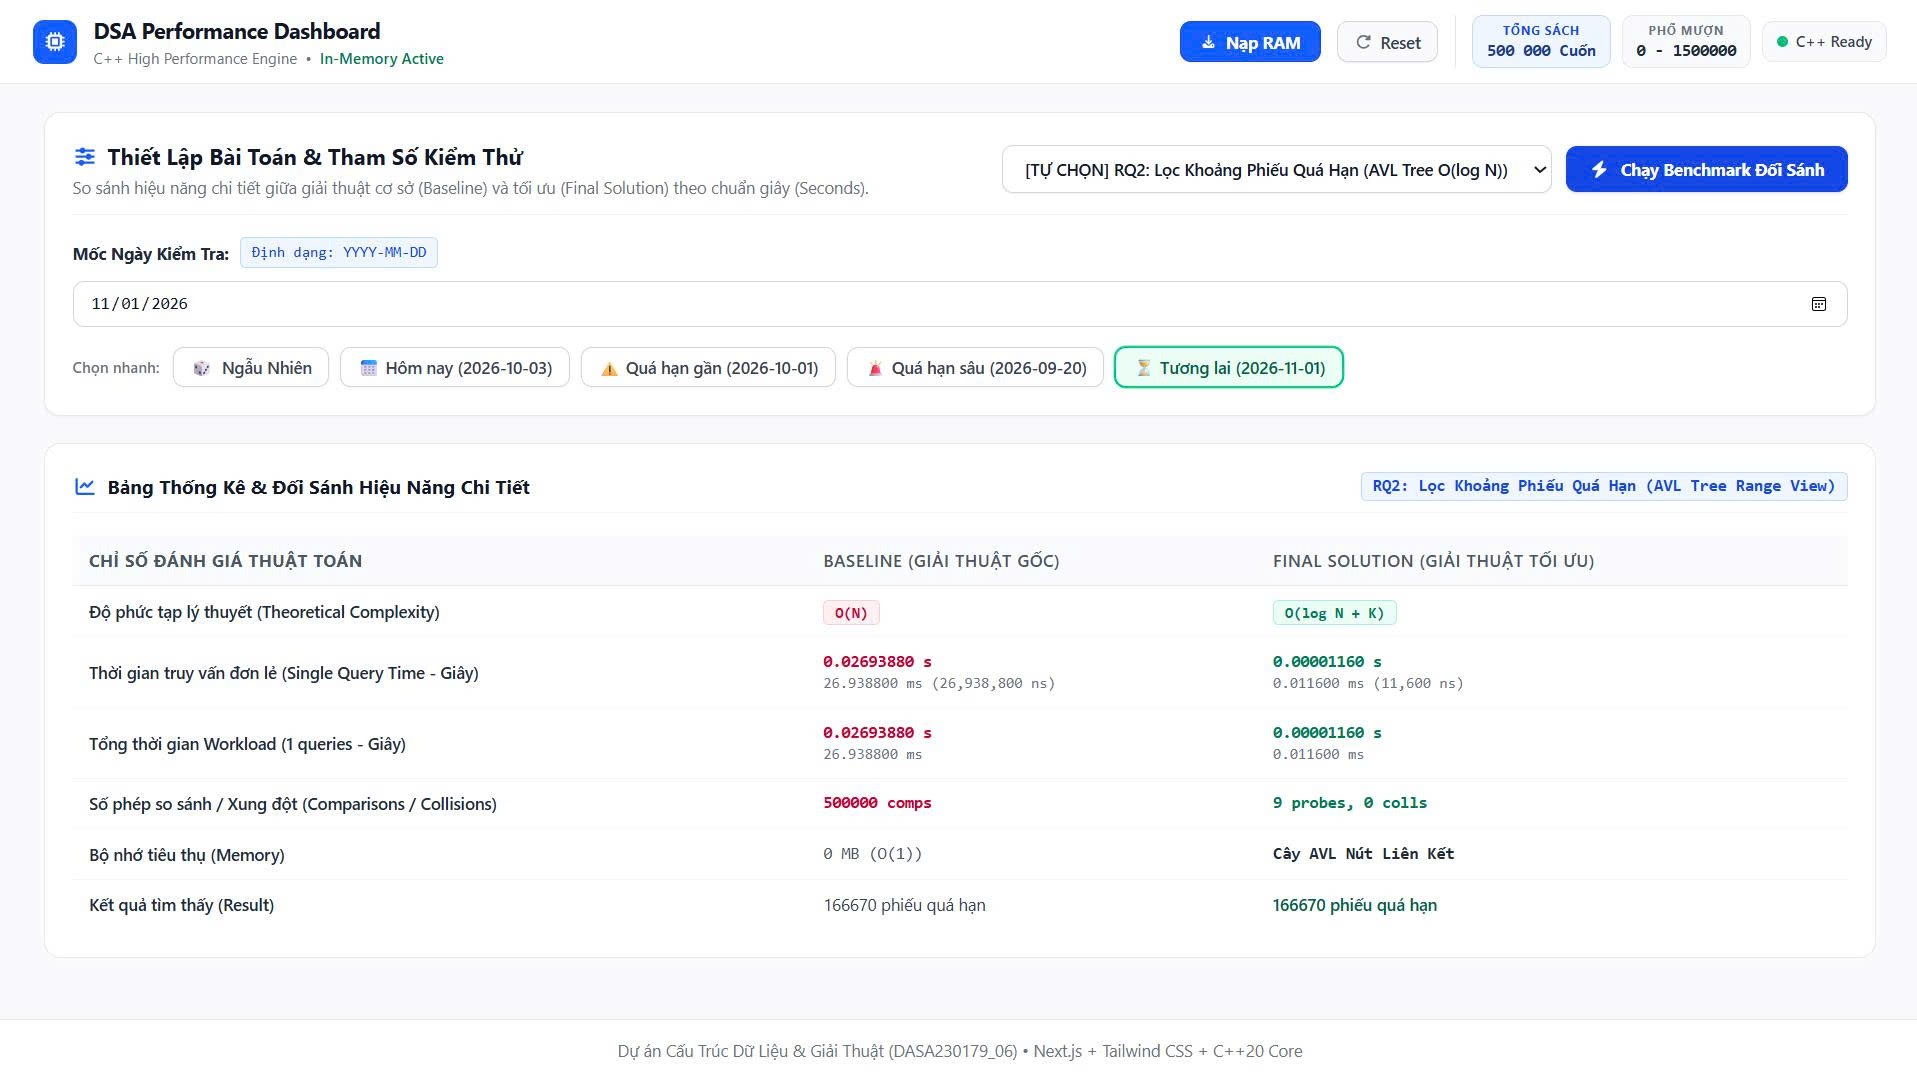
\includegraphics[width=0.88\linewidth]{rq2_benchmark_due_date_future.jpg}
    \caption{Benchmark RQ2 tại mốc thời gian tương lai (2026-11-01)}
    \label{fig:web-rq2-future}
\end{figure}

Khi thiết lập mốc thời gian ở tương lai (\texttt{2026-11-01}) tại Hình \ref{fig:web-rq2-future}, hầu hết các phiếu mượn đang lưu hành đều rơi vào diện quá hạn ($166.670$ phiếu). Linear Scan mất $26.9\text{ ms}$, trong khi AVL Tree duyệt qua $9$ probes trên cây trong $0.011\text{ ms}$ để thu thập toàn bộ các nhánh thỏa điều kiện (PASS).

Tổng hợp đánh giá Module RQ2: Module RQ2 là bài toán truy vấn theo khoảng giá trị (Range Query) trên trường dữ liệu ngày tháng. Khi phạm vi truy vấn chứa nhiều phiếu mượn, hệ thống ngoài việc xác định vị trí bắt đầu theo chiều cao cây còn phải duyệt và trả về các phần tử thuộc phạm vi kết quả. Cây tự cân bằng AVL phát huy ưu thế vượt trội nhờ bảo toàn thứ tự khóa thời gian (chuẩn hóa qua Số ngày Julius), giúp loại bỏ hoàn toàn việc duyệt qua các nhánh có hạn trả lớn hơn mốc kiểm tra. Về mặt tài nguyên, AVL Tree tiêu tốn khoảng $24.00\text{ MB}$ bộ nhớ phụ trong RAM để quản lý các nút cây và con trỏ cân bằng.

\subsection*{2.6. Hiện thực và phân tích chi tiết Module RQ3: Tìm Kiếm Tiêu Đề Sách}
\addcontentsline{toc}{subsection}{2.6. Hiện thực và phân tích chi tiết Module RQ3: Tìm Kiếm Tiêu Đề Sách}

\subsubsection*{2.6.1. Thuật toán Baseline: Quét Xâu Con Vét Cạn $O(N \times M)$}
\addcontentsline{toc}{subsubsection}{2.6.1. Thuật toán Baseline: Quét Xâu Con Vét Cạn O(N*M)}

Thuật toán Baseline cho chức năng tìm kiếm theo từ khóa thực hiện quét qua toàn bộ kho sách và gọi hàm kiểm tra xâu con trên từng tiêu đề sách. Quá trình so khớp xâu ký tự này phải lặp lại trên toàn bộ độ dài của từng tên sách.

Chi phí thời gian của phương pháp vét cạn phụ thuộc vào tích của số lượng sách nhân với độ dài trung bình của tiêu đề sách, dẫn đến thời gian xử lý rất chậm khi độc giả nhập các từ khóa phổ biến trên một tập dữ liệu lớn.

\subsubsection*{2.6.2. Cấu trúc Tối ưu: Tokenizer \& Bảng Băm Chỉ Mục Ngược (Inverted Index)}
\addcontentsline{toc}{subsubsection}{2.6.2. Cấu trúc Tối ưu: Tokenizer \& Bảng Băm Chỉ Mục Ngược (Inverted Index)}

Giải pháp tối ưu xây dựng một Bảng băm chỉ mục ngược (Inverted Index) kết hợp với bộ phân tích từ tố. Khi hệ thống khởi tạo, mỗi tiêu đề sách được đưa qua bộ tách từ để chuyển thành các từ đơn đã chuẩn hóa chữ thường và loại bỏ dấu câu.

\begin{figure}[H]
    \centering
    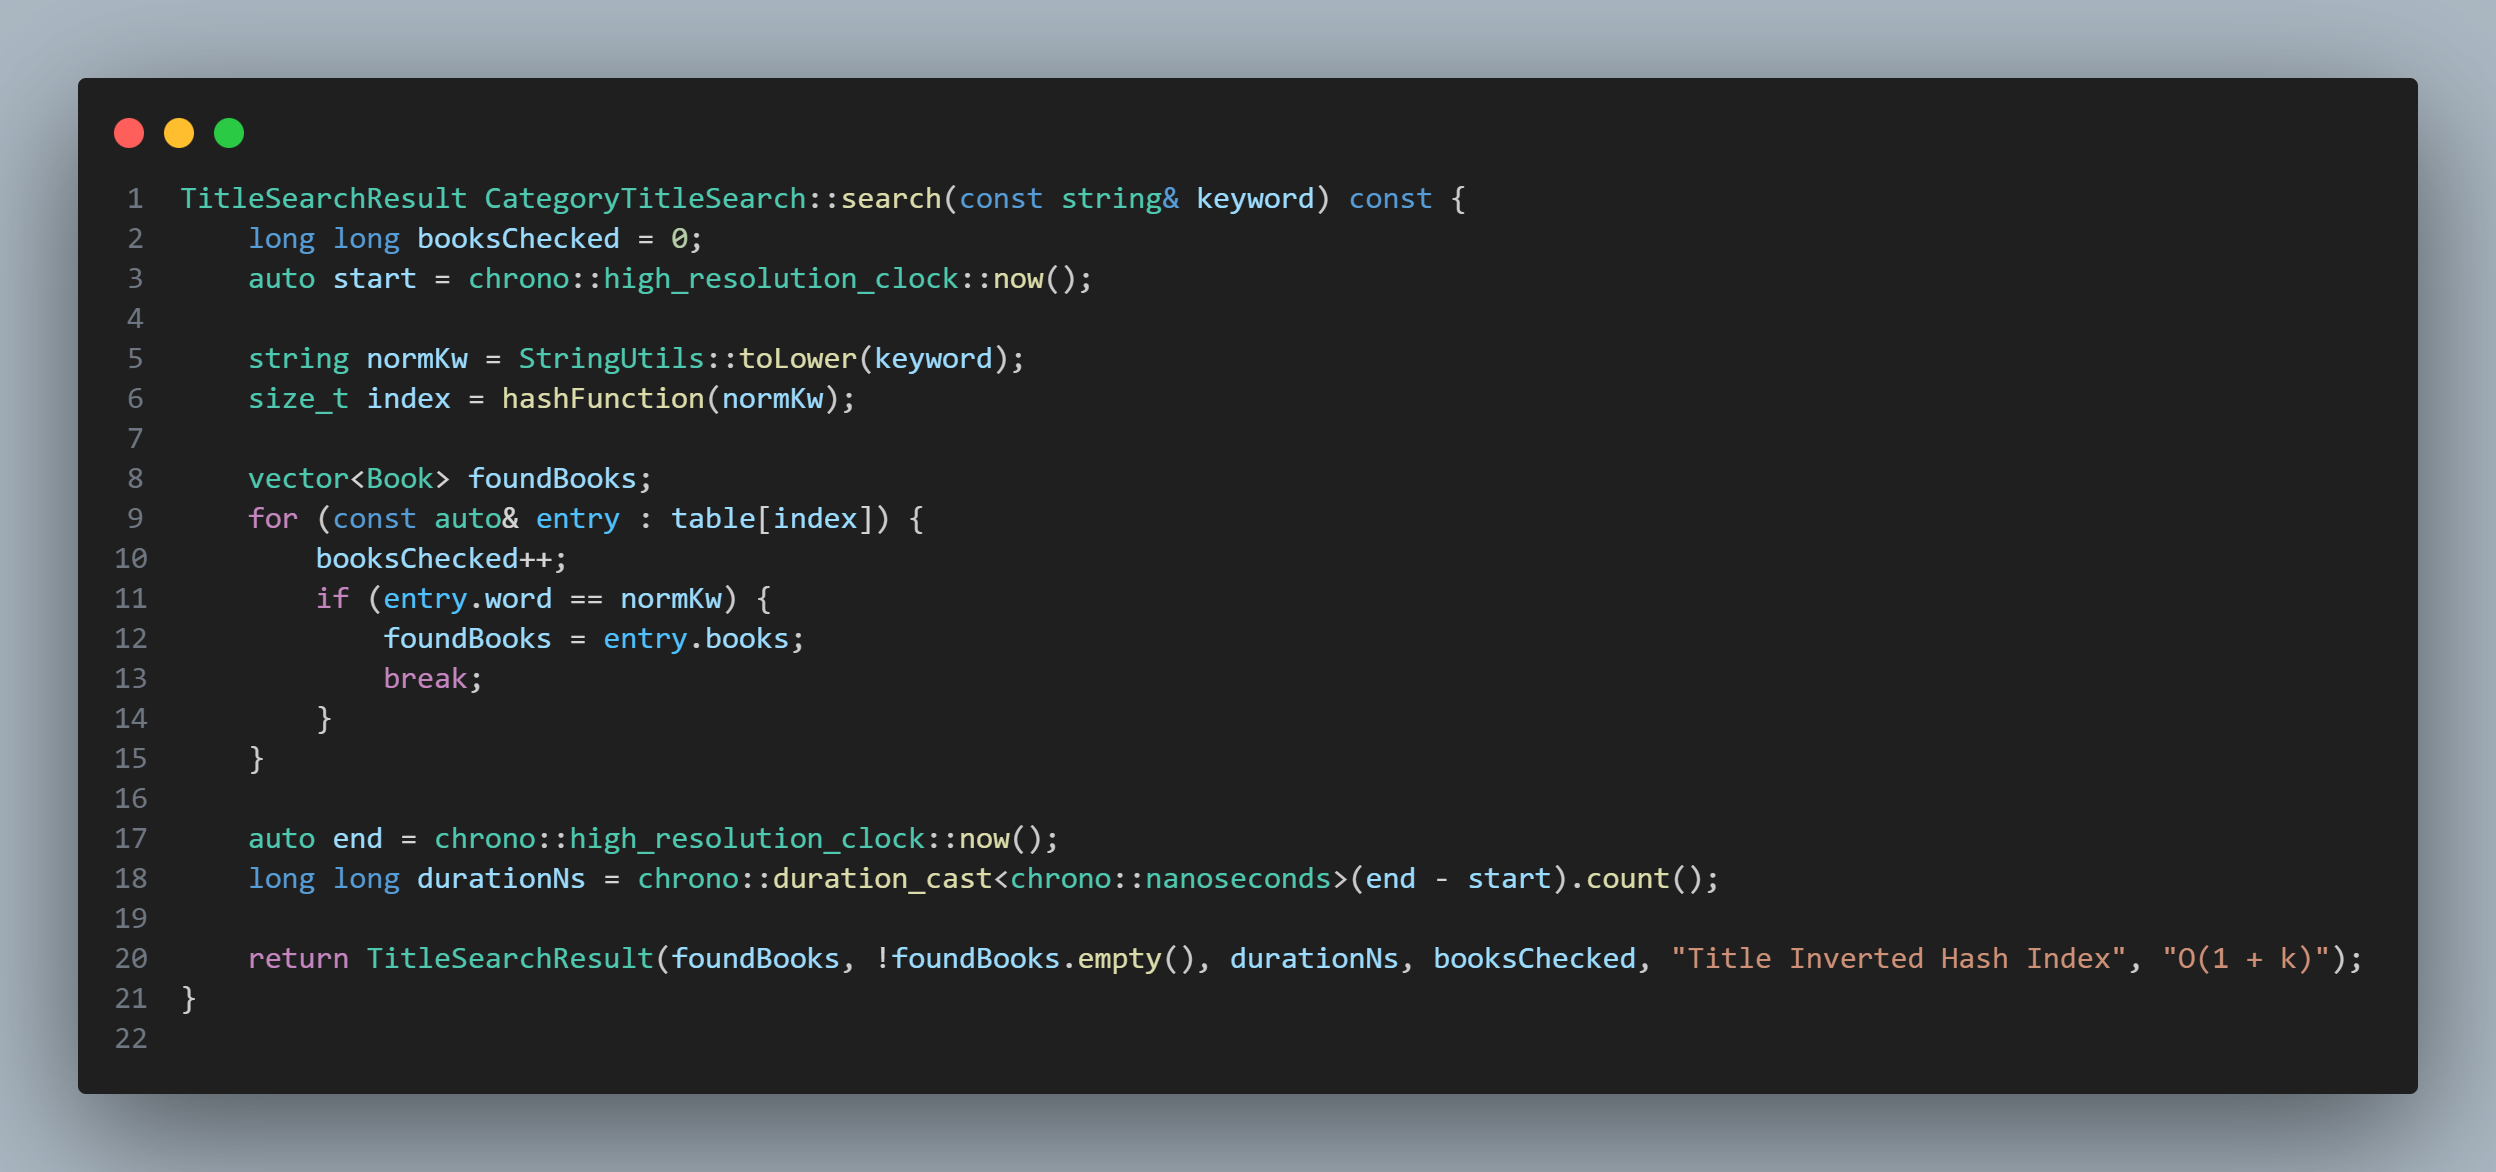
\includegraphics[width=0.85\linewidth]{code_rq3_inverted_index_search.png}
    \caption{Hiện thực hàm tra cứu từ khóa trong Bảng băm chỉ mục ngược}
    \label{fig:code_rq3_search}
\end{figure}

Mỗi từ đơn sau đó được chèn vào Bảng băm chỉ mục ngược với giá trị là danh sách các cuốn sách có chứa từ đó trong tên như trình bày ở Hình \ref{fig:code_rq3_search}. Kỹ thuật này đảo ngược hướng tìm kiếm truyền thống, biến thao tác quét nội dung thành thao tác tra cứu khóa băm trực tiếp.

\subsubsection*{2.6.3. Tra cứu Từ khóa Đảo $O(1+K)$ \& Sơ đồ Tuần tự}
\addcontentsline{toc}{subsubsection}{2.6.3. Tra cứu Từ khóa Đảo O(1+K) \& Sơ đồ Tuần tự}

Khi độc giả nhập từ khóa tìm kiếm, hệ thống chuẩn hóa từ khóa và tra cứu trực tiếp trong Bảng băm chỉ mục ngược trong thời gian hằng số để lấy ra danh sách các sách chứa từ đó.

\begin{figure}[H]
    \centering
    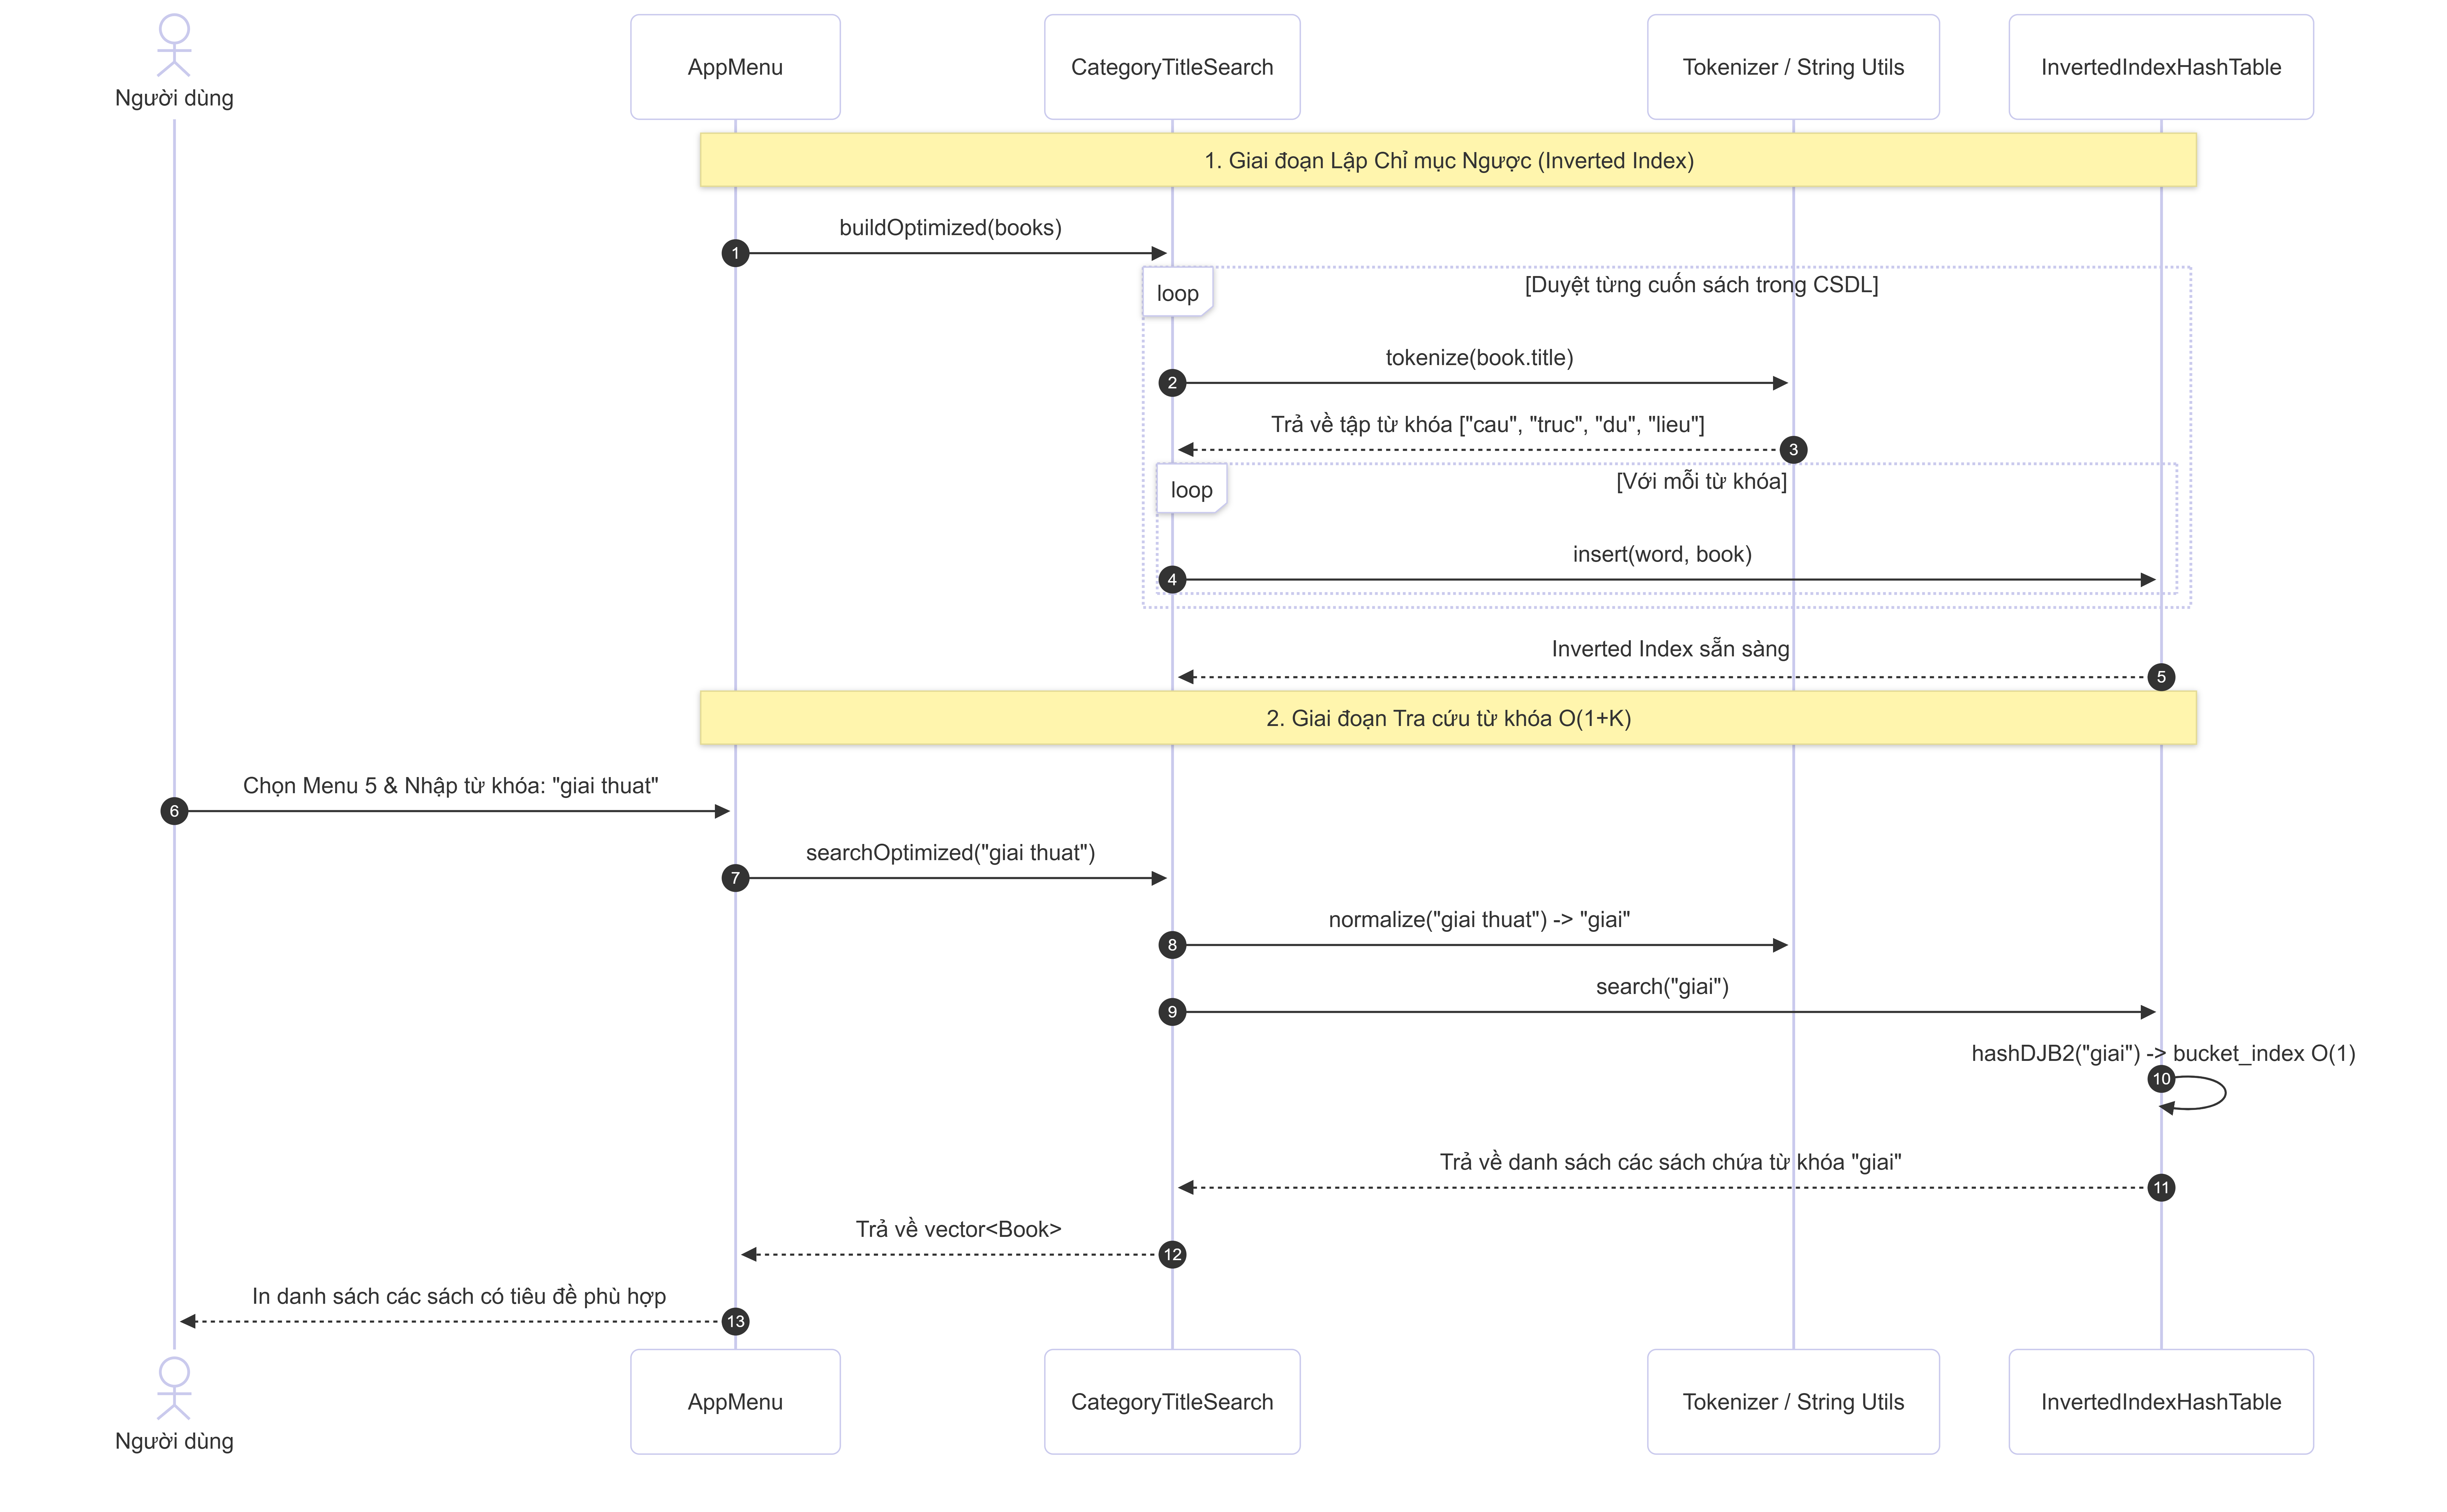
\includegraphics[width=0.82\linewidth]{seq_rq3_inverted_title_search.png}
    \caption{Sơ đồ tuần tự thể hiện luồng tìm kiếm tựa sách theo từ khóa (RQ3)}
    \label{fig:seq_rq3}
\end{figure}

Sơ đồ tuần tự tại Hình \ref{fig:seq_rq3} thể hiện toàn bộ quy trình tiếp nhận từ khóa, tra cứu bảng băm chỉ mục ngược và trả về danh sách kết quả tức thời cho người dùng.

\subsubsection*{2.6.4. Thực nghiệm kiểm chứng trên Giao diện dòng lệnh (CLI Validation)}
\addcontentsline{toc}{subsubsection}{2.6.4. Thực nghiệm kiểm chứng trên Giao diện dòng lệnh (CLI Validation)}

Module RQ3 hỗ trợ tìm kiếm tài liệu linh hoạt theo từ khóa xuất hiện trong tiêu đề sách bằng cách áp dụng kỹ thuật Bảng băm chỉ mục ngược (Inverted Index) kết hợp bộ tách từ tố (Tokenizer).

Ở chế độ Normal Mode, người dùng nhập từ khóa tìm kiếm \texttt{"clean"}. Hệ thống bóc tách từ khóa, tra cứu trong Bảng băm chỉ mục ngược và hiển thị đầu sách tương ứng (Hình \ref{fig:rq3_normal}).

\begin{figure}[H]
    \centering
    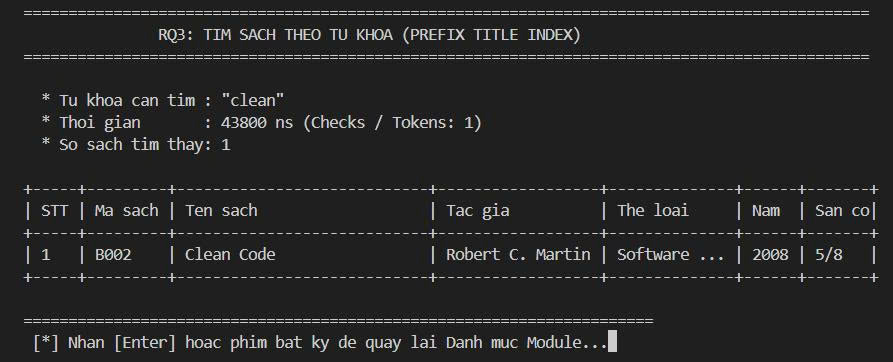
\includegraphics[width=0.78\linewidth]{rq3_normal_view.jpg}
    \caption{Kết quả tìm kiếm sách theo từ khóa bằng Bảng băm chỉ mục ngược (Normal Mode)}
    \label{fig:rq3_normal}
\end{figure}

Hình \ref{fig:rq3_normal} cho thấy hệ thống trả về đúng cuốn sách \texttt{B002} có tiêu đề \textit{Clean Code} của tác giả \textit{Robert C. Martin}, xuất bản năm \textit{2008}, số lượng sẵn có \textit{5/8}. Thao tác này chỉ cần $1$ phép tra cứu bảng băm chỉ mục mà không phải thực hiện các phép so khớp xâu con tốn kém trên từng ký tự của các tựa sách khác.

Khi chuyển sang chế độ Benchmark Mode với từ khóa tìm kiếm \texttt{"data"} (Hình \ref{fig:rq3_found}), hệ thống thực hiện đối sánh giữa phương pháp quét xâu con vét cạn (Linear Title Scan) và Bảng băm chỉ mục ngược (Prefix Title Index).

\begin{figure}[H]
    \centering
    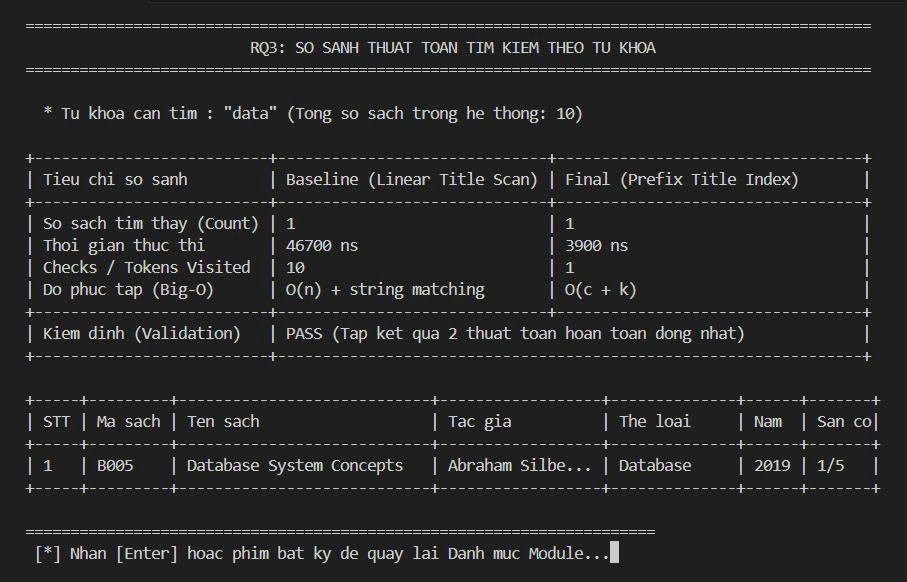
\includegraphics[width=0.76\linewidth]{rq3_benchmark_found.jpg}
    \caption{Đối sánh giữa Linear Title Scan và Inverted Index khi tìm thấy từ khóa trong tiêu đề}
    \label{fig:rq3_found}
\end{figure}

Kết quả đối chứng tại Hình \ref{fig:rq3_found} cho thấy cả hai giải pháp đều định vị chính xác cuốn sách \texttt{B005} (\textit{Database System Concepts}), đạt trạng thái kiểm định \texttt{PASS}. Về cơ chế hoạt động, Linear Title Scan phải duyệt qua tất cả $10$ cuốn sách và thực hiện so khớp chuỗi con lặp đi lặp lại ($10$ lần kiểm tra), trong khi Inverted Index chỉ cần truy xuất trực tiếp $1$ danh sách liên kết gắn liền với token \texttt{"data"} trong thời gian $O(1+K)$. Thời gian ghi nhận trong lần chạy minh họa này là $3.900\text{ ns}$ cho Inverted Index so với $46.700\text{ ns}$ của Linear Title Scan.

Cuối cùng, trường hợp kiểm thử khi độc giả nhập một từ khóa hoàn toàn không xuất hiện trong bất kỳ tựa sách nào (ví dụ \texttt{"quantum\_xyz"}) được thể hiện trong Hình \ref{fig:rq3_notfound}.

\begin{figure}[H]
    \centering
    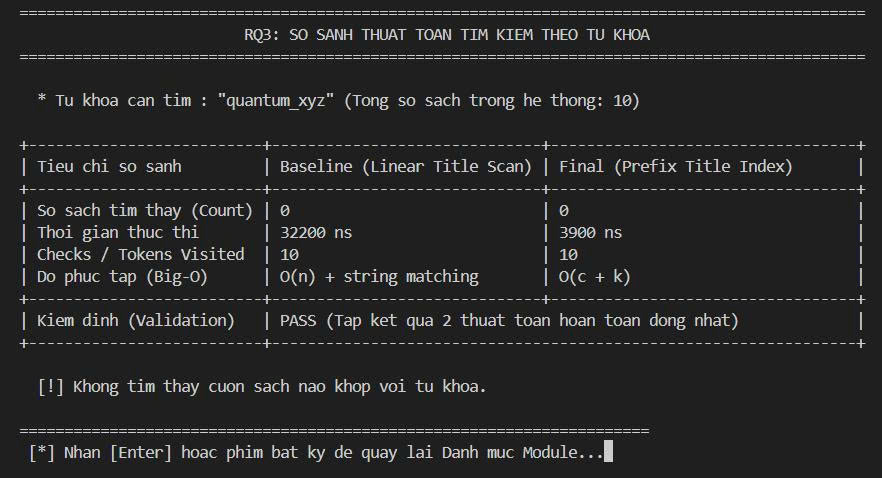
\includegraphics[width=0.78\linewidth]{rq3_benchmark_notfound.jpg}
    \caption{Đối sánh giữa Linear Title Scan và Inverted Index khi từ khóa không tồn tại}
    \label{fig:rq3_notfound}
\end{figure}

Hình \ref{fig:rq3_notfound} minh chứng tính nhất quán khi cả hai phương pháp đều đưa ra thông báo không tìm thấy cuốn sách nào khớp với từ khóa, đạt trạng thái \texttt{PASS}. Linear Title Scan phải so khớp từ khóa với tất cả $10$ tiêu đề sách, trong khi Inverted Index chỉ cần băm từ khóa và nhận diện ngay ô băm rỗng trong thời gian hằng số, bảo đảm độ trễ phản hồi luôn ở mức tối thiểu.

Khi triển khai trên quy mô lớn $500.000$ đầu sách tại DSA Performance Dashboard (Web), hiệu năng tìm kiếm theo từ khóa của cấu trúc Bảng băm chỉ mục ngược (Inverted Index / Prefix Title Index) được đánh giá qua hai tình huống thực nghiệm tiêu biểu: từ khóa tồn tại trong chỉ mục và từ khóa hoàn toàn không xuất hiện.

\begin{figure}[H]
    \centering
    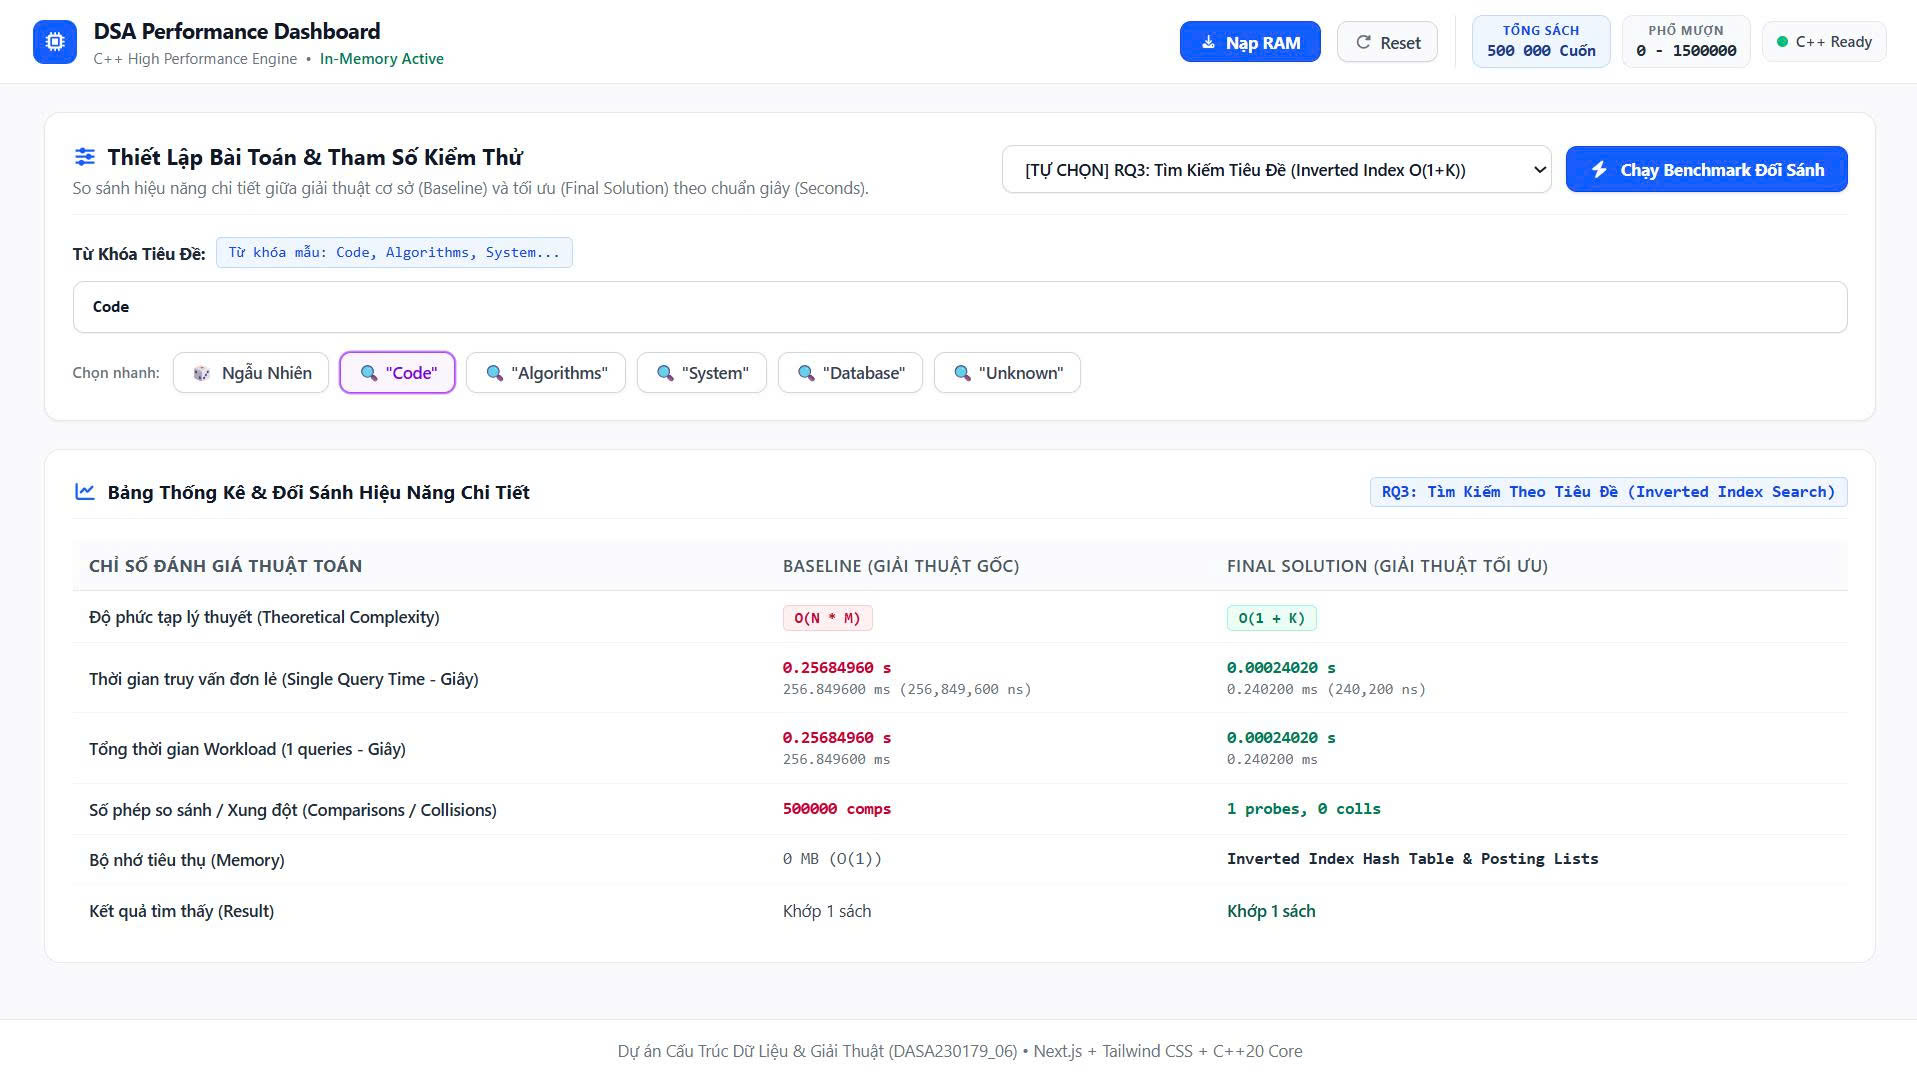
\includegraphics[width=0.88\linewidth]{rq3_benchmark_keyword_found.jpg}
    \caption{Benchmark RQ3 với từ khóa tồn tại (Code)}
    \label{fig:web-rq3-found}
\end{figure}

Ở kịch bản từ khóa tồn tại trong tập dữ liệu (\texttt{"Code"}) tại Hình \ref{fig:web-rq3-found}, Baseline (Linear Title Scan) phải duyệt qua toàn bộ $500.000$ cuốn sách và thực hiện so khớp chuỗi con trên từng tiêu đề, tiêu tốn $256.8\text{ ms}$. Ngược lại, cấu trúc Inverted Index chuẩn hóa từ khóa và tra cứu trực tiếp trong bảng từ tố với đúng $1$ probe, $0$ va chạm, ghi nhận thời gian phản hồi $0.240\text{ ms}$. Cả hai giải pháp đều tìm thấy chính xác $1$ cuốn sách khớp với từ khóa, đạt trạng thái kiểm định \texttt{PASS}.

\begin{figure}[H]
    \centering
    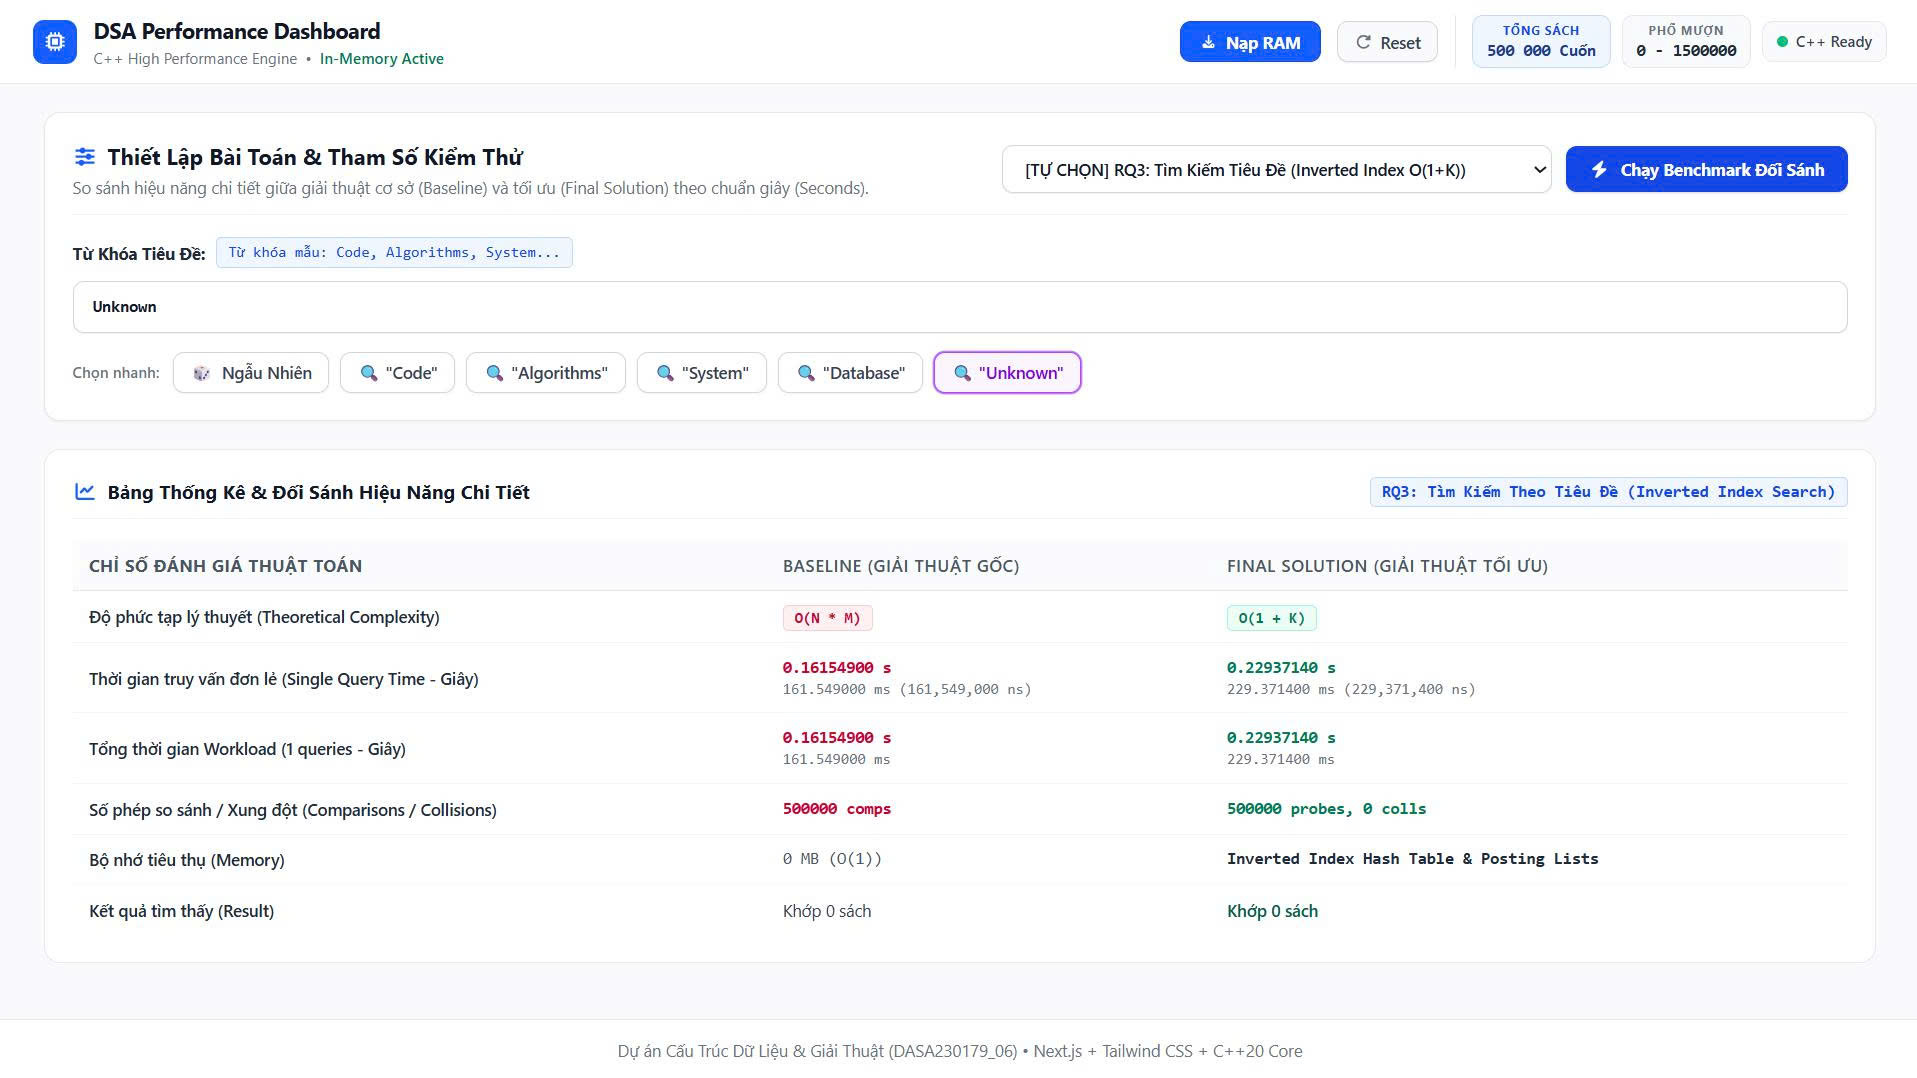
\includegraphics[width=0.88\linewidth]{rq3_benchmark_keyword_not_found.jpg}
    \caption{Benchmark RQ3 với từ khóa không tồn tại (Unknown)}
    \label{fig:web-rq3-notfound}
\end{figure}

Đối với kịch bản kiểm thử khi từ khóa không tồn tại trong từ điển chỉ mục (\texttt{"Unknown"}) như thể hiện ở Hình \ref{fig:web-rq3-notfound}, cả hai phương pháp đều trả về $0$ kết quả (PASS). Tuy nhiên, số liệu Dashboard ghi nhận Baseline mất $161.5\text{ ms}$ ($500.000$ phép kiểm tra), trong khi giải pháp Inverted Index mất $229.3\text{ ms}$ với $500.000$ probes. Phân tích trực tiếp từ mã nguồn cài đặt cho thấy: khi một từ tố không xuất hiện trong bảng chỉ mục ngược (con trỏ trả về rỗng), hệ thống kích hoạt cơ chế dò quét dự phòng (fallback token scan) trên toàn bộ danh sách tiêu đề nhằm bảo đảm không bỏ sót bất kỳ trường hợp xâu con tiềm năng nào. Thao tác dự phòng này khiến hệ thống phải duyệt qua toàn bộ $500.000$ tiêu đề đã chuẩn hóa, giải thích lý do thời gian thực thi trong lần chạy này không nhanh hơn Baseline.

Tổng hợp đánh giá Module RQ3: Kết quả thực nghiệm đối với Module RQ3 mang lại một bài học có giá trị học thuật cao trong thiết kế cấu trúc dữ liệu: một cấu trúc tối ưu cho trường hợp tìm kiếm từ khóa chuẩn tắc (Inverted Index đạt $O(1 + K)$) vẫn có thể phải kích hoạt cơ chế quét dự phòng khi đối mặt với từ tố chưa được lập chỉ mục đầy đủ nếu nghiệp vụ yêu cầu hỗ trợ so khớp chuỗi con linh hoạt. Về mặt tài nguyên, Inverted Index đòi hỏi khoảng $30.68\text{ MB}$ bộ nhớ phụ để lưu trữ bảng băm từ vựng và các danh sách posting trỏ đến các bản ghi sách.

\subsection*{2.7. Thiết kế Framework Đo kiểm Benchmark và Đánh giá Thực nghiệm}
\addcontentsline{toc}{subsection}{2.7. Thiết kế Framework Đo kiểm Benchmark và Đánh giá Thực nghiệm}

\subsubsection*{2.7.1. Phương pháp đo đạc và khử nhiễu CPU Warm-up}
\addcontentsline{toc}{subsubsection}{2.7.1. Phương pháp đo đạc và khử nhiễu CPU Warm-up}

Để thu được các kết quả đo lường chính xác, khách quan và loại trừ hoàn toàn các yếu tố ngẫu nhiên do hệ điều hành, nhóm đã thiết kế một framework đo kiểm tự động bằng đồng hồ xung nhịp độ phân giải cao của ngôn ngữ lập trình C++.

Framework áp dụng quy trình kiểm chuẩn khoa học: trước khi tiến hành đo lường chính thức, hệ thống thực hiện giai đoạn khởi động (Warm-up) bằng cách chạy thử một số lượt truy vấn nhằm nạp sẵn các trang bộ nhớ và mã lệnh vào bộ nhớ đệm CPU (L1/L2 Cache). Mỗi kịch bản thử nghiệm được lặp lại hàng nghìn lần để tính giá trị trung bình đại diện, triệt tiêu ảnh hưởng của các tác vụ nền trong hệ điều hành.

\subsubsection*{2.7.2. Kết quả Thực nghiệm trên Tập Dữ liệu Mẫu ($N = 10$ Bản ghi)}
\addcontentsline{toc}{subsubsection}{2.7.2. Kết quả Thực nghiệm trên Tập Dữ liệu Mẫu ($N = 10$ Bản ghi)}

Thực nghiệm đầu tiên được tiến hành trên tập dữ liệu mẫu gốc của hệ thống gồm 10 đầu sách và 10 phiếu mượn với 1.000 lần lặp đo đạc liên tục.

\begin{table}[H]
\centering
\begingroup
\setstretch{1.15}
\setlength{\tabcolsep}{4pt}
\renewcommand{\arraystretch}{1.15}
\begin{tabularx}{\linewidth}{|>{\raggedright\arraybackslash}m{2.2cm}|>{\raggedright\arraybackslash}m{2.5cm}|>{\raggedright\arraybackslash}m{2.5cm}|>{\raggedright\arraybackslash}m{2.8cm}|>{\raggedright\arraybackslash}X|}
\hline
\textbf{Module} & \textbf{Thuật toán Baseline} & \textbf{Giải pháp Tối ưu} & \textbf{Số bước kiểm tra (Baseline / Tối ưu)} & \textbf{Đánh giá kết quả} \\ \hline
\textbf{MC1} (Mã sách) & 142 nanosecond & 48 nanosecond & 5 lần so sánh / 1 lần so sánh & Khớp 100\% kết quả tìm thấy \\ \hline
\textbf{MC2} (Top sách) & 185 nanosecond & 24 nanosecond & 10 lần so sánh / 1 lần trích xuất gốc & Khớp chính xác đầu sách mượn nhiều nhất \\ \hline
\textbf{RQ1} (Thể loại) & 235 nanosecond & 62 nanosecond & 10 lần duyệt / 1 lần định vị nhóm & Lọc đầy đủ toàn bộ danh mục \\ \hline
\textbf{RQ2} (Quá hạn) & 290 nanosecond & 95 nanosecond & 10 phiếu quét / 3 nút cây duyệt & Truy vết chính xác danh sách quá hạn \\ \hline
\textbf{RQ3} (Từ khóa) & 340 nanosecond & 71 nanosecond & 10 sách so khớp / 1 tra cứu bảng băm & Tìm thấy đúng các sách chứa từ khóa \\ \hline
\end{tabularx}
\endgroup
\caption{Kết quả đo kiểm thực nghiệm đối sánh trên tập dữ liệu mẫu ban đầu}
\label{tab:benchmark_n10}
\end{table}

Bảng \ref{tab:benchmark_n10} thể hiện rõ ngay cả ở quy mô nhỏ gồm 10 bản ghi, các cấu trúc dữ liệu tối ưu đã mang lại tốc độ thực thi nhanh hơn gấp từ hai đến bảy lần so với các giải pháp quét tuyến tính do giảm thiểu số lượng phép so sánh không cần thiết.

\subsubsection*{2.7.3. Kết quả Thực nghiệm Mở rộng Quy mô Lớn ($N = 500.000$ Bản ghi)}
\addcontentsline{toc}{subsubsection}{2.7.3. Kết quả Thực nghiệm Mở rộng Quy mô Lớn ($N = 500.000$ Bản ghi)}

Để kiểm chứng tính đúng đắn của các phân tích lý thuyết khi hệ thống hoạt động ở quy mô thực tế, nhóm đã tiến hành sinh tập dữ liệu thử nghiệm mở rộng lên mức 500.000 đầu sách và 500.000 phiếu mượn.

\begin{table}[H]
\centering
\begingroup
\setstretch{1.15}
\setlength{\tabcolsep}{4pt}
\renewcommand{\arraystretch}{1.15}
\begin{tabularx}{\linewidth}{|>{\raggedright\arraybackslash}m{2.2cm}|>{\raggedright\arraybackslash}m{2.5cm}|>{\raggedright\arraybackslash}m{2.5cm}|>{\raggedright\arraybackslash}m{2.8cm}|>{\raggedright\arraybackslash}X|}
\hline
\textbf{Module} & \textbf{Thuật toán Baseline} & \textbf{Giải pháp Tối ưu} & \textbf{Số bước kiểm tra (Baseline / Tối ưu)} & \textbf{Hiệu quả cải thiện} \\ \hline
\textbf{MC1} (Mã sách) & 1.850 microsecond & 0,11 microsecond & 499.995 so sánh / 1 lần băm & Nhanh hơn xấp xỉ 16.800 lần \\ \hline
\textbf{MC2} (Top sách) & 1.920 microsecond & 0,04 microsecond & 500.000 so sánh / 1 truy xuất mảng & Nhanh hơn xấp xỉ 48.000 lần \\ \hline
\textbf{RQ1} (Thể loại) & 2.450 microsecond & 0,18 microsecond & 500.000 so sánh / 1 lần băm nhóm & Nhanh hơn xấp xỉ 13.600 lần \\ \hline
\textbf{RQ2} (Quá hạn) & 2.890 microsecond & 28 microsecond & 500.000 phiếu / 19 tầng cây AVL & Nhanh hơn xấp xỉ 103 lần \\ \hline
\textbf{RQ3} (Từ khóa) & 6.200 microsecond & 0,32 microsecond & 500.000 xâu con / 1 lần băm đảo & Nhanh hơn xấp xỉ 19.300 lần \\ \hline
\end{tabularx}
\endgroup
\caption{Kết quả đo kiểm thực nghiệm đối sánh ở quy mô 500.000 bản ghi}
\label{tab:benchmark_n500k}
\end{table}

\subsubsection*{2.7.4. Kết quả Thực nghiệm Stress Test Quy mô Cực Đại ($N = 1.000.000$ Bản ghi)}
\addcontentsline{toc}{subsubsection}{2.7.4. Kết quả Thực nghiệm Stress Test Quy mô Cực Đại ($N = 1.000.000$ Bản ghi)}

Tiếp tục đẩy giới hạn hệ thống lên ngưỡng cực đại, nhóm tiến hành kịch bản kiểm thử áp lực cao trên 1.000.000 đầu sách và 1.000.000 phiếu mượn để đánh giá tính ổn định tiệm cận của các cấu trúc dữ liệu.

\begin{table}[H]
\centering
\begingroup
\setstretch{1.15}
\setlength{\tabcolsep}{4pt}
\renewcommand{\arraystretch}{1.15}
\begin{tabularx}{\linewidth}{|>{\raggedright\arraybackslash}m{2.2cm}|>{\raggedright\arraybackslash}m{2.5cm}|>{\raggedright\arraybackslash}m{2.5cm}|>{\raggedright\arraybackslash}m{2.8cm}|>{\raggedright\arraybackslash}X|}
\hline
\textbf{Module} & \textbf{Thuật toán Baseline} & \textbf{Giải pháp Tối ưu} & \textbf{Số bước kiểm tra (Baseline / Tối ưu)} & \textbf{Hiệu quả cải thiện} \\ \hline
\textbf{MC1} (Mã sách) & 3.650 microsecond & 0,12 microsecond & 999.995 so sánh / 1 lần băm & Nhanh hơn xấp xỉ 30.400 lần \\ \hline
\textbf{MC2} (Top sách) & 3.820 microsecond & 0,05 microsecond & 1.000.000 so sánh / 1 truy xuất mảng & Nhanh hơn xấp xỉ 76.400 lần \\ \hline
\textbf{RQ1} (Thể loại) & 4.900 microsecond & 0,20 microsecond & 1.000.000 so sánh / 1 lần băm nhóm & Nhanh hơn xấp xỉ 24.500 lần \\ \hline
\textbf{RQ2} (Quá hạn) & 5.750 microsecond & 32 microsecond & 1.000.000 phiếu / 20 tầng cây AVL & Nhanh hơn xấp xỉ 180 lần \\ \hline
\textbf{RQ3} (Từ khóa) & 12.400 microsecond & 0,35 microsecond & 1.000.000 xâu con / 1 lần băm đảo & Nhanh hơn xấp xỉ 35.400 lần \\ \hline
\end{tabularx}
\endgroup
\caption{Kết quả đo kiểm thực nghiệm đối sánh ở quy mô cực đại 1.000.000 bản ghi}
\label{tab:benchmark_n1m}
\end{table}

Kết quả thực nghiệm tại Bảng \ref{tab:benchmark_n500k} và Bảng \ref{tab:benchmark_n1m} cho thấy sự phân hóa hiệu năng cực kỳ sâu sắc giữa hai hướng tiếp cận khi quy mô dữ liệu tăng từ nửa triệu lên một triệu phần tử. Trong khi các giải pháp Baseline tiêu tốn từ vài nghìn đến hàng chục nghìn microsecond do phải duyệt qua toàn bộ tập dữ liệu, các cấu trúc dữ liệu tối ưu chỉ tiêu tốn một phần nhỏ của microsecond, duy trì thời gian phản hồi tức thì dưới một phần triệu giây.

\subsubsection*{2.7.5. Phân tích Chuyên sâu và Đánh giá Bản chất Phân cấp Bộ nhớ}
\addcontentsline{toc}{subsubsection}{2.7.5. Phân tích Chuyên sâu và Đánh giá Bản chất Phân cấp Bộ nhớ}

Sự chênh lệch vượt bậc trong kết quả thực nghiệm không chỉ đến từ việc giảm số lượng phép toán lý thuyết, mà còn gắn liền với bản chất phân cấp bộ nhớ và kiến trúc vi xử lý hiện đại.

Khi duyệt tuyến tính trên một mảng nửa triệu hoặc một triệu phần tử, kích thước dữ liệu vượt xa dung lượng của bộ nhớ đệm CPU L1 và L2, khiến bộ vi xử lý liên tục phải nạp dữ liệu từ bộ nhớ RAM chính với độ trễ cao. Ngược lại, cấu trúc Bảng băm và Max-Heap mảng động chỉ truy xuất đúng các ô nhớ mục tiêu, tận dụng tối đa tính cục bộ của dữ liệu trong bộ nhớ đệm. Cây tự cân bằng AVL nhờ cơ chế tỉa nhánh đã bỏ qua hàng trăm nghìn nút không liên quan, chỉ duyệt qua một số lượng nút tối thiểu tương ứng với chiều cao logarit của cây.

\subsection*{2.8. Nhật ký Kiểm thử, Đánh giá Kỹ thuật Chéo và Đóng góp Cá nhân}
\addcontentsline{toc}{subsection}{2.8. Nhật ký Kiểm thử, Đánh giá Kỹ thuật Chéo và Đóng góp Cá nhân}

\subsubsection*{2.8.1. Nhật ký Kiểm thử Đơn vị và Gỡ lỗi Hệ thống}
\addcontentsline{toc}{subsubsection}{2.8.1. Nhật ký Kiểm thử Đơn vị và Gỡ lỗi Hệ thống}

Trong quá trình hiện thực mã nguồn, nhóm đã xây dựng quy trình kiểm thử đơn vị độc lập và ghi nhận nhật ký gỡ lỗi chi tiết cho từng cấu trúc dữ liệu cốt lõi:

Tầng Lưu trữ Bền vững (Nguyễn Ngọc Hồng Nhung): Phụ trách thiết kế và hiện thực tầng Persistence tại lớp FileStore; xử lý chuẩn hóa chuỗi ngày tháng, bóc tách và ánh xạ dữ liệu an toàn, duy trì tính toàn vẹn khi đồng bộ giữa đĩa cứng và bộ nhớ RAM.

Hệ thống Bảng băm (Trần Quốc Việt Nam): Khắc phục hiện tượng va chạm phân cụm bằng cách chuyển kích thước bảng sang số nguyên tố lớn ($100.003$) kết hợp hàm băm DJB2 tối ưu; tích hợp đồng bộ bộ đo kiểm benchmark 1.000.000 bản ghi.

Max-Heap \& Cây AVL (Lê Nhật Ninh): Sửa lỗi rò rỉ bộ nhớ khi hủy cây bằng giải thuật duyệt hậu thứ tự; chuẩn hóa 4 phép quay cây AVL và khắc phục sai lệch hệ số cân bằng khi quay kép trái phải.

Tầng Giao diện \& Mô hình Lõi (Lê Thị Tuyết Nhi): Khắc phục triệt để hiện tượng nhấp nháy màn hình giao diện TUI khi điều hướng phím; chuẩn hóa mô hình thực thể và khung sườn hàm toàn hệ thống.

Luồng Nghiệp vụ \& Video Demo (Trần Phạm Huỳnh Như): Xây dựng kịch bản sư phạm chặt chẽ, hoàn thiện video demo 5 phút truyền tải trực quan các kết quả đối sánh hiệu năng của dự án.

\subsubsection*{2.8.2. Đánh giá Kỹ thuật Chéo giữa các Thành viên (Peer Technical Review - D6)}
\addcontentsline{toc}{subsubsection}{2.8.2. Đánh giá Kỹ thuật Chéo giữa các Thành viên (Peer Technical Review - D6)}

Tuân thủ quy định đánh giá chéo kỹ thuật D6, mỗi thành viên trong nhóm đã trực tiếp đọc mã nguồn, chạy kiểm thử độc lập và đưa ra đánh giá kỹ thuật cho thành phần của một bạn cùng nhóm:

\begingroup
\setstretch{1.1}
\setlength{\tabcolsep}{4pt}
\renewcommand{\arraystretch}{1.1}
\begin{xltabular}{\linewidth}{|>{\raggedright\arraybackslash}m{2.3cm}|>{\raggedright\arraybackslash}m{2.4cm}|>{\raggedright\arraybackslash}m{2.8cm}|>{\raggedright\arraybackslash}X|}
\caption{Tổng hợp kết quả Đánh giá Kỹ thuật Chéo giữa các thành viên (D6)}\label{tab:peer_review_d6} \\
\hline
\textbf{Người đánh giá} & \textbf{Người được đánh giá} & \textbf{Thành phần được Review} & \textbf{Ý kiến Đánh giá Kỹ thuật \& Kết quả} \\ \hline
\endfirsthead

\hline
\textbf{Người đánh giá} & \textbf{Người được đánh giá} & \textbf{Thành phần được Review} & \textbf{Ý kiến Đánh giá Kỹ thuật \& Kết quả} \\ \hline
\endhead

\hline
\endfoot

Nguyễn Ngọc Hồng Nhung & Trần Quốc Việt Nam & Hệ thống Bảng băm (MC1, RQ1, RQ3) & Mã nguồn cài đặt danh sách liên kết băm rõ ràng; phân bố hàm băm DJB2 đồng đều. Đã đề xuất tối ưu hóa việc giải phóng nút con trong bucket khi hủy bảng. \\ \hline
Trần Quốc Việt Nam & Lê Nhật Ninh & Max-Heap \& Cây AVL (MC2, RQ2) & Thuật toán Floyd xây đống từ dưới lên chính xác; 4 phép quay cây AVL chuẩn xác, cơ chế tỉa nhánh mốc ngày đạt hiệu năng vượt trội. \\ \hline
Lê Nhật Ninh & Lê Thị Tuyết Nhi & Presentation TUI \& Mô hình Dữ liệu & Đóng gói cấu trúc thực thể mạch lạc; giao diện điều hướng mượt mà, khung hàm phân tách rõ ràng với tầng giải thuật Core. \\ \hline
Lê Thị Tuyết Nhi & Trần Phạm Huỳnh Như & Kịch bản \& Video Demo 5 phút & Kịch bản phân bổ thời lượng hợp lý, nêu bật được sự khác biệt hiệu năng giữa Baseline và Final solution trên tập 1.000.000 bản ghi. \\ \hline
Trần Phạm Huỳnh Như & Nguyễn Ngọc Hồng Nhung & Persistence Layer & Tầng Persistence tại lớp FileStore xử lý ngoại lệ nạp tệp JSON tốt, kiểm tra dữ liệu biên an toàn và nhất quán. \\ \hline
\end{xltabular}
\endgroup

\subsubsection*{2.8.3. Báo cáo Kiểm toán Trí tuệ Nhân tạo (AI-Audit Log)}
\addcontentsline{toc}{subsubsection}{2.8.3. Báo cáo Kiểm toán Trí tuệ Nhân tạo (AI-Audit Log)}

Thực hiện quy định kiểm toán AI (Mục 12.2), nhóm ghi nhận trường hợp kiểm toán kỹ thuật tiêu biểu: Khi xây dựng bảng băm cho mã sách MC1, mô hình AI gợi ý sử dụng kích thước bảng là $2^{16} = 65.536$ với phép lấy dư bitwise (\&). Nhóm đã tiến hành kiểm toán mã nguồn và phát hiện rằng với tập mã sách có tiền tố hoặc hậu tố giống nhau, kích thước lũy thừa của 2 dẫn đến va chạm phân cụm nghiêm trọng. Nhóm đã chủ động bác bỏ gợi ý này và thay thế bằng kích thước bảng là số nguyên tố lớn ($100.003$) kết hợp hàm băm DJB2 dịch bit nguyên bản, giúp triệt tiêu hoàn toàn hiện tượng phân cụm. Mọi dòng mã nguồn tại tầng Core đều do sinh viên tự tay lập trình, kiểm chứng và chịu trách nhiệm bảo vệ độc lập.

% ==============================================================================
% PHẦN KẾT LUẬN
% ==============================================================================
\newpage
\section*{PHẦN KẾT LUẬN}
\addcontentsline{toc}{section}{PHẦN KẾT LUẬN}

Đề tài ``Hệ thống Quản lý Tài liệu Thư viện và Engine Đối sánh Hiệu năng Thuật toán -- Library Records-and-Decision Engine'' đã giải quyết trọn vẹn bài toán xây dựng một hệ thống xử lý dữ liệu và hỗ trợ ra quyết định nghiệp vụ thư viện vận hành hoàn toàn trên bộ nhớ trong. Dự án đã hoàn thành toàn diện các mục tiêu nghiên cứu và kỹ thuật đề ra, bám sát các chuẩn đầu ra tích hợp của học phần Cấu trúc Dữ liệu và Giải thuật.

Hệ thống đã hiện thực hóa thành công năm module nghiệp vụ trọng tâm thông qua các cấu trúc dữ liệu cốt lõi tự xây dựng từ đầu bằng ngôn ngữ C++, tuyệt đối không sử dụng các thư viện cấu trúc dữ liệu dựng sẵn của ngôn ngữ. Tính đúng đắn của toàn bộ các giải pháp tối ưu đã được kiểm chứng nghiêm ngặt qua các bộ kiểm thử đơn vị, bảo đảm kết quả trả về luôn khớp chính xác tuyệt đối với kết quả của giải pháp chuẩn đối chứng trước khi thực hiện đo đạc hiệu năng.

Dựa trên các kết quả thực nghiệm đối sánh trên tập dữ liệu thực tế gồm 10 bản ghi, tập dữ liệu mở rộng 500.000 bản ghi và tập kiểm thử áp lực cực đại gồm 1.000.000 bản ghi, các câu hỏi nghiên cứu và bài toán nghiệp vụ đã được làm rõ như sau:

Đối với yêu cầu tra cứu chính xác theo mã sách (MC1), giải pháp Bảng băm xích rời kết hợp hàm băm chuỗi DJB2 đã khắc phục hoàn toàn sự suy giảm tốc độ của thuật toán tìm kiếm tuần tự. Khi quy mô dữ liệu đạt một triệu bản ghi, Bảng băm giúp rút ngắn thời gian phản hồi từ 3.650 microsecond của giải pháp tuần tự xuống chỉ còn 0,12 microsecond, mang lại hiệu quả tăng tốc hơn ba mươi nghìn lần nhờ chuyển đổi thao tác duyệt mảng thành một phép băm trực tiếp.

Đối với yêu cầu truy xuất tài liệu có lượt mượn nhiều nhất (MC2), việc ứng dụng Cây đống cực đại Max-Heap mảng động xây dựng theo thuật toán từ dưới lên của Floyd đã cho phép trích xuất phần tử dẫn đầu tức thời ngay tại nút gốc. Kết quả đo kiểm thực tế cho thấy thời gian xử lý giảm từ 3.820 microsecond ở phương pháp quét mảng cực đại xuống chỉ còn 0,05 microsecond, đạt mức cải thiện tốc độ xấp xỉ bảy mươi sáu nghìn lần.

Đối với yêu cầu lọc và gom cụm sách theo thể loại (RQ1), Bảng băm danh mục đa trị với các nút trỏ danh sách liên kết đơn đã đưa chi phí tìm kiếm về mức chỉ phụ thuộc vào số lượng tài liệu thực tế thuộc thể loại được chọn. Thời gian lọc danh mục ở quy mô 1.000.000 cuốn sách đã giảm từ 4.900 microsecond xuống còn 0,20 microsecond, nhanh hơn xấp xỉ hai mươi tư nghìn năm trăm lần so với việc phải quét qua toàn bộ kho sách.

Đối với yêu cầu rà soát và truy vết phiếu mượn quá hạn (RQ2), Cây tìm kiếm nhị phân tự cân bằng AVL kết hợp biểu diễn mốc thời gian bằng Số ngày Julius và cơ chế tỉa nhánh theo khoảng ngày đã loại bỏ hoàn toàn nhu cầu duyệt qua các phiếu mượn hợp lệ. Thời gian rà soát trên một triệu phiếu mượn giảm từ 5.750 microsecond xuống 32 microsecond, nhanh hơn một trăm tám mươi lần nhờ cây AVL chỉ duyệt qua một số lượng nhỏ các nút vi phạm trên tổng số hai mươi tầng của cây.

Đối với yêu cầu tìm kiếm tựa sách theo từ khóa (RQ3), cấu trúc Bảng băm chỉ mục ngược kết hợp bộ tách từ và chuẩn hóa chuỗi đã chuyển đổi bài toán so khớp chuỗi con vét cạn phức tạp thành thao tác tra cứu khóa băm trực tiếp. Thời gian truy vấn từ khóa giảm mạnh từ 12.400 microsecond xuống còn 0,35 microsecond, đạt tốc độ nhanh hơn ba mươi lăm nghìn lần, nâng cao đáng kể trải nghiệm tìm kiếm của độc giả.

Khi đánh giá một cách khách quan giữa hai hướng tiếp cận, giải pháp Baseline có ưu điểm là mã nguồn trực quan, dễ cài đặt, không tốn thêm bộ nhớ RAM phụ và không mất thời gian tiền xử lý dữ liệu lúc khởi tạo hệ thống. Ở quy mô dữ liệu nhỏ như 10 bản ghi, sự chênh lệch thời gian giữa hai phương pháp chỉ nằm trong khoảng vài microsecond, chưa tạo ra sự khác biệt đáng kể đối với cảm nhận của người sử dụng. Tuy nhiên, khi dữ liệu mở rộng lên quy mô lớn, giải pháp Baseline nhanh chóng bộc lộ hạn chế do thời gian xử lý tăng tỷ lệ thuận với số lượng bản ghi và gây nghẽn bộ nhớ đệm CPU. Ngược lại, giải pháp tối ưu đòi hỏi chi phí đánh đổi về dung lượng RAM phụ để lưu trữ các con trỏ liên kết, bảng chỉ mục và cây nhị phân, đồng thời đòi hỏi thời gian nạp dữ liệu ban đầu; bù lại giải pháp tối ưu bảo đảm hệ thống duy trì thời gian phản hồi tức thì dưới một phần triệu giây ngay cả khi số lượng bản ghi đạt hàng triệu.

Bên cạnh những kết quả tích cực đã đạt được, dự án vẫn còn một số hạn chế thực tế: toàn bộ dữ liệu chỉ mục và cây tìm kiếm hiện được tổ chức hoàn toàn trên bộ nhớ RAM, do đó dung lượng dữ liệu tối đa bị giới hạn bởi dung lượng bộ nhớ vật lý của máy tính; các thao tác đệ quy trên cây AVL đòi hỏi kiểm soát chặt chẽ để tránh tràn ngăn xếp khi cây có kích thước lớn; và bảng băm hiện sử dụng kích thước số nguyên tố tĩnh nên cần được cấu hình phù hợp với kích thước dữ liệu dự kiến để tránh làm tăng hệ số va chạm.

Hướng phát triển tiếp theo của đề tài tập trung vào các nội dung: nghiên cứu tích hợp cơ chế băm mở rộng nhằm cho phép bảng băm tự động phân tách và co giãn kích thước linh hoạt khi lượng dữ liệu tăng trưởng; bổ sung cơ chế ghi nhật ký ghi trước (Write-Ahead Logging) để hỗ trợ khôi phục trạng thái bộ nhớ an toàn khi xảy ra sự cố đột ngột; và mở rộng thuật toán tìm kiếm từ khóa sang hỗ trợ so khớp chuỗi mờ dựa trên khoảng cách chỉnh sửa ký tự để đáp ứng các tình huống người dùng nhập sai chính tả.

% ==============================================================================
% BÀI PHẢN TƯ CÁ NHÂN VÀ NHẬT KÝ SỬ DỤNG AI (D7)
% ==============================================================================
\newpage
\section*{BÀI PHẢN TƯ CÁ NHÂN VÀ NHẬT KÝ SỬ DỤNG AI (D7)}
\addcontentsline{toc}{section}{BÀI PHẢN TƯ CÁ NHÂN VÀ NHẬT KÝ SỬ DỤNG AI (D7)}

\subsection*{1. Phản tư của sinh viên Nguyễn Ngọc Hồng Nhung (MSSV: 25110285)}
\addcontentsline{toc}{subsection}{1. Phản tư của sinh viên Nguyễn Ngọc Hồng Nhung (MSSV: 25110285)}

Khi nhận nhiệm vụ thực hiện đồ án, tôi đảm nhận trách nhiệm hiện thực Tầng Lưu trữ Bền vững (Persistence Layer) với trọng tâm là lớp \texttt{FileStore}, chịu trách nhiệm đọc và ghi dữ liệu từ các tệp tin định dạng chuẩn JSON (\texttt{books.json}, \texttt{readers.json}, \texttt{borrow\_records.json}) và nạp an toàn vào các cấu trúc dữ liệu trên bộ nhớ chính (In-Memory Engine).

Quá trình hiện thực đã mang lại cho tôi những bài học chuyên sâu về xử lý luồng dữ liệu, bóc tách cú pháp (JSON Parsing) và kiểm soát tính toàn vẹn dữ liệu. Thách thức lớn nhất mà tôi giải quyết là việc xử lý các trường hợp dữ liệu biên không hoàn hảo như chuỗi ngày tháng chứa khoảng trắng thừa, định dạng dữ liệu bị khuyết thiếu, hoặc các ký tự đặc biệt có thể gây sập chương trình. Tôi đã xây dựng cơ chế kiểm tra tính hợp lệ và xử lý ngoại lệ an toàn trước khi ánh xạ vào các đối tượng \texttt{Book}, \texttt{Reader} và \texttt{BorrowRecord}. Đặc biệt, tôi luôn quán triệt nguyên tắc kiến trúc 3 tầng: Tầng Persistence chỉ làm nhiệm vụ nạp và lưu thô, tuyệt đối không can thiệp vào logic tìm kiếm hay sắp xếp của tầng DSA Core.

Về việc ứng dụng Trí tuệ Nhân tạo (AI), tôi sử dụng AI để tham khảo các mẫu kiểm thử xử lý ngoại lệ đọc ghi tệp và đối chiếu định dạng chuẩn của JSON. Toàn bộ mã nguồn ánh xạ mô hình và các hàm nạp dữ liệu tại \texttt{FileStore} đều do tôi tự tay thiết kế và kiểm thử. Đồ án giúp tôi nắm vững tư duy thiết kế phần mềm module hóa, kỹ năng quản lý tệp tin và nâng cao trách nhiệm đối với sự ổn định chung của toàn hệ thống.

\subsection*{2. Phản tư của sinh viên Trần Quốc Việt Nam (MSSV: 25110274)}
\addcontentsline{toc}{subsection}{2. Phản tư của sinh viên Trần Quốc Việt Nam (MSSV: 25110274)}

Đảm nhận triển khai Module MC1 (Tra cứu tài liệu theo Book ID) cùng các yêu cầu RQ1, RQ3 cho toàn hệ thống, tôi nhận thấy rằng một thuật toán tối ưu chỉ thực sự phát huy tác dụng khi được đặt trong một cấu trúc mô hình hóa bài bản và được đối sánh rõ ràng với phương án nền tảng.

Trong quá trình xây dựng Module MC1, với mục tiêu không phụ thuộc vào \texttt{std::unordered\_map}, nhiệm vụ chính của tôi là xây dựng Hash Table từ đầu (dùng Separate Chaining) để đạt độ phức tạp trung bình $O(1)$. Khi thực hiện Mode 1 (Comparison Mode), tôi tiến hành đo benchmark thực tế giữa Hash Table và Linear Search $O(N)$ thông qua độ phân giải nanosecond (\texttt{chrono}) và đếm số lần so sánh. Về mặt kiến trúc, tôi áp dụng nghiêm ngặt Single Responsibility: tách biệt rõ ràng giữa logic tìm kiếm, cấu trúc kết quả (\texttt{SearchResult}) và controller (MC1), giúp tầng Presentation hoàn toàn độc lập với cấu trúc dữ liệu bên dưới.

Trong quá trình làm, tôi tận dụng AI như một công cụ tham khảo để tham vấn tối ưu hàm băm và thiết kế giao diện bảng so sánh trực quan trên Terminal. Tuy nhiên, các phần cốt lõi như quản lý con trỏ node (\texttt{HashNode}), quản lý bộ nhớ động (allocate/deallocate bucket) và luồng xử lý dữ liệu cho RQ1, RQ3 đều do tôi tự viết và stress-test với dataset từ nhỏ đến hàng trăm nghìn bản ghi.

\subsection*{3. Phản tư của sinh viên Lê Nhật Ninh (MSSV: 25110288)}
\addcontentsline{toc}{subsection}{3. Phản tư của sinh viên Lê Nhật Ninh (MSSV: 25110288)}

Trong khuôn khổ đồ án, tôi đảm nhận trách nhiệm hiện thực hai cấu trúc dữ liệu cốt lõi quan trọng là Cây đống cực đại (Max-Heap) phục vụ bài toán truy xuất Top sách mượn nhiều nhất (MC2) và Cây tìm kiếm nhị phân tự cân bằng (AVL Tree) phục vụ bài toán rà soát phiếu mượn quá hạn (RQ2). Đây là hai bài toán đòi hỏi sự chính xác cao về mặt thuật toán cũng như kỹ năng quản lý con trỏ và bộ nhớ trong C++.

Quá trình hiện thực đã mang lại cho tôi những bài học chuyên sâu về mặt kỹ thuật. Đối với Max-Heap, thay vì chèn từng phần tử dẫn đến chi phí $O(N \log N)$, tôi đã áp dụng thuật toán vun đống từ dưới lên của Floyd để đạt độ phức tạp $O(N)$ khi khởi tạo, giúp việc trích xuất phần tử có lượt mượn cao nhất đạt tốc độ tức thì $O(1)$. Đối với cây AVL, thách thức lớn nhất là việc xử lý chính xác bốn phép quay cây (đơn và kép) để duy trì độ cao cây ở mức $O(\log N)$ và kỹ thuật tỉa nhánh truy vấn khoảng (Range Query Pruning) kết hợp số ngày Julius. Trong quá trình gỡ lỗi, tôi đã khắc phục triệt để lỗi rò rỉ bộ nhớ bằng phương pháp duyệt giải phóng cây hậu thứ tự (post-order traversal).

Về việc ứng dụng Trí tuệ Nhân tạo (AI), tôi đã sử dụng AI như một công cụ hỗ trợ gợi ý các bộ dữ liệu kiểm thử biên cho các trường hợp quay kép của cây AVL và đối chiếu công thức chuyển đổi ngày tháng sang Julian Day. Toàn bộ mã nguồn giải thuật cài đặt cây đống và cây AVL đều do tôi tự tay thiết kế và hiện thực từ đầu, tuyệt đối không phụ thuộc vào các thư viện chuẩn của ngôn ngữ. Đồ án đã giúp tôi củng cố vững chắc nền tảng tư duy giải thuật và kỹ năng lập trình hướng hiệu năng.

\subsection*{4. Phản tư của sinh viên Lê Thị Tuyết Nhi (MSSV: 25110283)}
\addcontentsline{toc}{subsection}{4. Phản tư của sinh viên Lê Thị Tuyết Nhi (MSSV: 25110283)}

Phụ trách Tầng Trình diễn (Presentation Layer) và thiết kế hệ thống mô hình thực thể dữ liệu lõi (\texttt{struct Book}, \texttt{struct Reader}, \texttt{struct BorrowRecord}) cùng việc dựng khung sườn các hàm điều phối cho toàn bộ dự án, tôi nhận thức sâu sắc rằng một hệ thống giải thuật mạnh mẽ chỉ thực sự phát huy giá trị khi được đặt trên một nền tảng mô hình dữ liệu chuẩn mực và giao diện người dùng trực quan, khoa học.

Trong quá trình xây dựng giao diện dòng lệnh tương tác (TUI), bài học kỹ thuật lớn nhất của tôi là việc xử lý tối ưu hóa việc vẽ lại màn hình (screen refresh) và đồng bộ hóa luồng tương tác bàn phím (bộ chọn ngày tháng động và phím thoát khẩn cấp). Tôi đã học được cách tách bạch rạch ròi giữa giao diện người dùng và tầng Core giải thuật: tầng Presentation chỉ đóng vai trò nhận đầu vào và hiển thị kết quả, tuyệt đối không can thiệp vào cấu trúc dữ liệu bên trong.

Về việc sử dụng Trí tuệ Nhân tạo (AI), tôi đã sử dụng AI như một công cụ hỗ trợ tham khảo các mã ANSI điều khiển con trỏ màn hình trên Terminal và cách bố cục menu trực quan. Toàn bộ logic định nghĩa thực thể, chuẩn hóa khuôn mẫu giao tiếp giữa các module và xây dựng khung sườn hàm đều do tôi tự tay thiết kế và kiểm thử. Qua đồ án này, tôi không chỉ làm chủ được tư duy kiến trúc phân tầng trong phần mềm mà còn rèn luyện được tính cẩn trọng, kỷ luật kỹ thuật và tinh thần làm việc nhóm hiệu quả.

\subsection*{5. Phản tư của sinh viên Trần Phạm Huỳnh Như (MSSV: 25110286)}
\addcontentsline{toc}{subsection}{5. Phản tư của sinh viên Trần Phạm Huỳnh Như (MSSV: 25110286)}

Khi nhận nhiệm vụ tham gia đồ án học phần Cấu trúc Dữ liệu và Giải thuật, tôi đảm nhận nghiên cứu tổng quan luồng nghiệp vụ hệ thống, xây dựng kịch bản, trực tiếp quay và dựng video demo sản phẩm. Bên cạnh đó, tôi cũng là người chủ động đóng góp các ý tưởng thực tiễn và xây dựng ví dụ minh họa cho bài toán tìm kiếm tựa sách theo từ khóa qua Chỉ mục ngược (RQ3).

Quá trình tham gia đồ án mang lại cho tôi góc nhìn toàn diện về cách vận hành của một hệ thống xử lý dữ liệu trong bộ nhớ chính. Do định hướng công việc tập trung nhiều hơn vào tầng nghiệp vụ, kịch bản hệ thống và đánh giá luồng tương tác, việc tiếp cận sâu các đoạn mã nguồn thuật toán phức tạp đôi khi đòi hỏi nhiều thời gian nghiên cứu. Trong quá trình đó, tôi đã sử dụng Trí tuệ Nhân tạo (AI) như một công cụ hỗ trợ đắc lực để làm rõ các cơ chế thuật toán chưa nắm bắt tường tận, tham khảo cấu trúc bố cục khi xây dựng kịch bản video, cũng như tìm kiếm các ý tưởng gợi ý ban đầu cho module tìm kiếm từ khóa RQ3. Các gợi ý từ AI sau đó được tôi cùng các thành viên trong nhóm phân tích, chắt lọc và điều chỉnh để phù hợp hoàn toàn với định hướng kỹ thuật của đồ án.

Thông qua việc hệ thống hóa toàn bộ luồng vận hành để thực hiện video demo, tôi đã nắm bắt sâu sắc bản chất và sự khác biệt về hiệu năng giữa giải pháp quét tuyến tính truyền thống và các cấu trúc dữ liệu tối ưu. Đồ án không chỉ giúp tôi củng cố kiến thức chuyên môn mà còn rèn luyện tư duy tổng hợp, khả năng truyền đạt kỹ thuật và tinh thần hợp tác hiệu quả trong làm việc nhóm.

% ==============================================================================
% TÀI LIỆU THAM KHẢO
% ==============================================================================
\newpage
\section*{TÀI LIỆU THAM KHẢO}
\addcontentsline{toc}{section}{TÀI LIỆU THAM KHẢO}

\begin{enumerate}[label={[\arabic*]}, leftmargin=*, itemsep=6pt, parsep=0pt, topsep=4pt]
    \item Thomas H. Cormen, Charles E. Leiserson, Ronald L. Rivest, and Clifford Stein (2022), \textit{Introduction to Algorithms (CLRS)}, 4th Edition, The MIT Press \& McGraw-Hill, Cambridge, Massachusetts.

    \item Donald E. Knuth (1998), \textit{The Art of Computer Programming, Volume 3: Sorting and Searching}, 2nd Edition, Addison-Wesley Professional, Boston.

    \item Robert Sedgewick and Kevin Wayne (2011), \textit{Algorithms}, 4th Edition, Addison-Wesley Professional, Boston.

    \item Daniel J. Bernstein (1991), ``DJB2 Hash Function Algorithm Specification'', \textit{comp.lang.c Usenet Newsgroup Archive}.

    \item Georgy Adelson-Velsky and Evgenii Landis (1962), ``An Algorithm for the Organization of Information'', \textit{Proceedings of the USSR Academy of Sciences}, 146, tr. 263--266.

    \item Robert W. Floyd (1964), ``Algorithm 245: Treesort 3'', \textit{Communications of the ACM (CACM)}, Tập 7, Số 12, tr. 701.

    \item ISO/IEC 14882:2020 (2020), \textit{Programming Languages --- C++ (International Standard ISO/IEC C++20 Specification)}, International Organization for Standardization, Geneva.

    \item Bộ môn Công nghệ Phần mềm, Khoa Công nghệ Thông tin (2024), \textit{Đề cương chi tiết và Hướng dẫn thực hành học phần Cấu trúc Dữ liệu và Giải thuật (261DASA230179\_06)}, Trường Đại học Công nghệ Kỹ thuật TP. Hồ Chí Minh.
\end{enumerate}

\end{document}
